% ------------------------------------------------------------------------
% ------------------------------------------------------------------------
% Modelo de TCC do curso de Engenharia de Controle e Automação - UFSC/Campus Blumenau
% Autor: Ciro André Pitz
% Revisão: Brenda Teresa Porto de Matos
% O presente modelo foi obtido a partir do modelo desenvolvido por Alisson Lopes Furlani disponível na BU/UFSC.
% ------------------------------------------------------------------------
% ------------------------------------------------------------------------

\documentclass[
12pt,				% tamanho da fonte
%openright,			% capítulos começam em pág ímpar (insere página vazia caso preciso)
oneside,			% para impressão no anverso. Oposto a twoside
a4paper,			% tamanho do papel. 
chapter=TITLE,		% títulos de capítulos convertidos em letras maiúsculas
section=TITLE,		% títulos de seções convertidos em letras maiúsculas
%subsection=TITLE,	% títulos de subseções convertidos em letras maiúsculas
%subsubsection=TITLE,% títulos de subsubseções convertidos em letras maiúsculas
% -- opções do pacote babel --
english,			% idioma adicional para hifenização
brazil				% o último idioma é o principal do documento
]{abntex2}

\PassOptionsToPackage{nopatch=eqnum}{microtype}
\usepackage{configs/eca_ufsc_bnu} % personalização da ABNTEX2 
% \usepackage{setspace}

% --- Deixa autores em maiúsculo apenas nas citações entre parênteses (\cite)
\AtBeginDocument{%
  % Coloca sobrenomes e nomes em maiúsculas nas citações (não na lista de referências)
  \renewcommand*{\mkbibnamefamily}[1]{\MakeUppercase{#1}}
  \renewcommand*{\mkbibnamegiven}[1]{\MakeUppercase{#1}}
  \renewcommand*{\mkbibnameprefix}[1]{\MakeUppercase{#1}}
  \renewcommand*{\mkbibnamesuffix}[1]{\MakeUppercase{#1}}
}


\addbibresource{pos_textual/referencias.bib} % Seus arquivos de referências
\emergencystretch=2em


% --- Hyperref-safe: títulos em MAIÚSCULAS no Sumário sem redefinir \contentsline
\AtBeginDocument{%
  % garante o nome usado por \autoref ao referenciar capítulos
  \providecommand{\chapterautorefname}{}%
  \renewcommand{\chapterautorefname}{Capítulo}%
  \renewcommand{\cftsectionfont}{\ABNTEXsectionfont\MakeTextUppercase}%
  \renewcommand{\cftsectionpagefont}{\cftsectionfont}%
  % Se quiser também SUBSEÇÕES/OUTROS níveis, descomente:
  % \renewcommand{\cftsubsectionfont}{\ABNTEXsubsectionfont\MakeTextUppercase}%
  % \renewcommand{\cftsubsectionpagefont}{\cftsubsectionfont}%
}

%---------------------------------------------------------------------------------------------
%--------- DADOS BÁSICOS DO TCC (Preencher todos) -------------------------------------
%---------------------------------------------------------------------------------------------
%Substituir 'Nome completo do autor' pelo seu nome.
\autor{Victor Hugo Moreira do Couto Souza}
% FIXME Substituir 'Título do trabalho' pelo título da trabalho.
%BAYESIAN NETWORK FOR RELIABILITY ASSESSMENT
% OF RC STRUCTURES SUBJECTED TO CARBONATION-INDUCED
% CORROSION**
\titulo{Previsão da Vida Útil Remanescente de Estruturas de Concreto Armado Afetadas pela Carbonatação: Um Modelo Probabilístico Baseado em Técnicas de Amostragem}
% Substituir 'Subtítulo (se houver)' pelo subtítulo da trabalho. 
% Se não houver subtítulo, basta deletar o texto.
\subtitulo{}

\orientador{Prof. Dr. Wanderlei Malaquias Pereira Junior}
% Se for orientado por uma mulher, comente a linha acima e descomente a linha a seguir.
% \orientador[Orientadora]{Profa. Nome, Dra.}

% Caso não tenha coorientador, comente a linha a seguir.
\coorientador{Prof. Dr. Ketson Roberto Maximiano dos Santos, Prof. Dr. Rafael Holdorf Lopez}
% Se for coorientado por uma mulher, comente a linha acima e descomente a linha a seguir.
% \coorientador[Coorientadora]{Profa. Nome, Dra.}

\dia{dia}
\mes{Outubro}
\ano{2025}
\local{Catalão}
\formacao{}
% Se for mulher, comente a linha acima e descomente a linha a seguir.
%\formacao{Engenheira de Controle e Automação}

\bancanomea{Pr.} %Primeiro membro da banca (normalmente o orientador). Altere as abreviações para o feminino (exemplo: Profa., Dra.) quando for o caso.
\bancainsta{Universidade Federal de } %Nome da instituição (UFSC, por exemplo) ou empresa do primeiro membro da banca

\bancanomeb{Prof. Nome, Dr.} %Segundo membro da banca. Altere as abreviações para o feminino (exemplo: Profa., Dra.) quando for o caso.
\bancainstb{Nome da instituição ou empresa} %Nome da instituição (UFSC, por exemplo) ou empresa do segundo membro da banca

\bancanomec{Prof. Nome, Dr.} %Terceiro membro da banca. Altere as abreviações para o feminino (exemplo: Profa., Dra.) quando for o caso.
\bancainstc{Nome da instituição ou empresa} %Nome da instituição (UFSC, por exemplo) ou empresa do terceiro membro da banca

%Resumo e palavras-chave do trabalho
\resumotcc{As estruturas de concreto armado (CA) são elementos fundamentais na engenharia civil, contudo, sua durabilidade é frequentemente comprometida pela corrosão das armaduras induzida pela carbonatação. Este trabalho propõe o desenvolvimento de um modelo probabilístico para estimar a vida útil remanescente (VUR) de vigas de CA sujeitas a esse processo de degradação. A metodologia adotada baseia-se em uma abordagem híbrida, estruturada em duas etapas complementares. Na primeira, gera-se um banco de dados sintético abrangente por meio de simulações de Monte Carlo com amostragem por Hipercubo Latino, incorporando as incertezas associadas aos parâmetros materiais, geométricos e ambientais em modelos físico-matemáticos consagrados de carbonatação e corrosão; os resultados dessas simulações são então empregados no treinamento e na validação de modelos de aprendizado de máquina supervisionado, capazes de aprender a relação entre as características da viga, as condições de exposição e o correspondente tempo de vida útil. Na segunda etapa, atualmente em desenvolvimento, propõe-se um emulador estocástico dependente do tempo, no qual a distribuição condicional completa da função de estado limite é aproximada pela Distribuição Lambda Generalizada, com parâmetros representados por Expansão em Caos Polinomial das variáveis de entrada e interpolados continuamente no tempo por uma rede neural artificial. Essa formulação fornece, a custo computacional desprezível, a probabilidade de falha ao longo do tempo, a distribuição do tempo até a falha, a VUR probabilística e métricas de risco de cauda. Os resultados parciais indicam que os modelos de aprendizado supervisionado baseados em árvores reproduzem o tempo de vida útil com coeficiente de determinação superior a 0,98, e que o emulador estocástico, verificado em um problema de referência com solução de Monte Carlo direta, reproduz a distribuição da margem de segurança com erro relativo inferior a 0,5\% até o percentil 99, com redução do custo computacional de quase duas ordens de grandeza. Espera-se, ao final, disponibilizar uma ferramenta computacional robusta e adaptável, apta a fornecer estimativas rápidas e fundamentadas em dados, contribuindo para a manutenção preventiva e a gestão eficiente de estruturas de concreto em processo de deterioração.}
\palavraschave{concreto armado; confiabilidade estrutural; corrosão por carbonatação; emulador estocástico; vida útil remanescente; aprendizado de máquina supervisionado.}

%Abstract e keywords do trabalho
\abstracttcc{Reinforced concrete (RC) structures are fundamental elements in civil engineering, however, their durability is often compromised by reinforcement corrosion induced by carbonation. This study proposes the development of a probabilistic model to estimate the remaining useful life (RUL) of RC beams subjected to this degradation process. The adopted methodology follows a hybrid approach organised in two complementary stages. In the first stage, a comprehensive synthetic database is generated through Monte Carlo simulations with Latin Hypercube sampling, incorporating the uncertainties associated with material, geometric and environmental parameters into well-established physico-mathematical models of carbonation and corrosion; the results of these simulations are then used to train and validate supervised machine learning models capable of learning the relationship between the beam characteristics, the exposure conditions, and the corresponding service life. In the second stage, currently under development, a time-dependent stochastic emulator is proposed, in which the full conditional distribution of the limit state function is approximated by the Generalized Lambda Distribution, whose parameters are represented by a Polynomial Chaos Expansion of the input variables and continuously interpolated in time by an artificial neural network. This formulation provides, at negligible computational cost, the time-dependent probability of failure, the time-to-failure distribution, the probabilistic RUL and tail risk metrics. Partial results indicate that tree-based supervised learning models reproduce the service life with a coefficient of determination above 0.98, and that the stochastic emulator, verified on a benchmark problem with a direct Monte Carlo solution, reproduces the safety margin distribution with relative errors below 0.5\% up to the 99th percentile, while reducing the computational cost by almost two orders of magnitude. Ultimately, a robust and adaptable computational tool is expected to be delivered, able to provide fast, data-driven estimations to support the preventive maintenance and efficient management of deteriorating reinforced concrete structures.}
\keywords{reinforced concrete; structural reliability; carbonation-induced corrosion; stochastic emulator; remaining useful life; supervised machine learning.}

%Agradecimentos (opcional). Caso não queira inserir, deixe em branco (\agradecimentostcc{} )
\agradecimentostcc{Agradeço primeiramente a Deus, que me sustentou em todos os momentos desta caminhada, à Virgem Maria, mãe e intercessora fiel, e à minha família, pelo apoio e incentivo constantes.

Registro minha profunda gratidão ao meu professor orientador, pelo acompanhamento, paciência e valiosas contribuições ao longo do desenvolvimento deste trabalho.

Estendo meus agradecimentos à Universidade, pelo ambiente de formação acadêmica e humana, e à CAPES, pelo apoio institucional e incentivo à pesquisa.}

%Epígrafe (opcional). Caso não queira inserir, deixe em branco (\epigrafetcc{} )
\epigrafetcc{Texto da Epígrafe. Citação relativa ao tema do trabalho. É opcional. A epígrafe pode também aparecer na abertura de cada seção ou capítulo. Deve ser elaborada de acordo com a NBR 10520. (SOBRENOME do autor da epígrafe, ano)}

%Decatória (opcional). Caso não queira inserir, deixe em branco (\dedicatoriatcc{} )
\dedicatoriatcc{}

%Lista de quadros
%Além de figuras e tabelas, o TCC contém quadros? Caso afirmativo digite sim ou deixe em branco para não (\contemquadros{}).
\contemquadros{}

%Lista de siglas (opcional).
%Deseja incluir lista de abreviaturas e siglas? Caso afirmativo digite sim ou deixe em branco para não (\contemsiglas{}).
\contemsiglas{}

%Lista de símbolos (opcional).
%Deseja incluir lista de símbolos? Caso afirmativo digite sim ou deixe em branco para não (\contemsimbolos{}).
\contemsimbolos{}

% %Agradecimentos (opcional). Caso não queira inserir, deixe em branco (\agradecimentostcc{} )
% \publicacoestcc{Inserir os agradecimentos aos colaboradores à execução do trabalho.}

%-------------------------FIM DOS DADOS BÁSICOS DO TCC--------------------------------------------


% ajusta espaçamento das listas itemize e enumerate
\setitemize{topsep=0pt,itemsep=0pt,leftmargin=\parindent+\labelwidth-\labelsep}
\setenumerate{topsep=0pt,itemsep=0pt,leftmargin=\parindent+\labelwidth-\labelsep}

% define a macro \Autoref to allow multiple references to be passed to \autoref
\makeatletter
\newcommand\Autoref[1]{\@first@ref#1,@}
\def\@throw@dot#1.#2@{#1}% discard everything after the dot
\def\@set@refname#1{%    % set \@refname to autoefname+s using \getrefbykeydefault
	\edef\@tmp{\getrefbykeydefault{#1}{anchor}{}}%
	\xdef\@tmp{\expandafter\@throw@dot\@tmp.@}%
	\ltx@IfUndefined{\@tmp autorefnameplural}%
	{\def\@refname{\@nameuse{\@tmp autorefname}s}}%
	{\def\@refname{\@nameuse{\@tmp autorefnameplural}}}%
}
\def\@first@ref#1,#2{%
	\ifx#2@\autoref{#1}\let\@nextref\@gobble% only one ref, revert to normal \autoref
	\else%
	\@set@refname{#1}%  set \@refname to autoref name
	\@refname~\ref{#1}% add autoefname and first reference
	\let\@nextref\@next@ref% push processing to \@next@ref
	\fi%
	\@nextref#2%
}
\def\@next@ref#1,#2{%
	\ifx#2@ e~\ref{#1}\let\@nextref\@gobble% at end: print e+\ref and stop
	\else, \ref{#1}% print  ,+\ref and continue
	\fi%
	\@nextref#2%
}
\makeatother

% Cria comando para referenciar Anexo automaticamente \refanexo
\newcommand{\refanexo}[1]{\hyperref[#1]{Anexo~\ref{#1}}}

% Define comandos para tabelas que permite ajustar o tamanho da coluna e manter alinhamento C, R ou L
%\newcommand{\PreserveBackslash}[1]{\let\temp=\\#1\let\\=\temp}
\newcolumntype{C}[1]{>{\centering\let\arraybackslash}m{#1}}
\newcolumntype{R}[1]{>{\RaggedLeft\let\arraybackslash}m{#1}}
\newcolumntype{L}[1]{>{\RaggedRight\let\arraybackslash}m{#1}}


% ---
% Filtering and Mapping Bibliographies
% ---
\DeclareSourcemap{
	\maps[datatype=bibtex]{
		% remove fields that are always useless
		\map{
			\step[fieldset=abstract, null]
			\step[fieldset=pagetotal, null]
			\step[fieldset=doi, null]
		}
		% remove URLs for types that are primarily printed
		\map{
			\pernottype{software}
			\pernottype{online}
			\pernottype{report}
			\pernottype{techreport}
			\pernottype{standard}
			\pernottype{manual}
			\pernottype{misc}
			\step[fieldset=url, null]
			\step[fieldset=urldate, null]
		}
		\map{
			\pertype{inproceedings}
			% remove mostly redundant conference information
			%\step[fieldset=venue, null]
			%\step[fieldset=eventdate, null]
			%\step[fieldset=eventtitle, null]
			% do not show ISBN for proceedings
			\step[fieldset=isbn, null]
			% Citavi bug
			%\step[fieldset=volume, null]
		}
	}
}
% ---

\preambulo
{%
	Dissertação apresentada ao Programa de Pós-Graduação em Engenharia Civil da Universidade Federal de Catalão, como requisito parcial para a obtenção do título de Mestre em Engenharia Civil.
}
% ---

% ---
% Configurações de aparência do PDF final
% ---
% alterando o aspecto da cor azul
\definecolor{blue}{RGB}{41,5,195}
% informações do PDF
\makeatletter
\hypersetup{
	%pagebackref=true,
	pdftitle={\@title}, 
	pdfauthor={\@author},
	pdfsubject={\imprimirpreambulo},
	pdfcreator={LaTeX with abnTeX2},
	pdfkeywords={ufsc, latex, abntex2}, 
	colorlinks=true,       		% false: boxed links; true: colored links
	linkcolor=black,%blue,          	% color of internal links
	citecolor=black,%blue,        		% color of links to bibliography
	filecolor=black,%magenta,      		% color of file links
	urlcolor=blue,
	bookmarksdepth=4
}
\makeatother
% ---

% Definição das siglas e símbolos
\input{pre_textual/siglas_simbolos}
% compila a lista de abreviaturas e siglas e a lista de símbolos
\makenoidxglossaries 

% compila o indice
\makeindex

\Urlmuskip=0mu plus 2mu

% Garanta que biblatex use os .lbx do pacote ABNT
\DeclareLanguageMapping{brazilian}{brazilian-abnt}
\DeclareLanguageMapping{brazil}{brazilian-abnt}
\DeclareLanguageMapping{english}{english-abnt}

\usepackage{booktabs} % para \toprule, \midrule, \bottomrule
\usepackage{float}    % para usar [H]
% Pacotes necessários para gráficos
\usepackage{tabularx}
\usepackage{array}
\usepackage{makecell}
\renewcommand{\arraystretch}{1.4}
\setlength{\extrarowheight}{2pt}
\usepackage{tikz}
\usepackage{pgfplots}
\usepackage{algorithm}
\usepackage{algpseudocode}
\usepackage{multirow}
\usepackage{hyperref}
\pgfplotsset{compat=1.18} % compatibilidade da versão, ajuste se necessário
\usepackage{caption}
\usepackage{subcaption}

% Procura as figuras tanto na pasta local quanto no caminho antigo do template
\graphicspath{{figuras/}{template_eca_ufsc_abnt/figuras/}}

% Operadores matemáticos usados no texto
\DeclareMathOperator*{\argmin}{arg\,min}
\DeclareMathOperator*{\argmax}{arg\,max}

% ---------------------------------------------------------------------
% Marcação de itens ainda em desenvolvimento (documento parcial).
% Mantida em texto normal (sem destaque em vermelho), pois esta versão
% é entregue como demonstração do estágio atual da pesquisa.
%   \falta{...}  -> nota sobre o que ainda será elaborado
%   \faltanum    -> marcador de um valor ainda não calculado
% ---------------------------------------------------------------------
\newcommand{\falta}[1]{\textit{[em elaboração: #1]}}
\newcommand{\faltanum}{--}





% ------------------------------------------------------------------------------------------------
% --------------------------INÍCIO DO DOCUMENTO---------------------------------------------
% ------------------------------------------------------------------------------------------------
\begin{document}
	
	% Seleciona o idioma do documento (conforme pacotes do babel)
	%\selectlanguage{english}
	\selectlanguage{brazil}
	
	% Retira espaço extra obsoleto entre as frases.
	\frenchspacing 
	
	% Espaçamento 1.5 entre linhas
	\OnehalfSpacing
	
	% Corrige justificação
	%\sloppy
	

	%Elementos pré-textuais
	% \pretextual %a macro \pretextual é acionado automaticamente no início de \begin{document}
	% Capa, folha de rosto, ficha bibliografica, errata, folha de aprovação
	% Dedicatória, agradecimentos, epígrafe (opcional), resumos, listas
	% Capa
\imprimircapa

% Folha de rosto
% o * indica que haverá a ficha bibliográfica
\imprimirfolhaderosto*

% % Inserir a ficha bibliografica
% % http://ficha.bu.ufsc.br/
% \begin{fichacatalografica}
% 	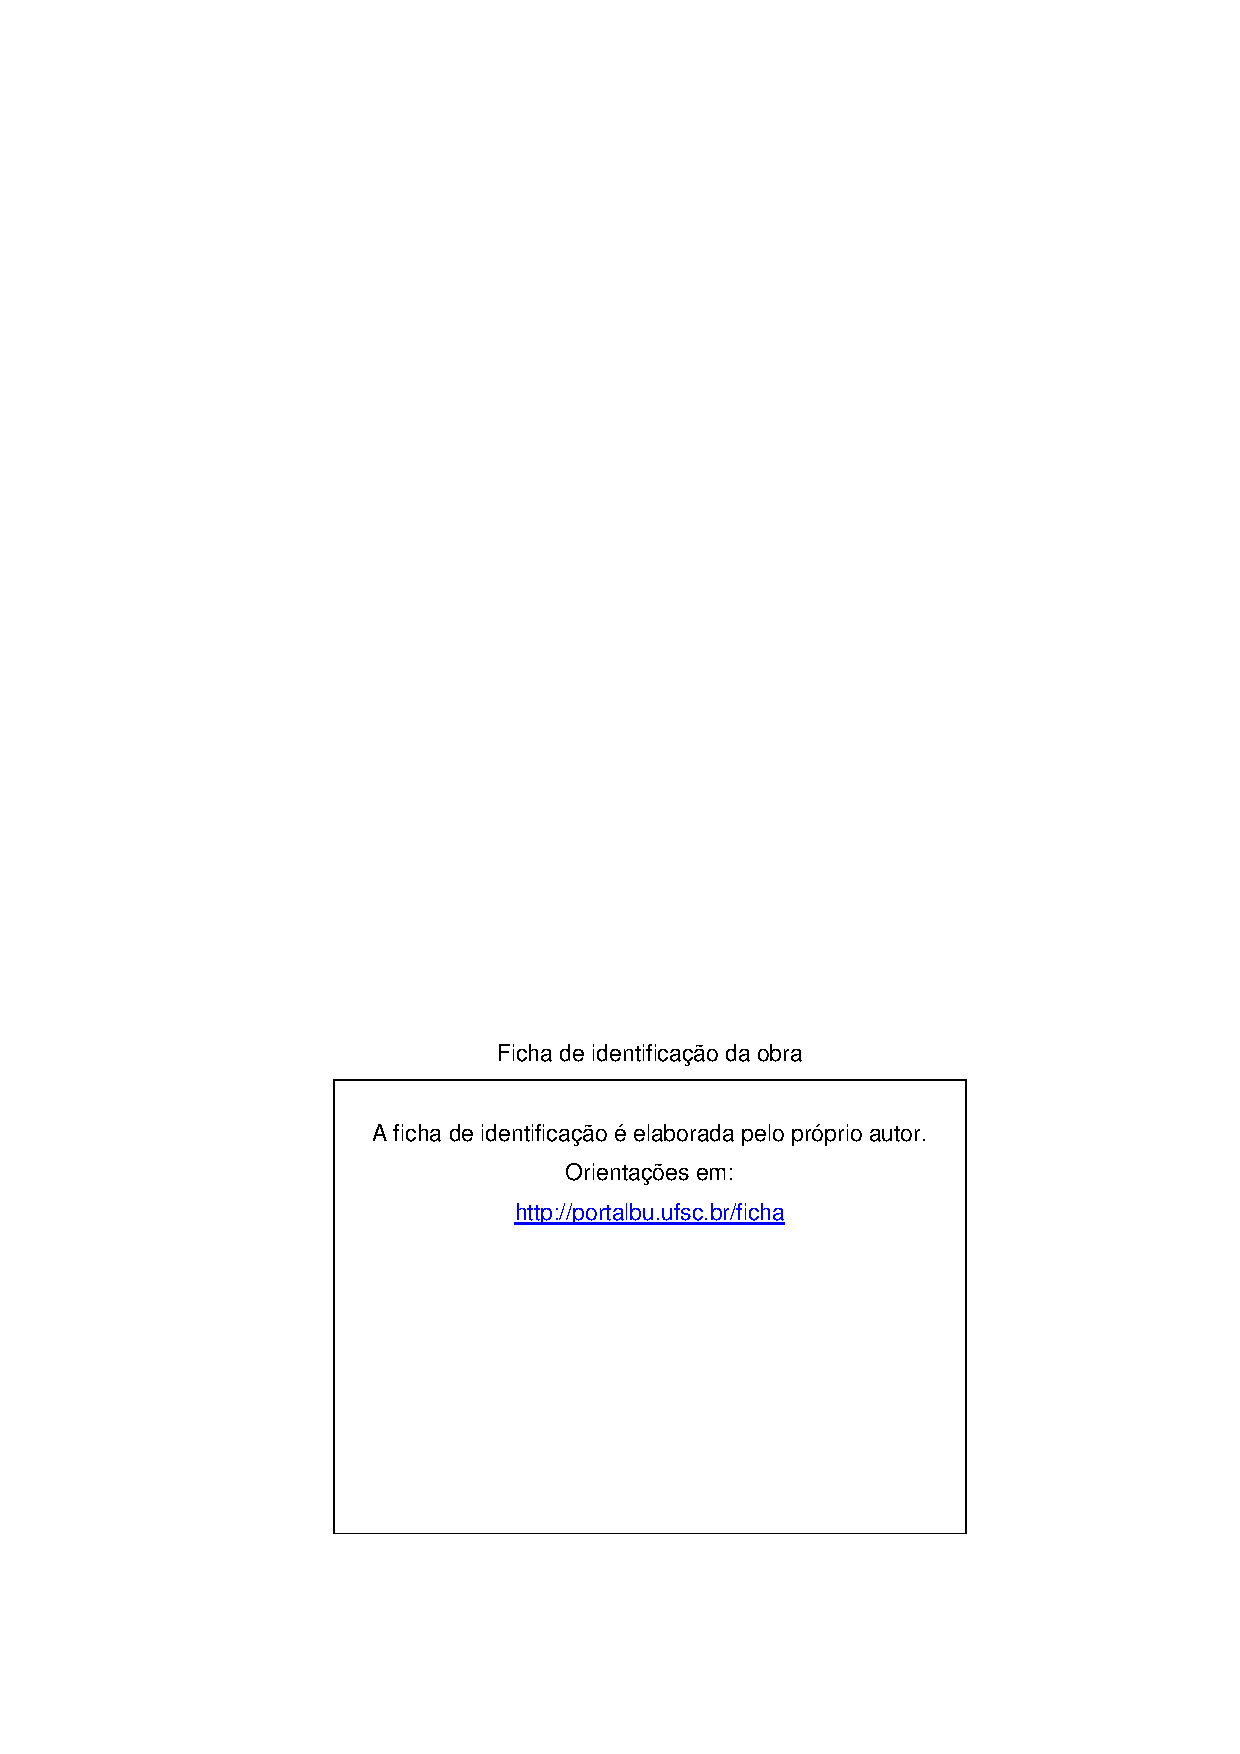
\includepdf{pre_textual/ficha_catalografica.pdf}
% \end{fichacatalografica}

% % Inserir folha de aprovação
% \begin{folhadeaprovacao}
% 	\OnehalfSpacing
% 	\centering
% 	\imprimirautor\\%
% 	\vspace{24pt}		
% 	\textbf{\imprimirtitulo}%
% 	\ifnotempty{\imprimirsubtitulo}{:~\imprimirsubtitulo}\\%
% 	%		\vspace*{31.5pt}%3\baselineskip
% 	\vspace*{\baselineskip}
% 	%\begin{minipage}{\textwidth}
% 	Este Trabalho de Conclusão de Curso foi julgao adequado para obtenção do Título de ``\imprimirformacao'' e aprovado em sua forma final pelo Curso de Graduação em Engenharia de Controle e Automação.\\
% 	\vspace{12pt}
% 	\imprimirlocal, \imprimirdia~de~\imprimirmes~de~\imprimirano.\\
	
% 	\vspace*{18pt}
% 	\textbf{Banca Examinadora:}\\
	
% 	\vspace*{24pt}
% 	\assinatura{\OnehalfSpacing \imprimirbancanomea}
% 	\vspace{6pt}
% 	\imprimirbancainsta\\
	
% 	\vspace*{24pt}
% 	\assinatura{\OnehalfSpacing \imprimirbancanomeb}
% 	\vspace{6pt}
% 	\imprimirbancainstb\\
	
% 	\vspace*{24pt}
% 	\assinatura{\OnehalfSpacing \imprimirbancanomec}
% 	\vspace{6pt}
% 	\imprimirbancainstc\\
	
% \end{folhadeaprovacao}

% Dedicatória
\ifnotempty{\imprimirdedicatoriatcc}{
\begin{dedicatoria}
	\vspace*{\fill}
	\noindent
	\begin{adjustwidth*}{}{7.5cm} 
		\textit{\imprimirdedicatoriatcc}
	\end{adjustwidth*}
\end{dedicatoria}
}

% Agradecimentos
\ifnotempty{\imprimiragradecimentostcc}{
\begin{agradecimentos}
	\imprimiragradecimentostcc
\end{agradecimentos}
}

% EPÍGRAFE
%\IFNOTEMPTY{\IMPRIMIREPIGRAFETCC}{
%\BEGIN{EPIGRAFE}
	%\VSPACE*{\FILL}
        %\NOINDENT
	%\BEGIN{ADJUSTWIDTH*}{}{7.5CM}
	       %\TEXTIT{\IMPRIMIREPIGRAFETCC}
        %\END{ADJUSTWIDTH*}
%\END{EPIGRAFE}
%}


% Resumo
\setlength{\absparsep}{18pt} % ajusta o espaçamento dos parágrafos do resumo
\begin{resumo}
	\SingleSpacing
	\imprimirresumotcc
	
	\textbf{Palavras-chave}: \imprimirpalavraschave
\end{resumo}

% Abstract
\begin{resumo}[Abstract]
	\SingleSpacing
	\imprimirabstracttcc
		
	\textbf{Keywords}: \imprimirkeywords
\end{resumo}

% Inserir publicações. Caso não deseje informa comentar todo esse bloco de código
% \begin{folhadeaprovacao}

% \cleardoublepage
% \begin{center}
%   {\textbf{PUBLICAÇÕES \textcolor{red}{Está página é opcional}}}
% \end{center}
% Esta dissertação é baseada no(s) artigo(s) científico(s) publicado(s) na(s) seguinte(s) revista(s):
% \vspace{1em}
% \begin{itemize}
%   \item SANTIAGO, Wagner Carvalho; KROETZ, Henrique Machado; SANTOS, Sérgio Hampshire de C.; STUCCHI, Fernando Rebouças; BECK, André Teófilo. Reliability-based calibration of main Brazilian structural design codes. \textbf{Latin American Journal of Solids and Structure}s, v. 17, e245, fev. 2020.
% \end{itemize}
% \cleardoublepage
	
% \end{folhadeaprovacao}

{%hidelinks
	\hypersetup{hidelinks}
	
	% inserir lista de figuras
	\pdfbookmark[0]{\listfigurename}{lof}
	\listoffigures*
	\cleardoublepage
	
	% inserir lista de quadros
	\ifnotempty{\verificaquadros}{
		\pdfbookmark[0]{\listofquadrosname}{loq}
		\listofquadros*
		\cleardoublepage
	}
	
	% inserir lista de tabelas
	\pdfbookmark[0]{\listtablename}{lot}
	\listoftables*
	\cleardoublepage
	
	% inserir lista de abreviaturas e siglas (devem ser declarados no preambulo)
	\ifnotempty{\verificasiglas}{
	\imprimirlistadesiglas
	}
	
	% inserir lista de símbolos (devem ser declarados no preambulo)
	\ifnotempty{\verificasimbolos}{
	\imprimirlistadesimbolos
	}

	% inserir o sumario
	\pdfbookmark[0]{\contentsname}{toc}
	\tableofcontents*
	\cleardoublepage
	
}%hidelinks

	% Elementos textuais
	\textual
	
	% 1 - Introdução
	% ----------------------------------------------------------
\chapter{Introdução}
% ----------------------------------------------------------

O concreto armado (CA) é um material fundamental na engenharia civil, com aplicação em uma vasta gama de construções, desde edifícios residenciais e comerciais até obras de infraestrutura de grande porte, como pontes e viadutos. Sua combinação da resistência à compressão do concreto com a ductilidade do aço confere aos elementos estruturais alta capacidade resistente e versatilidade construtiva. Entretanto, essas estruturas permanecem constantemente expostas a ambientes agressivos, tornando-as suscetíveis a processos de degradação que comprometem seu desempenho ao longo do tempo. Entre os mais relevantes, destaca-se a corrosão, que afeta diretamente a integridade das armaduras internas. 

A exposição contínua a esse mecanismo pode resultar em fissuração, perda de seção da armadura, destacamento do cobrimento e, consequentemente, redução da capacidade resistente de estruturas de concreto armado \cite{vu_structural_2000, pereira_junior_reliability_2023, soltani_state---art_2019, possan_co2_2016}. A perda de seção das armaduras longitudinais resulta na redução da rigidez e da resistência à flexão, enquanto a deterioração das armaduras transversais compromete a capacidade de cisalhamento e altera os modos de falha das vigas. Além disso, a degradação da aderência entre o concreto e o aço, induzida pela corrosão, prejudica a transferência de esforços internos, contribuindo para um desempenho estrutural globalmente inferior \cite{soltani_state---art_2019}.

A corrosão das armaduras em vigas de concreto armado pode ser classificada em dois tipos principais: a corrosão induzida por carbonatação e a induzida por cloretos. A carbonatação é um processo químico no qual o dióxido de carbono (CO\(_2\)) presente na atmosfera penetra nos poros do concreto e reage com o hidróxido de cálcio (Ca(OH)\(_2\)), formando carbonato de cálcio (CaCO\(_3\)) e reduzindo o pH da matriz cimentícia, conforme descrito por \textcite{helene_p_r_l_concreto_1993, ortega_assessment_2016}. Essa queda de pH compromete a camada passiva que protege as armaduras, dando início ao processo corrosivo \cite{possan_co2_2016}. Já a penetração de cloretos, mais comum em ambientes marinhos ou regiões onde se utilizam sais descongelantes, acelera a corrosão por meio de mecanismos de difusão, conforme descrito por \textcite{vu_structural_2000}, com base na Lei de Fick.

Nesse cenário, a corrosão impacta diretamente a vida útil remanescente (VUR) das estruturas, tornando a previsão desse parâmetro uma tarefa essencial para assegurar a segurança estrutural e planejar intervenções de manutenção de forma eficiente. A VUR tem como objetivo estimar o intervalo de tempo residual no qual uma estrutura ainda poderá desempenhar sua função com segurança. Essa estimativa parte do estado atual da estrutura e se estende até o momento em que ela perde os requisitos que definem sua durabilidade: a segurança e a funcionalidade. Segundo \textcite{bertolini_corrosion_2013} e \textcite{mehta_concrete_2014}, a durabilidade de uma estrutura está diretamente relacionada à capacidade do concreto em proteger as armaduras contra a corrosão por carbonatação e em manter suas propriedades mecânicas sob exposição a ambientes agressivos.

Na prática, a avaliação da VUR permite transformar dados de degradação, como profundidade de carbonatação, perda de seção das armaduras ou aumento da probabilidade de falha, em estimativas quantitativas do tempo restante até a necessidade de intervenção. \textcite{bertolini_corrosion_2013, okoh_overview_2014} destacam que modelos baseados em confiabilidade, que combinam a evolução da carbonatação com a perda de capacidade resistente e a redução do índice de confiabilidade estrutural, são ferramentas eficazes para essa estimativa. Além disso, estudos recentes \cite{silva_statistical_2016, zhang_prediction_2018} apontam que a integração entre monitoramento, simulação probabilística e técnicas de amostragem, como Monte Carlo, fornece uma base metodológica robusta para decisões de manutenção baseadas em risco. 

Nesse contexto, a previsão da vida útil remanescente constitui o principal objetivo deste trabalho, por meio do desenvolvimento de um modelo preditivo capaz de estimar o tempo em que o índice de confiabilidade atinge o limiar mínimo aceitável para estruturas de concreto armado. O modelo será capaz de considerar o tempo já decorrido de utilização da estrutura e, a partir disso, estimar o período de vida útil restante. As metodologias probabilísticas destacam-se nesse processo por oferecerem uma abordagem robusta para a avaliação de diferentes cenários, considerando as incertezas inerentes aos parâmetros materiais, geométricos e de carregamento. Conforme apontado por \textcite{pereira_junior_reliability_2023}, essa abordagem permite analisar o desempenho estrutural em distintos níveis de degradação, proporcionando resultados mais realistas e abrangentes.

Contudo, o simples emprego de regressores supervisionados sobre bases sintéticas apresenta uma limitação conceitual que merece destaque. Modelos de regressão convencionais fornecem uma predição \textit{pontual} do tempo de vida útil, ao passo que a decisão de manutenção sob incerteza requer a \textit{distribuição de probabilidade} desse tempo, da qual se extraem quantis inferiores e métricas de risco de cauda. Essa distinção é essencial: a incerteza reportada por um regressor descreve o erro do próprio modelo, e não a variabilidade intrínseca do processo de degradação. Para superar essa limitação, esta dissertação incorpora o arcabouço dos emuladores estocásticos, no qual a distribuição condicional completa da função de estado limite é aproximada por uma Distribuição Lambda Generalizada, cujos parâmetros são representados por Expansão em Caos Polinomial das variáveis de entrada e interpolados continuamente no tempo por um modelo de aprendizado de máquina \cite{ZhuSudret2020, ZhuSudret2021}. Uma vez treinado, o emulador fornece instantaneamente a densidade de probabilidade da margem de segurança em qualquer instante do horizonte de análise, da qual derivam a probabilidade de falha, a distribuição do tempo até a falha, a vida útil remanescente probabilística e as métricas de risco associadas.

O modelo desenvolvido como produto final desta pesquisa consistirá em uma ferramenta computacional, fundamentada em um referencial probabilístico, voltada a subsidiar decisões de manutenção e reforço de estruturas de concreto armado afetadas pela carbonatação, oferecendo suporte quantitativo à gestão da durabilidade estrutural.


\section{Objetivos}

\subsection{Objetivo Geral}

Desenvolver uma metodologia integrada, baseada em simulação de Monte Carlo, emulação estocástica e algoritmos de aprendizado de máquina, para avaliar a confiabilidade de estruturas de concreto armado submetidas à corrosão induzida por carbonatação e, a partir disso, determinar de forma probabilística sua vida útil remanescente (VUR), com o propósito de fornecer uma ferramenta prática, precisa e escalável para análise de risco e suporte à tomada de decisão em manutenção e gestão estrutural.

\subsection{Objetivos Específicos}

\begin{alineas}
    \item Representar numericamente os processos de degradação das propriedades mecânicas do concreto e das armaduras ao longo do tempo, considerando os efeitos da corrosão induzida por carbonatação.
    \item Gerar um banco de dados sintético por meio de simulações de Monte Carlo, incorporando a variabilidade de parâmetros geométricos, mecânicos e de carregamento.
    \item Aplicar algoritmos de aprendizado de máquina para modelar a evolução do índice de confiabilidade ($\beta$) e prever a vida útil remanescente (VUR) das estruturas em função de suas características e condições de exposição.
    \item Desenvolver um emulador estocástico dependente do tempo, capaz de aproximar a distribuição condicional completa da função de estado limite por meio da Distribuição Lambda Generalizada acoplada à Expansão em Caos Polinomial, com interpolação temporal contínua dos parâmetros da distribuição por aprendizado de máquina.
    \item Verificar o emulador proposto em problema de referência com solução de Monte Carlo direta, quantificando a aderência distribucional por testes estatísticos, comparação de quantis e ganho de eficiência computacional.
    \item Derivar da distribuição emulada as grandezas de interesse para a gestão de ativos: a probabilidade de falha dependente do tempo, a distribuição do tempo até a falha, a VUR probabilística e métricas de risco de cauda (VaR e CVaR).
    \item Incorporar métricas de incerteza, como intervalos de predição e largura de banda de confiança, para avaliar a robustez e a confiabilidade dos modelos desenvolvidos.
    \item Validar o desempenho dos modelos preditivos por meio de métricas estatísticas de erro, análises de sensibilidade e simulações independentes, garantindo sua aplicabilidade prática em diferentes cenários estruturais.
\end{alineas}


\section{Justificativa do Tema}

O concreto armado constitui o principal material estrutural utilizado na construção civil brasileira, sendo empregado em praticamente todos os tipos de obras, desde edifícios residenciais e comerciais até pontes, viadutos e barragens. Dessa forma, é possível afirmar que a grande maioria das construções urbanas no país utiliza algum tipo de estrutura de concreto armado, dada sua resistência mecânica, durabilidade e adaptabilidade a diferentes projetos. Essa predominância evidencia não apenas a importância estratégica dessas estruturas para a economia e a sociedade, mas também reforça a necessidade de estudos aprofundados sobre durabilidade, manutenção e vida útil, de modo a assegurar a segurança e a funcionalidade de um vasto parque construído ao longo das últimas décadas.

Por estarem constantemente expostas a ambientes agressivos, essas estruturas tornam-se suscetíveis a processos de degradação que comprometem seu desempenho ao longo do tempo. Dentre esses mecanismos, destaca-se a corrosão das armaduras induzida pela carbonatação, que reduz gradualmente a capacidade resistente das seções estruturais e, consequentemente, a vida útil da estrutura. Considerando a complexidade intrínseca desse fenômeno e a variabilidade dos parâmetros envolvidos, como propriedades dos materiais, condições ambientais e cargas aplicadas, torna-se essencial adotar ferramentas analíticas capazes de representar adequadamente tais incertezas. As abordagens determinísticas tradicionais, embora amplamente utilizadas, não conseguem capturar com precisão o comportamento probabilístico do sistema estrutural frente à degradação progressiva.

Nesse contexto, a aplicação de métodos probabilísticos, como a simulação de Monte Carlo, permite uma avaliação mais realista do tempo de vida útil remanescente das estruturas de concreto armado, incorporando a aleatoriedade dos parâmetros físicos e mecânicos. Além disso, a utilização de algoritmos de aprendizado de máquina possibilita a construção de modelos preditivos eficientes, capazes de generalizar padrões complexos a partir de grandes volumes de dados simulados.

A predição probabilística da vida útil remanescente oferece benefícios diretos significativos: possibilita o planejamento de manutenções baseadas em condições reais da estrutura, promove a alocação otimizada de recursos, aumenta a segurança ao identificar antecipadamente potenciais falhas e contribui para a sustentabilidade, ao permitir a extensão da vida útil das edificações sem comprometer sua integridade estrutural.

Dessa forma, a implementação de uma metodologia que integre simulação estocástica e aprendizado de máquina apresenta-se como uma solução robusta para a estimativa da vida útil de estruturas de concreto armado expostas à corrosão por carbonatação, fornecendo suporte quantitativo para decisões estratégicas de manutenção, reabilitação e gestão de ativos, com impactos diretos na durabilidade, segurança e eficiência do parque construído.

\section{Estrutura do Trabalho}

Além desta introdução, o texto está organizado em quatro capítulos.

O \autoref{cap:referencial} reúne o referencial teórico que sustenta a pesquisa, iniciando pelos fundamentos de confiabilidade estrutural e pelo método de amostragem de Monte Carlo com Hipercubo Latino. Em seguida, apresenta os modelos de resistência à flexão de vigas de concreto armado, com e sem a influência da corrosão das armaduras, e o modelo de avanço da frente de carbonatação. O capítulo trata ainda do conceito de vida útil remanescente e dos fundamentos de aprendizado de máquina, encerrando-se com a apresentação do arcabouço de emuladores estocásticos, que constitui o núcleo metodológico da segunda frente do trabalho.

O \autoref{met} descreve a metodologia adotada, organizada em duas frentes complementares: a construção do banco de dados sintético e o treinamento de modelos de regressão supervisionada, de um lado; e a construção do emulador estocástico dependente do tempo e a derivação, a partir da distribuição emulada, das grandezas de interesse para a gestão de ativos, de outro.

O \autoref{cap:resultados} apresenta os resultados obtidos até o presente estágio da pesquisa, incluindo a comparação entre algoritmos de regressão, a extração das estatísticas de vida útil remanescente, a verificação do emulador estocástico em problema de referência e o estado de desenvolvimento de sua aplicação ao problema da viga sob carbonatação. O capítulo encerra-se com o cronograma revisado de execução da pesquisa.

O \autoref{cap:consideracoes} consolida as considerações parciais que podem ser extraídas do estágio atual do trabalho, registra as limitações reconhecidas e delimita as etapas que restam para a conclusão da dissertação.

	
	% 2 - Referencial Teórico
	% ----------------------------------------------------------
\chapter{Referencial Teórico} \label{cap:referencial}
% ----------------------------------------------------------

\section{Confiabilidade Estrutural}

A confiabilidade pode ser compreendida como a capacidade de um sistema, equipamento, estrutura ou processo de desempenhar suas funções de maneira consistente e previsível, sem apresentar falhas, dentro de um período determinado e sob condições específicas. Em termos práticos, representa o nível de confiança de que um determinado elemento continuará operando conforme esperado, garantindo um desempenho estável ao longo do tempo e diante das variáveis do ambiente em que está inserido \cite{melchers_structural_2017}.

Desse modo, na engenharia estrutural, a confiabilidade é uma disciplina que busca avaliar a probabilidade de uma estrutura manter seu desempenho seguro ao longo de sua vida útil, mesmo considerando incertezas inerentes ao processo. Essas incertezas podem estar associadas a variabilidades nas cargas atuantes, resistência e degradação dos materiais, qualidade da execução e limitações dos modelos de engenharia empregados no dimensionamento e análise da estrutura \cite{melchers_structural_2017, du_structural_2023}.

Essas incertezas podem surgir de fatores como variabilidade nas propriedades dos materiais, condições ambientais, processos construtivos e intensidade de cargas aplicadas. A análise de confiabilidade variante no tempo é uma metodologia adequada para modelar o impacto dessas incertezas sobre o desempenho estrutural ao longo da vida útil de uma estrutura, quantificando os riscos de falha e determinando margens de segurança apropriadas para diferentes condições de exposição e uso \cite{melchers_structural_2017, du_structural_2023, pereira_junior_reliability_2023}.

No estudo da confiabilidade estrutural, a compreensão e quantificação das incertezas são essenciais, dentro das limitações inerentes a cada tipo. As incertezas podem ser classificadas em três categorias: aleatórias (ou intrínsecas), epistêmicas e erro humano. As incertezas epistêmicas decorrem da falta de conhecimento ou de informações insuficientes sobre um determinado fenômeno. À medida que novos dados se tornam disponíveis, esse tipo de incerteza pode ser reduzido ou até eliminado. Exemplos incluem simplificações na modelagem estrutural, aproximações na aplicação de cargas e definição das propriedades dos materiais \cite{du_structural_2023}.

As incertezas aleatórias, por outro lado, são inerentes aos processos físicos envolvidos e não podem ser completamente eliminadas, apenas reduzidas. Entre os principais exemplos, estão as variações naturais das propriedades dos materiais, as oscilações nas condições ambientais e os carregamentos que apresentam comportamento probabilístico. Além disso, o erro humano é um fator que pode influenciar todas as etapas da concepção, execução e manutenção das estruturas, contribuindo para a incerteza global do sistema. A correta identificação e quantificação dessas incertezas são fundamentais para a análise de confiabilidade estrutural, permitindo avaliar os riscos associados ao desempenho da estrutura ao longo de sua vida útil \cite{du_structural_2023}.

Entre os métodos de cálculo da confiabilidade pode-se citar: (\textit{a}) o Método de Primeira Ordem de Confiabilidade (FORM) que utiliza uma linearização da superfície de falha para obter estimativas rápidas e eficientes da probabilidade de falha (Soltani et al., 2021); (\textit{b}) Já o Método de Segunda Ordem de Confiabilidade (SORM) considera a curvatura da superfície de falha, proporcionando estimativas mais precisas; (\textit{c}) Os métodos de amostragem como a Simulação de Monte Carlo é amplamente é utilizada por sua flexibilidade em lidar com modelos complexos, gerando inúmeras amostras aleatórias para modelar o comportamento das variáveis e estimar a probabilidade de falha \cite{pereira_junior_reliability_2023}.

 Para estruturas sujeitas à corrosão, modelos probabilísticos são ferramentas eficazes para integrar variáveis como perda de massa das armaduras, concentração de cloretos e profundidade do cobrimento, fornecendo estimativas precisas das probabilidades de falha e orientando decisões sobre manutenção ou reforço (Vu e Stewart, 2000). A análise probabilística de uma estrutura tem como ponto de partida uma equação conhecida como “Equação de Estado Limite”. Essa equação, expressa por meio da função de estado limite $g(\mathbf{X})$, é uma formulação matemática que descreve o comportamento estrutural com base em critérios de segurança e desempenho estabelecidos para uma determinada condição de uso. De forma geral, essa função pode ser representada conforme a Equação \eqref{eq:g}.

\begin{equation}\label{eq:g}
g(\mathbf{X}) = g(X_1, X_2, X_3, \dots, X_n)
\end{equation} 

A análise da Equação \eqref{eq:g} permite concluir que a falha ocorre quando $g(\textbf{X})\leq0$. Em contraste, quando $g(\textbf{X}) > 0$, a estrutura é considerada segura, pois sua resistência é maior do que as solicitações que atuam sobre ela. Vale ressaltar que a falha nem sempre significa o colapso da estrutura; muitas vezes, ela está relacionada apenas ao não cumprimento de uma verificação específica, definida pela função de falha, onde os valores da variável de solicitação podem ter atingido ou ultrapassado os limites estabelecidos. Quando a Equação de Estado Limite é aplicada no contexto do Estado Limite Último (ELU), ela pode ser interpretada como a margem de segurança da estrutura, conforme expresso na Equação \eqref{eq:g_geral}, em que $\textbf{R}$ representa a resistência da estrutura e $\textbf{S}$ a solicitação atuante.

\begin{equation}\label{eq:g_geral}
g(\mathbf{R}, \mathbf{S}) = \textbf{R} - \textbf{S}
\end{equation} 

Com base nessa Equação de Estado Limite, é possível calcular tanto a probabilidade de falha quanto a de sobrevivência de um elemento estrutural. Conforme explicado por Beck (2019a), a probabilidade de falha de um sistema ou componente estrutural é determinada pela integração da função conjunta de densidade de probabilidade $f_x(\textbf{X})$ no domínio de falha, ou seja, quando $g(\textbf{X})\leq0$, como mostrado na Equação \eqref{eq:pf_geral}.

\begin{equation}\label{eq:pf_geral}
p_f = P[g(\mathbf{X})\leq 0] = \int_{g(\mathbf{X})\leq 0} f_x(\textbf{X}) dx
\end{equation}

% Neste trabalho será adotada a solução por meio de um método de amostragem de Monte Carlo. O modelo parte do pressuposto de gerar um sistema aleatório de partículas com base em uma determinada distribuição de probabilidade. Existem diversas variações do método de Monte Carlo. Neste trabalho, foi utilizado o Monte Carlo com Hipercubo Latino. A estimativa da probabilidade de falha utilizando o método de Monte Carlo é dada pela Equação \eqref{eq:p_f_sum}.

% \begin{equation}
% \label{eq:p_f_sum}
% \hat{p}_f = \frac{1}{n_s} \sum_{i=1}^{n_s} I_f
% \end{equation}

% \begin{equation}
% \label{eq:indicator}
% I_f = 
% \begin{cases}
% 1, & \text{se } g(\mathbf{X}) \leq 0 \\
% 0, & \text{caso contrário}
% \end{cases}
% \end{equation}

% Na Equação \eqref{eq:p_f_sum}, $n_s$ indica o número de amostras. No caso da Equação \eqref{eq:indicator}, o retorno 1 indica falha da função de Estado Limite, ou seja, indica que a estrutura não atendeu a determinado critério, e o retorno 0 indica que a estrutura está na região segura de avaliação da função de Estado Limite. 

% Para calcular o índice de confiabilidade ($\beta$), a Equação \eqref{eq:beta} utiliza a função de distribuição acumulada inversa (CDF) da distribuição normal padrão, denotada como $\Phi^{-1}$.

% \begin{equation}
% \label{eq:beta}
% \beta = -\Phi^{-1}(\hat{p}_f)
% \end{equation}


\section{Método de Amostragem de Monte Carlo com Hipercubo Latino}

Neste estudo, adota-se o método de amostragem de Monte Carlo, cuja origem remonta à década de 1940, quando Ulam e Von Neumann empregaram técnicas probabilísticas para simular fenômenos físicos complexos, especialmente no contexto de cálculos nucleares e aleatórios \cite{ulam_s_monte_1948}. 
Com o avanço da computação, tornou-se uma ferramenta essencial para estimar probabilidades integrando funções de densidades multivariadas, especialmente em contextos onde o cálculo exato é impraticável \cite{song_monte_2023}. 

O modelo parte do pressuposto de gerar um sistema aleatório de partículas com base em uma determinada distribuição de probabilidade. 
Em confiabilidade estrutural, o estimador de falha usual emprega uma função indicadora $I_f$, conforme apresentado na Equação~\eqref{eq:p_f_sum}, onde a probabilidade de falha é estimada por:

\begin{equation}
\label{eq:p_f_sum}
\hat{p}_f = \frac{1}{n_s} \sum_{i=1}^{n_s} I_f
\end{equation}

\begin{equation}
\label{eq:indicator}
I_f =
\begin{cases}
1, & \text{se } g(\mathbf{X}) \leq 0 \\
0, & \text{caso contrário}
\end{cases}
\end{equation}

Na Equação~\eqref{eq:p_f_sum}, $n_s$ indica o número de amostras. 
No caso da Equação~\eqref{eq:indicator}, o retorno $1$ indica falha da função de Estado-Limite, ou seja, que a estrutura não atendeu a determinado critério, e o retorno $0$ indica que a estrutura está na região segura da função de Estado-Limite.

Para calcular o índice de confiabilidade ($\beta$), a Equação~\eqref{eq:beta} utiliza a função de distribuição acumulada inversa (CDF) da distribuição normal padrão, denotada como $\Phi^{-1}$.

\begin{equation}
\label{eq:beta}
\beta = -\Phi^{-1}(\hat{p}_f)
\end{equation}

Existem diversas variações do método de Monte Carlo. Neste trabalho, adotou-se a técnica de Monte Carlo com Hipercubo Latino (\textit{Latin Hypercube Sampling} — LHS), originalmente proposta por \textcite{mckay_comparison_1979} como uma forma de amostragem estratificada voltada à redução da variância das estimativas, quando comparada à amostragem puramente aleatória.

No campo da análise de confiabilidade estrutural, o LHS tem sido amplamente empregado por sua capacidade de aprimorar a eficiência e a representatividade do espaço amostral, assegurando uma distribuição mais uniforme em cada dimensão marginal. Essa característica permite estimar probabilidades de falha com menor número de amostras redundantes, mantendo a precisão dos resultados \cite{helton_latin_2003}.

A utilização do LHS neste estudo tem como objetivo reduzir a variabilidade das estimativas de probabilidade de falha, especialmente em problemas de alta dimensionalidade, proporcionando uma amostragem de boa qualidade sem a necessidade de um número excessivo de simulações \cite{melchers_structural_2017}.

De forma análoga à amostragem estratificada, o método do Hipercubo Latino divide o domínio de cada variável aleatória em intervalos equiprováveis \cite{helton_latin_2003, olsson_latin_2003, helton_signal_2005}. Cada intervalo é amostrado exatamente uma vez, garantindo uma distribuição espaçada e uniforme dos pontos no espaço amostral. Essa propriedade assegura uma cobertura mais homogênea do domínio das variáveis. Um exemplo ilustrativo para o caso bidimensional é apresentado na Figura \ref{fig:lhs}.

\begin{figure}[H]
    \centering
    \caption{Exemplo de correlação entre variáveis no Hipercubo Latino.}
    \label{fig:lhs}
    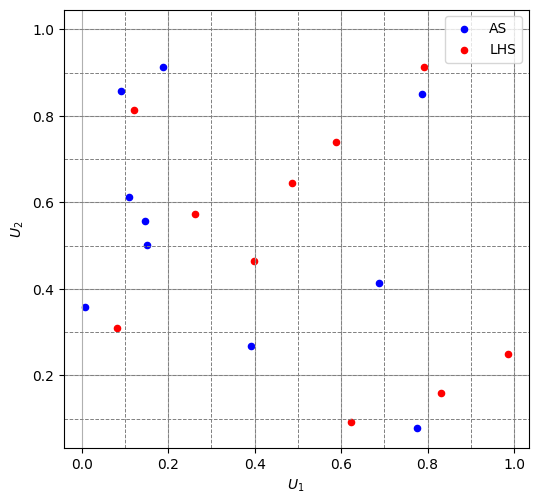
\includegraphics[width=0.7\linewidth]{lhs.png}
    \fonte{Autor (2025).}
\end{figure}

Considerando $n$ o número de variáveis aleatórias e $n_s$ o total de amostras geradas, define-se a matriz $P$ de dimensões $(n_s \times n)$, cujas colunas
$P_j = \pi_j(1, 2, \ldots, n_s)$ representam permutações aleatórias da sequência $(1, \ldots, n_s)$, de modo a evitar correlações artificiais entre as variáveis amostradas.
Em seguida, é construída uma matriz $R \in (0,1)_{n_s \times n}$, cujos elementos são mutuamente independentes e seguem uma distribuição uniforme $U(0,1)$ \cite{olsson_latin_2003}.  
Com base nessas duas matrizes, obtém-se a matriz $S$ (Equação \eqref{eq:S_matrix}):

\begin{equation}
S = [s_{ij}]_{n_s \times n} 
= \frac{1}{n_s} (P - R).
\label{eq:S_matrix}
\end{equation}

As amostras normalizadas são então determinadas a partir de $S$ conforme a Equação \eqref{eq:x_samples}:

\begin{equation}
X_j = \{ x_i \}_{i=1,\ldots,n_s} 
= \left\{ F^{-1}_{X_j}(s_{ij}) \right\}_{i=1,\ldots,n_s},
\label{eq:x_samples}
\end{equation}

em que $F^{-1}_{X_j}$ corresponde à função inversa da distribuição acumulada da variável $X_j$.

Para casos em que o número de variáveis $n$ é elevado, a construção explícita das matrizes $P$, $R$ e $S$ pode demandar grande capacidade de armazenamento. Assim, o processo pode ser otimizado sem a necessidade de armazenar as matrizes completas, conforme descrito a seguir:

\vspace{1em}

\textbf{Procedimento para geração dos elementos $x_{ij}$ sem formar as matrizes completas:}  
\begin{enumerate}
    \item Para cada variável $j = 1, \dots, n$, faça:
    \item[] \quad Obtenha o vetor $P_j$, correspondente à $j$-ésima coluna de $P$, composta por uma permutação da sequência $(1, \dots, n_s)$.
    \item Para cada amostra $i = 1, \dots, n_s$, execute:
    \item[] \quad Gere um número aleatório $r \sim U(0,1)$.
    \item[] \quad Calcule $s_{ij} \gets \dfrac{p - r}{n_s}$.
    \item[] \quad Determine $x_{ij} \gets F_{X_j}^{-1}(s_{ij})$.
    \item[] \textbf{Fim do loop sobre $i$}
    \item[] \textbf{Fim do loop sobre $j$}
\end{enumerate}


\section{Resistência de Vigas de Concreto Armado sem Influência da Corrosão das Armaduras}

O cálculo da resistência de uma viga de concreto armado sem corrosão considera a integridade total dos materiais, levando em conta a resistência característica do concreto ($f_{ck}$), a área da seção transversal e a armadura longitudinal projetada. Nessa condição, o momento resistente ($M_{Rd,lim}$) é determinado conforme a Equação \eqref{eq:mrd_lim}, caracterizando assim o Momento resistente no estado limite último da capacidade de resistência da seção a flexão no Estádio III devido às cargas normais, conforme definido pela NBR 6118 \cite{associacao_brasileira_de_normas_tecnicas_nbr_2023}:

\begin{equation}\label{eq:mrd_lim}
M_{Rd,lim} = r_{cc} \cdot \left( d - 0.5 \cdot \lambda_c \cdot x \right)
\end{equation}

\begin{equation}\label{eq:r_cc}
r_{cc} = \sigma_{cd} \cdot \left( \lambda_c \cdot x \cdot b_w \right)
\end{equation}

\begin{equation}\label{eq:sigma_cd}
\sigma_{cd} = \alpha_c \cdot \eta_c \cdot (f_{ck}/\gamma_c)
\end{equation}

O momento resistente da seção ($M_{Rd,lim}$) representa a capacidade de resistência da viga frente aos esforços fletores. O termo ($r_{cc}$) corresponde à tensão de cálculo do concreto na compressão, determinada a partir da resistência característica do concreto e das condições geométricas da seção. A profundidade útil da seção é indicada por ($d$), enquanto ($x$) representa a altura da zona comprimida do concreto e ($\lambda_c$) é o coeficiente que define a distribuição de tensões na seção, influenciando o cálculo do momento resistente. A tensão de cálculo do concreto ($\sigma_{cd}$) é obtida considerando os fatores de redução normativos ($\alpha_c$ e $\eta_c$) e a resistência de cálculo do concreto ($f_{cd}$), os quais ajustam a capacidade do material segundo critérios de segurança. Por fim, ($b_w$) representa a largura efetiva da seção transversal, que contribui diretamente para a determinação da tensão de compressão e, consequentemente, para o momento resistente da viga.

A resistência de cálculo do concreto é dada pela Equação \eqref{eq:fcd}:

\begin{equation}\label{eq:fcd}
f_{cd} = \frac{f_{ck}}{\gamma_c}
\end{equation}

onde $\gamma_c$ é o coeficiente parcial de segurança do concreto. Os parâmetros $\alpha_c$, $\eta_c$ e $\lambda_c$ variam em função da resistência característica à compressão do concreto ($f_{ck}$), conforme as Equações \eqref{eq:lambda_c}, \eqref{eq:alpha_c} e \eqref{eq:eta_c}, recomendadas pela NBR 6118 \cite{associacao_brasileira_de_normas_tecnicas_nbr_2023}:

\begin{equation}\label{eq:lambda_c}
\lambda_c =
\begin{cases}
0.80, & f_{ck} \leq 50~\text{MPa} \\
0.80 - \displaystyle\frac{(f_{ck} - 50)}{400}, & f_{ck} > 50~\text{MPa}
\end{cases}
\end{equation}

\vspace{6pt}

\begin{equation}\label{eq:alpha_c}
\alpha_c =
\begin{cases}
0.85, & f_{ck} \leq 50~\text{MPa} \\
(1.00 - \displaystyle\frac{(f_{ck} - 50)}{200}) \cdot 0.85, & f_{ck} > 50~\text{MPa}
\end{cases}
\end{equation}

\vspace{6pt}

\begin{equation}\label{eq:eta_c}
\eta_c =
\begin{cases}
1.00, & f_{ck} \leq 50~\text{MPa} \\
\left( \displaystyle\frac{40}{f_{ck}} \right)^{1/3}, & f_{ck} > 50~\text{MPa}
\end{cases}
\end{equation}

\vspace{6pt}

Na prática, a relação $d/h$ é um parâmetro empírico adotado em função da altura da viga, do cobrimento e do diâmetro das barras de aço, variando tipicamente entre 0{,}85 e 0{,}95. Por fim, o coeficiente de segurança do aço ($\gamma_s$) ajusta a resistência característica à tração do aço ($f_{yk}$), resultando na tensão de cálculo de escoamento ($f_{yd}$), expressa pela Equação \eqref{eq:fyd}:

\begin{equation}\label{eq:fyd}
f_{yd} = \frac{f_{yk}}{\gamma_s}
\end{equation}

Para concluir o cálculo do momento resistente limite ($M_{Rd,lim}$), é necessário determinar a profundidade da linha neutra ($x$). Esta profundidade é obtida a partir do equilíbrio das forças normais entre a armadura tracionada e o concreto comprimido, resolvendo-se a função $f_\alpha(\beta) = 0$, que relaciona os esforços na seção transversal. Como a equação que define $x$ não admite solução analítica direta, recorre-se a métodos numéricos iterativos. No presente trabalho, utilizou-se o método da bisseção (\textit{bisection method}) para localizar a raiz de $f_\alpha(\beta)$ dentro de um intervalo pré-estabelecido. O procedimento iterativo pode ser descrito da seguinte forma:

\begin{enumerate}
    \item Definir um intervalo inicial $[\beta_{\min}, \beta_{\max}]$ no qual a raiz esteja contida.
    \item Calcular o ponto médio do intervalo: $\beta_m = (\beta_{\min} + \beta_{\max})/2$.
    \item Avaliar a função $f_\alpha(\beta_m)$. Caso $f_\alpha(\beta_m)$ seja próximo de zero dentro da tolerância predefinida, a solução foi encontrada.
    \item Caso contrário, atualizar o intervalo mantendo a raiz contida e repetir o processo até a convergência.
\end{enumerate}

A Figura \ref{fig:fluxograma}, apresentada a seguir, ilustra o fluxograma do processo iterativo.

\begin{figure}[H]
    \centering
    \caption{Fluxograma do processo iterativo de determinação da linha neutra ($x$) pelo método de bisseção.}
    \label{fig:fluxograma}
    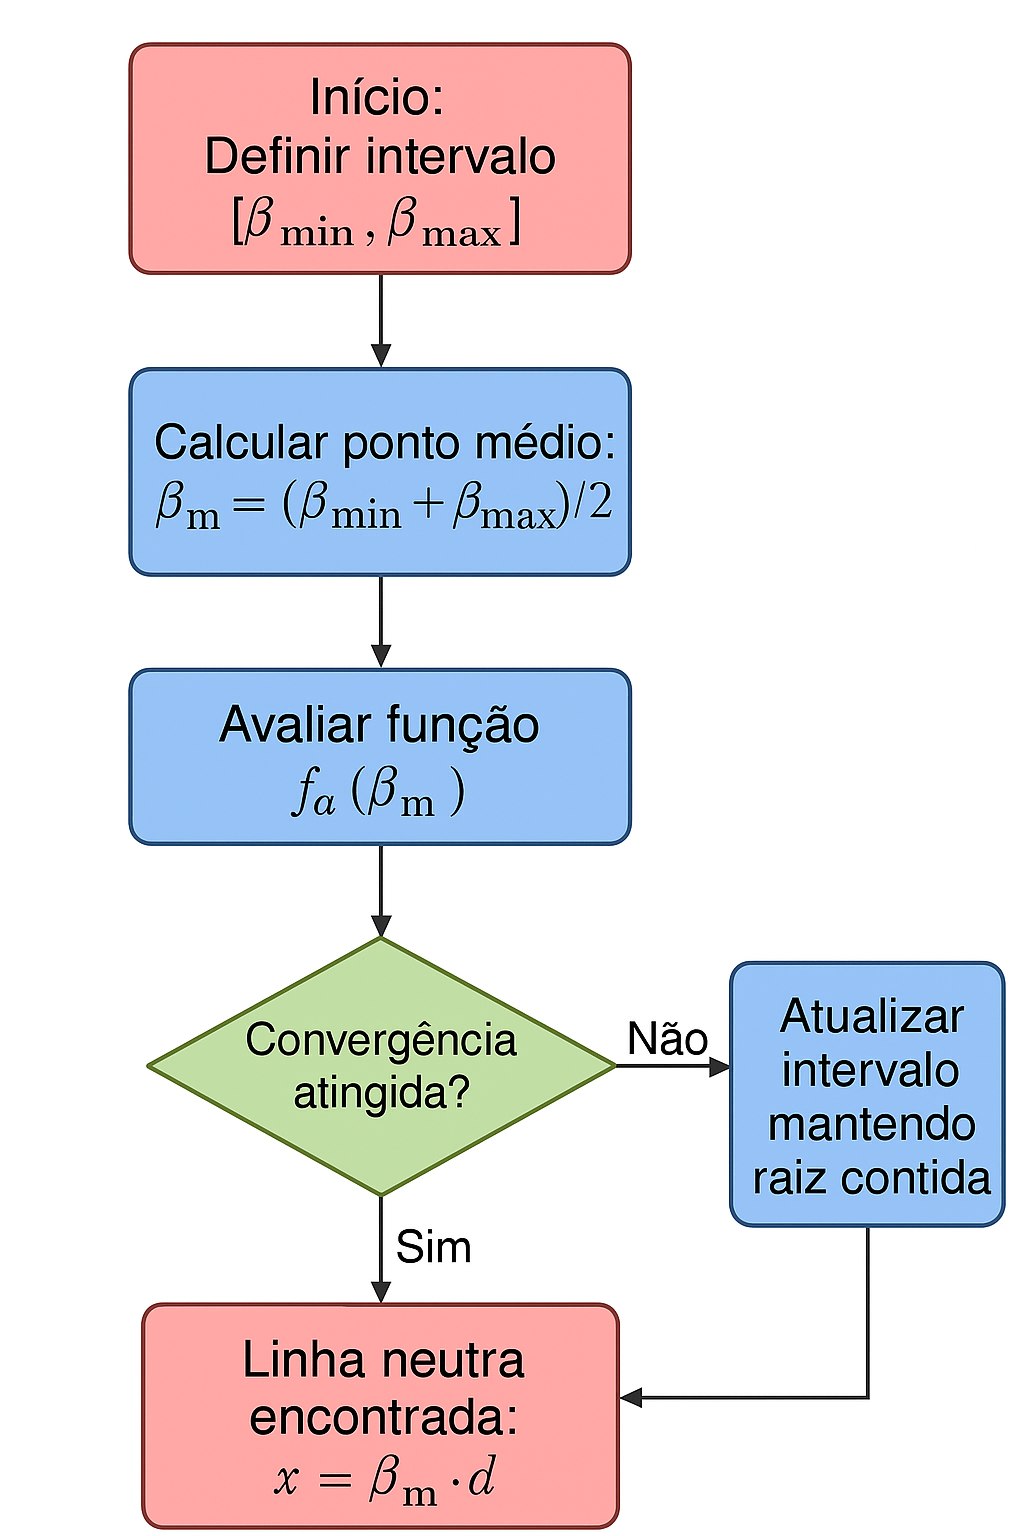
\includegraphics[width=0.45\linewidth]{fluxograma.png}
    \fonte{Autor (2025).}
\end{figure}

% \begin{algorithm}[H]
%   \caption{Determinação iterativa da linha neutra via método da bisseção}
%   \label{alg:determinacaoLinhaNeutra}
%   \begin{algorithmic}[H]
%     \Require intervalo inicial $[\beta_{\min}, \beta_{\max}]$, tolerância $\varepsilon$
%     \Ensure profundidade da linha neutra $x = \beta \cdot d$
%     \State defina $\beta_{\min}, \beta_{\max}$
%     \While{$\beta_{\max} - \beta_{\min} > \varepsilon$}
%       \State $\beta_m \gets (\beta_{\min} + \beta_{\max}) / 2$
%       \State $f_m \gets f_\alpha(\beta_m)$
%       \If{$|f_m| \le \varepsilon$}
%         \State \textbf{break}
%       \ElsIf{$f_\alpha(\beta_{\min}) \cdot f_m < 0$}
%         \State $\beta_{\max} \gets \beta_m$
%       \Else
%         \State $\beta_{\min} \gets \beta_m$
%       \EndIf
%     \EndWhile
%     \State $\beta \gets \beta_m$
%     \State $x \gets \beta \cdot d$
%     \State \textbf{return} $x$
%   \end{algorithmic}
% \end{algorithm}

A profundidade da linha neutra encontrada, $x = \beta \cdot d$, é então utilizada para determinar o momento resistente da seção de concreto armado, conforme descrito nas Equações \eqref{eq:mrd_lim}, \eqref{eq:r_cc} e \eqref{eq:sigma_cd}. Esse esquema garante que o cálculo do momento resistente considere corretamente o equilíbrio interno de forças e as propriedades não lineares do concreto e do aço.


\section{Resistência de Vigas de Concreto Armado Sujeitas a Corrosão por Carbonatação}

% \section{Momento resistente em vigas sujeita corrosão por carbonatação}

\subsection{Corrosão por Carbonatação}

Nas estruturas de concreto armado, o concreto desempenha um papel protetor fundamental para o aço, atuando em dois níveis distintos. Primeiramente, ele oferece uma proteção física, funcionando como uma barreira que impede o contato direto do aço com o ambiente externo. Em segundo lugar, proporciona uma proteção química, devido à presença de uma solução alcalina nos poros do concreto, que promove a formação de uma camada passivadora ao redor do aço. Essa camada é responsável por reduzir drasticamente as taxas de corrosão, uma vez que possui alta resistência elétrica e dificulta o acesso de umidade, oxigênio e substâncias agressivas à superfície do aço \cite{PaziniMeira2012}

Durante a vida útil de uma estrutura de concreto armado, dois períodos de corrosão podem ser distinguidos. O período de iniciação é caracterizado pelo estágio em que o reforço é protegido por uma fina camada de óxido, o que garante uma taxa de corrosão insignificante e a ausência de efeitos de deterioração. A segunda fase, o período de propagação, começa quando a cobertura de concreto é contaminada e a camada de óxido passivo é destruída, resultando em um aumento da taxa de corrosão e na deterioração da condição da estrutura \cite{cavaco_reliabilitybased_2017}.

A degradação de estruturas de concreto armado pela corrosão das armaduras representa um dos maiores desafios à durabilidade na engenharia civil, sendo a corrosão localizada por cloretos e a corrosão generalizada por carbonatação os dois processos mais prevalentes e estruturalmente significativos \cite{helene_p_r_l_concreto_1993}.  

A corrosão por cloretos caracteriza-se pelo ataque localizado (pites). Os íons cloreto difundem-se através do concreto até a armadura, adsorvem-se seletivamente na película passivante que cobre o aço e a rompem em pequenos pontos, criando microcélulas galvânicas. Conforme \textcite{mehta_concrete_2014}, esta configuração eletroquímica concentra a dissolução do metal em pequenas áreas, resultando em cavidades profundas que comprometem criticamente a capacidade estrutural, mesmo com perda mínima de massa global.

Em contraste, a corrosão por carbonatação opera de modo mais difuso, promovendo corrosão uniformemente distribuída ao longo da armadura quando a frente de carbonatação atinge o recobrimento. O dióxido de carbono atmosférico penetra nos poros do concreto, dissolve-se na água capilar dos poros, reagindo principalmente com hidróxido de cálcio (Ca(OH)\(_2\)) da pasta de cimento, segundo a reação química fundamental ilustrada pela Equação \eqref{eq:carbonatacao}:

\begin{equation}\label{eq:carbonatacao}
\mathrm{Ca(OH)_2 + CO_2 \rightarrow CaCO_3 + H_2O}
\end{equation}

Conforme essa reação ocorre, há consumo dos hidróxidos alcalinos que mantêm o concreto fortemente básico \cite{villain_measurement_2007}. A Figura \ref{fig:corrosão} ilustra de forma comparativa os diferentes mecanismos de atuação dos dois tipos de corrosão anteriormente descritos.

\begin{figure}[H]
    \centering
    \caption{Tipos de corrosão.}
    \label{fig:corrosão}
    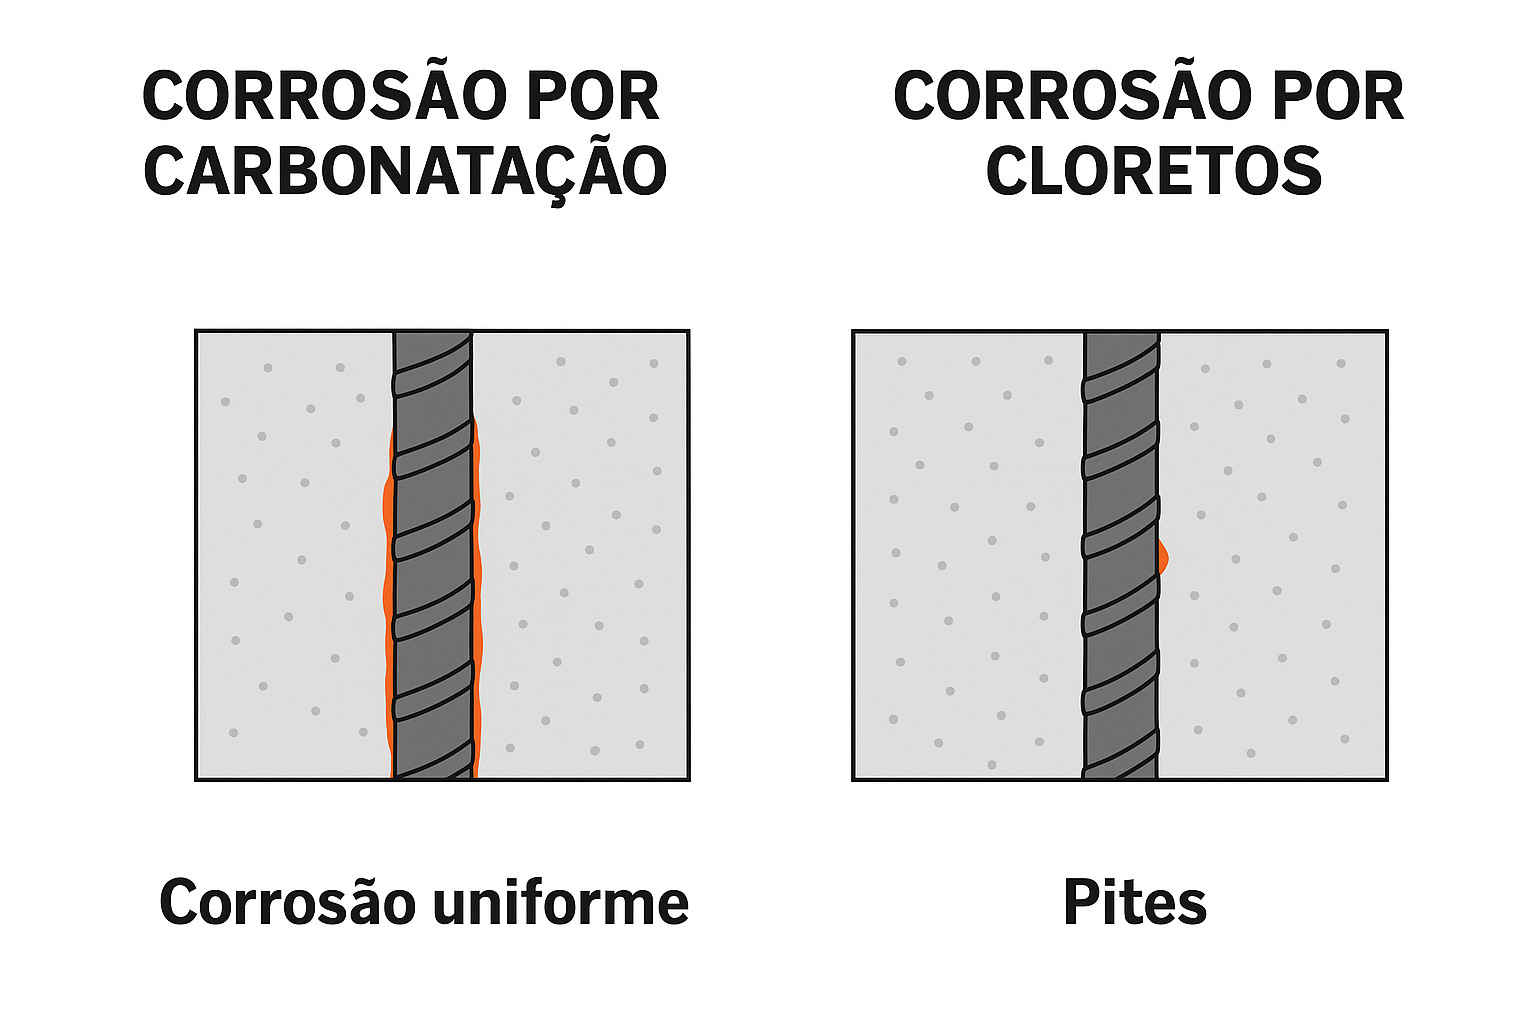
\includegraphics[width=0.6\linewidth]{corrosao.png}
    \fonte{Autor (2025).}
\end{figure}

Originalmente, o concreto apresenta pH interno bem elevado, tipicamente entre 12,5 e 13,5; à medida que a carbonatação avança, esse pH diminui significativamente, podendo atingir valores próximos de 8 a 9 antes de atingir a profundidade da armadura, momento em que o aço deixa de estar em regime passivo \cite{helene_p_r_l_concreto_1993}. A despassivação da armadura ocorre quando o filme protetor de óxidos/hidróxidos de ferro deixa de ser termodinamicamente estável neste ambiente de menor alcalinidade; exposto ao oxigênio e à água, o aço passa a corroer de modo ativo, de preferência de maneira mais uniforme ao longo da superfície que está atingida pela frente de carbonatação \cite{neville_properties_2011}.

Um aspecto crítico desse processo, bem documentado por \textcite{tuutti_corrosion_1982}, é que os produtos de corrosão (óxidos e hidróxidos de ferro) apresentam volume significativamente maior que o metal original, gerando forças de expansão internas no concreto circundante. Essa expansão causa tensões de tração no recobrimento que levam a fissuração (fendilhamento) e eventual destacamento da capa de concreto, o que por sua vez permite penetração adicional de agentes agressivos, acelerando o ciclo de degradação.

Nas décadas mais recentes, estudos têm quantificado com maior precisão as taxas de corrosão associadas à carbonatação, bem como os fatores que controlam essa taxa. \textcite{stefanoni_corrosion_2018} revisam diversos dados e concluem que, na fase de propagação em concreto carbonatado, além da extensão da carbonatação, são determinantes fatores como o grau de saturação dos poros, a área efetiva de aço em contato com poros cheios de água, a porosidade, a relação água/cimento, bem como a natureza dos cimentos usados.

Portanto, tanto a literatura clássica como os estudos modernos convergem para o entendimento de que:

\begin{itemize}
  \item A corrosão por cloretos gera danos severos localizados, muitas vezes com perdas de seção muito concentradas, mas inicia-se mesmo em condições em que o concreto mantém pH elevado (não requer carbonatação prévia).
  \item A carbonatação, por sua vez, é um processo mais lento, exigindo difusão de CO\(_2\), reação química com os hidróxidos alcalinos, redução do pH interno, despassivação do aço, e subsequente corrosão ativa, usualmente mais uniforme.
  \item O dano estrutural não decorre apenas da perda de seção, mas também dos efeitos físicos da expansão dos óxidos de ferro (fissuração/destacamento), que diminuem a proteção do recobrimento e aceleram os mecanismos de degradação.
  \item Fatores materiais (tipo de cimento, adições, porosidade, relação água/cimento, recobrimento) e ambientais (umidade relativa, temperatura, concentração de CO\(_2\), disponibilidade de oxigênio) controlam fortemente tanto a velocidade de carbonatação quanto a taxa de corrosão após despassivação.
\end{itemize}

A perda de área de seção transversal das armaduras reduz a capacidade de resistência às forças aplicadas, enquanto o aumento de volume dos produtos de corrosão gera tensões internas que resultam em fissuração do concreto e destacamento do cobrimento \cite{soltani_state---art_2019}. Além disso, a interface entre o aço e o concreto é comprometida, prejudicando a transferência de tensão entre os materiais \cite{vu_structural_2000, soltani_state---art_2019}.

Para mitigar os efeitos da corrosão, algumas medidas preventivas podem ser adotadas, como o aumento do cobrimento de concreto, o uso de inibidores de corrosão e o monitoramento contínuo com sensores para detectar precocemente a penetração de cloretos ou a carbonatação. Reparações localizadas e aplicação de revestimentos protetores também são cruciais para a manutenção da integridade estrutural.

% \begin{table}[H]
% \centering
% \footnotesize
% \caption{Comparação entre modelos matemáticos de previsão.}
% \label{tab:modelos_carbonatacao}
% \begin{tabular}{p{0.61\textwidth} p{0.36\textwidth}}
% \toprule
% \textbf{Modelo} & \makecell{\textbf{Escopo de Aplicação} \\ \textbf{e Confiabilidade}} \\
% \midrule

% \textbf{\textcite{zhang_prediction_2018}:} & 
% \multirow{9}{6cm}[0pt]{%
% \begin{enumerate}[leftmargin=*]
% \item O modelo é mais adequado para concretos com agregados reciclados.
% \item Os valores de $f_c$, $k_c$ e $T$ adotados são teóricos e podem divergir dos reais.
% \end{enumerate}} \\[2mm]
% $x = m \cdot k_A \cdot \sqrt{T} \cdot k_e \cdot \sqrt{\frac{k_c \cdot W}{f_c}} \cdot k_{CO_2} \cdot \sqrt{t}$ \\[1mm]
% $k_A$: absorção de água do agregado; \\
% $T$: temperatura; \\
% $k_e = RH^{1.5}(1 - RH)$, sendo $RH$ a umidade relativa; \\
% $k_c$: parâmetro de transferência de execução; \\
% $f_c$: resistência à compressão aos 28 dias (MPa); \\
% $W$: teor de água; \\
% $k_{CO_2}$: concentração de $CO_2$; \\
% $m$: parâmetro constante. \\[1mm]
% \textit{Parâmetros a serem medidos:} $RH$, $W$, $C$, $k_{CO_2}$. \\[2mm]
% \midrule

% \textbf{\textcite{silva_statistical_2016}:} &
% \multirow{6}{6cm}[0pt]{%
% \begin{enumerate}[leftmargin=*]
% \item Adequado para concretos com agregados reciclados.
% \item Considera principalmente o efeito do $EWA$ na carbonatação.
% \end{enumerate}} \\[2mm]
% $x = K_C \sqrt{t} = (72{,}470 - 0{,}772f_c - 0{,}117C_0 + 4{,}617c + 1{,}594EWA)\sqrt{t}$ \\
% $C_0$: teor de clínquer (kg/m³); \\
% $c$: teor de $CO_2$ no ambiente; \\
% $EWA$: absorção equivalente de água dos agregados reciclados (\%). \\[1mm]
% \textit{Parâmetros a serem medidos:} $C_0$, $c$, $EWA$. \\[2mm]
% \midrule

% \textbf{\textcite{wang_review_2024}:} &
% \multirow{5}{6cm}[0pt]{%
% \begin{enumerate}[leftmargin=*]
% \item O parâmetro $D_C$ é difícil de determinar na prática.
% \item O modelo considera principalmente o efeito do $CO_2$ na carbonatação.
% \end{enumerate}} \\[2mm]
% $x = \sqrt{\frac{2D_C \cdot c_c}{m_c}} \cdot \sqrt{t}$ \\[1mm]
% $D_C$: coeficiente efetivo de difusão de $CO_2$ no concreto; \\
% $c_C$: concentração de $CO_2$ no ambiente; \\
% $m_c$: absorção de $CO_2$ por unidade de concreto. \\[1mm]
% \textit{Parâmetros a serem medidos:} $C_c$, $m_c$. \\[2mm]
% \midrule

% \textbf{\textcite{papadakis_effect_2000}:} &
% \multirow{5}{6cm}[0pt]{%
% \begin{enumerate}[leftmargin=*]
% \item Aplicável apenas a concretos com cimento Portland comum.
% \item O modelo requer muitos parâmetros, dificultando sua aplicação prática.
% \end{enumerate}} \\[2mm]
% $x = \sqrt{\frac{C_{Ca(OH)_2}}{C_{CSH_1} + C_{CSH_2} + C_{C2S} + C_{C3S} + C_{C4C5}}} \cdot \sqrt{t}$ \\[1mm]
% $C_{Ca(OH)_2}$, $C_{CSH}$, $C_{C2S}$ e $C_{C3S}$: concentrações iniciais de hidróxidos e silicatos. \\[1mm]
% \textit{Parâmetros a serem medidos:} $C_{Ca}$, $C_{Ca(OH)_2}$, $C_{CSH}$, $C_{C3S}$, $C_{C2S}$. \\[2mm]
% \midrule

% \textbf{\textcite{wang_review_2024}:} &
% \multirow{5}{6cm}[0pt]{%
% \begin{enumerate}[leftmargin=*]
% \item Modelo altamente dependente da precisão do fator $w/c$.
% \item Considera principalmente o efeito do tipo de cimento, agregados e aditivos.
% \end{enumerate}} \\[2mm]
% $x = f_k \cdot k_g \cdot k_s \sqrt{\frac{w/c - 0{,}25}{0{,}3(1{,}5 + 3a/(w/c))}} \cdot \sqrt{t}$, para $w/c > 0{,}6$ \\[1mm]
% $k$: coeficiente de influência do tipo de cimento; \\
% $k_g$: coeficiente de influência dos agregados; \\
% $k_s$: coeficiente de influência dos aditivos; \\
% $w/c$: relação água/cimento. \\[1mm]
% \textit{Parâmetro a ser medido:} $w/c$. \\[2mm]
% \midrule

% \textbf{\textcite{article}:} &
% \multirow{4}{6cm}[0pt]{%
% \begin{enumerate}[leftmargin=*]
% \item O modelo é muito sensível à precisão da relação $w/c$.
% \item Os resultados de previsão não seguem adequadamente a lei da carbonatação.
% \end{enumerate}} \\[2mm]
% $x = -0{,}56213 - \frac{17{,}8372(w/c)}{\sqrt{t}}$ \\[1mm]
% $w/c$: relação água/cimento do concreto. \\[1mm]
% \textit{Parâmetro a ser medido:} $w/c$. \\[1mm]
% \bottomrule
% \end{tabular}
% \fonte{Autor (2025).}
% \end{table}


\subsection{Modelo de Previsão de Corrosão Proposto por Possan}

O modelo proposto por \textcite{possan2010} apresenta uma abordagem integrada para avaliar a durabilidade de estruturas de concreto expostas à carbonatação e à corrosão, utilizando modelagem matemática para prever a evolução da degradação ao longo do ciclo de vida da estrutura. 

Inicialmente, o modelo considera a profundidade de carbonatação ($y(t)$) como uma função do tempo e de variáveis como resistência do concreto (20 a 40 MPa), tipo de cimento, teor de $CO_2$, umidade relativa e adições pozolânicas. Essa previsão permite simular diferentes condições de exposição, internas e externas, para avaliar o comportamento do concreto em cenários reais. 

Complementarmente, o modelo considera os estágios de iniciação e propagação da corrosão, levando em conta variáveis críticas como a espessura do cobrimento e a concentração de dióxido de carbono
no ambiente. Assim, é possível estimar o tempo até a falha estrutural e propor estratégias de manutenção preventiva, reforço ou reparação, auxiliando na tomada de decisões mais eficazes para a gestão da vida útil das estruturas. A aplicação combinada desse modelo permite prever com maior precisão a perda de desempenho estrutural sob diferentes condições ambientais e de material, oferecendo uma ferramenta robusta para a confiabilidade estrutural de estruturas de concreto, conforme mostra a Equação \eqref{eq:y} \cite{possan2010, possan_co2_2016}.

\begin{equation}\label{eq:y}
y(t) = k_c \cdot \left( \frac{20}{f_c} \right)^{k_{fc}} \cdot \left( \frac{t}{20} \right)^{\frac{1}{2}} \cdot \exp \left[ \frac{k_{ad} \cdot ad^{\frac{3}{2}}}{40 + f_c} + \frac{k_{\text{CO}_2} \cdot \text{CO}_2^{\frac{1}{2}}}{60 + f_c} - \frac{k_{UR} \cdot (UR - 0.58^2)}{100 + f_c} \right] \cdot k_{ce}
\end{equation}

Onde ($y(t)$) representa a profundidade de carbonatação em função do tempo (mm), e $f_c$ é a resistência característica à compressão do concreto (MPa). O fator $k_c$ está associado ao tipo de cimento empregado, enquanto $k_{fc}$ representa o fator relacionado à resistência à compressão do concreto. O tempo de exposição é indicado por $t$ (anos). Além disso, o percentual de adições pozolânicas presentes no concreto é representado por $ad$, e o fator correspondente a essas adições, como sílica ativa e metacaulim, é dado por $k_{ad}$. A concentração de dióxido de carbono no ambiente ($CO_2$) influencia diretamente o processo de carbonatação e é considerada por meio do fator $k_{CO_2}$. A umidade relativa média do ambiente ($UR$) afeta a taxa de carbonatação, sendo seu impacto representado pelo fator $k_{UR}$. Por fim, o fator $K_{ce}$ descreve as condições de exposição da estrutura em relação à proteção contra a chuva, classificando-se como interna, externa exposta ou externa protegida.

A Tabela \ref{tab:coef_model} apresenta os valores dos coeficientes do modelo conforme o tipo de cimento utilizado, permitindo a parametrização adequada do cálculo da profundidade de carbonatação.

\begin{table}[H]
\centering
\caption{\label{tab:coef_model}Coeficientes do modelo de acordo com cimento e condições ambientais.}
\renewcommand{\arraystretch}{1.2} % espaçamento entre linhas
\begin{tabular}{llcccccc}
\toprule
\multicolumn{2}{c}{} & \multicolumn{3}{c}{\textbf{Propriedades do concreto}} & \multicolumn{2}{c}{\textbf{Condições ambientais}} \\
\cmidrule(lr){3-5} \cmidrule(lr){6-7}
\multicolumn{2}{c}{\textbf{(a) Tipo de cimento}} & Cimento & $f_c$ & Adição & CO$_2$ & UR \\
\multicolumn{2}{c}{} & $k_c$ & $k_{fc}$ & $k_{ad}$ & $k_{CO_2}$ & $k_{UR}$ \\
\midrule
\multicolumn{2}{l}{CP I}     & 19.80 & 1.70 & 0.24 & 18.00 & 1300 \\
\multicolumn{2}{l}{CP II E}  & 22.48 & 1.50 & 0.32 & 15.50 & 1300 \\
\multicolumn{2}{l}{CP II F}  & 21.68 & 1.50 & 0.24 & 18.00 & 1100 \\
\multicolumn{2}{l}{CP II Z}  & 23.66 & 1.50 & 0.32 & 15.50 & 1300 \\
\multicolumn{2}{l}{CP III}   & 30.50 & 1.70 & 0.32 & 15.50 & 1300 \\
\multicolumn{2}{l}{CP IV}    & 33.27 & 1.70 & 0.32 & 15.50 & 1000 \\
\multicolumn{2}{l}{CP V ARI} & 19.80 & 1.70 & 0.24 & 18.00 & 1300 \\
\midrule
\multicolumn{7}{l}{\textbf{(b) Condições de exposição}} \\
\midrule
\multicolumn{6}{l}{Exposição à chuva} & $k_{ce}$ \\
\multicolumn{6}{l}{Interna, protegida da chuva} & 1.30 \\
\multicolumn{6}{l}{Externa, protegida da chuva} & 1.00 \\
\multicolumn{6}{l}{Externa, exposta à chuva} & 0.65 \\
\bottomrule
\end{tabular}

\vspace{0.3em}
\raggedright \footnotesize Fonte: \cite{possan2010}.
\centering
\end{table}

A corrosão é predominantemente um fenômeno de origem eletroquímica, influenciado pelas condições ambientais em que a estrutura está inserida. Nas pilhas eletroquímicas formadas durante o processo corrosivo, há uma região anódica, onde ocorre a oxidação, e uma região catódica, que recebe os elétrons gerados no ânodo por meio de um condutor metálico, como a própria armadura da estrutura, promovendo a redução. Para que o processo ocorra, são necessários um agente oxidante (como a umidade), uma diferença de potencial e a presença de um eletrólito condutor, que no concreto é representado pela água presente em seus poros. 

Os eletrólitos, por definição, são compostos que transportam cargas elétricas quando dissolvidos em um líquido. No concreto, a água funciona como o meio condutor do processo de corrosão. Assim, elevados teores de umidade no concreto podem intensificar e acelerar os processos corrosivos. A fim de mitigar esses efeitos, a NBR 6118 (ABNT, 2023) introduziu, em suas últimas revisões, a classificação das estruturas por classes de agressividade ambiental. Essas classes estipulam requisitos mínimos de cobrimento e fator água/cimento, de acordo com o nível de exposição ambiental. 

A Tabela \ref{tab:modelos_carbonatacao} apresenta uma síntese comparativa entre diferentes modelos matemáticos de previsão da profundidade de carbonatação, desenvolvidos a partir de distintas abordagens teóricas e experimentais. Nessa tabela também são indicadas as respectivas referências dos estudos em que cada modelo foi aplicado ou analisado. A comparação entre os modelos teve como objetivo identificar aquele que melhor se adequa às condições regionais da presente pesquisa. Observa-se que todos os modelos avaliados demonstram desempenho satisfatório na estimativa da evolução do processo de carbonatação ao longo do tempo, considerando variáveis como as propriedades dos materiais, condições ambientais e parâmetros de difusão. No entanto, o modelo de \textcite{possan2010}, representado pela equação \eqref{eq:y}, destaca-se por sua elevada acurácia na previsão da profundidade de carbonatação e por seu amplo emprego em estudos e aplicações práticas na região, reforçando sua adequação para utilização nesta pesquisa.

\begin{table}[H]
\centering
\scriptsize % reduz um pouco mais que \footnotesize
\setlength{\tabcolsep}{3pt} % diminui espaçamento horizontal das colunas
\renewcommand{\arraystretch}{0.9} % diminui espaçamento vertical entre linhas
\caption{Comparação entre modelos matemáticos de previsão.}
\label{tab:modelos_carbonatacao}
\begin{tabular}{p{0.61\textwidth} p{0.36\textwidth}}
\toprule
\textbf{Modelo} & \makecell{\textbf{Escopo de Aplicação} \\ \textbf{e Confiabilidade}} \\
\midrule

\textbf{\textcite{zhang_prediction_2018}:} & 
\multirow{9}{6cm}[0pt]{%
\begin{enumerate}[leftmargin=*]
\item O modelo é mais adequado para concretos com agregados reciclados.
\item Os valores de $f_c$, $k_c$ e $T$ adotados são teóricos e podem divergir dos reais.
\end{enumerate}} \\[1mm]
$x = m \cdot k_A \cdot \sqrt{T} \cdot k_e \cdot \sqrt{\frac{k_c \cdot W}{f_c}} \cdot k_{CO_2} \cdot \sqrt{t}$ \\[0.5mm]
$k_A$: absorção de água do agregado; \\
$T$: temperatura; \\
$k_e = RH^{1.5}(1 - RH)$, sendo $RH$ a umidade relativa; \\
$k_c$: parâmetro de transferência de execução; \\
$f_c$: resistência à compressão aos 28 dias (MPa); \\
$W$: teor de água; \\
$k_{CO_2}$: concentração de $CO_2$; \\
$m$: parâmetro constante. \\[0.5mm]
\textit{Parâmetros a serem medidos:} $RH$, $W$, $C$, $k_{CO_2}$. \\[1mm]
\midrule

\textbf{\textcite{silva_statistical_2016}:} &
\multirow{6}{6cm}[0pt]{%
\begin{enumerate}[leftmargin=*]
\item Adequado para concretos com agregados reciclados.
\item Considera principalmente o efeito do $EWA$ na carbonatação.
\end{enumerate}} \\[1mm]
$x = K_C \sqrt{t} = (72{,}470 - 0{,}772f_c - 0{,}117C_0 + 4{,}617c + 1{,}594EWA)\sqrt{t}$ \\
$C_0$: teor de clínquer (kg/m³); \\
$c$: teor de $CO_2$ no ambiente; \\
$EWA$: absorção equivalente de água dos agregados reciclados (\%). \\[0.5mm]
\textit{Parâmetros a serem medidos:} $C_0$, $c$, $EWA$. \\[1mm]
\midrule

\textbf{\textcite{wang_review_2024}:} &
\multirow{5}{6cm}[0pt]{%
\begin{enumerate}[leftmargin=*]
\item O parâmetro $D_C$ é difícil de determinar na prática.
\item O modelo considera principalmente o efeito do $CO_2$ na carbonatação.
\end{enumerate}} \\[1mm]
$x = \sqrt{\frac{2D_C \cdot c_c}{m_c}} \cdot \sqrt{t}$ \\[0.5mm]
$D_C$: coeficiente efetivo de difusão de $CO_2$ no concreto; \\
$c_C$: concentração de $CO_2$ no ambiente; \\
$m_c$: absorção de $CO_2$ por unidade de concreto. \\[0.5mm]
\textit{Parâmetros a serem medidos:} $C_c$, $m_c$. \\[1mm]
\midrule

\textbf{\textcite{papadakis_effect_2000}:} &
\multirow{5}{6cm}[0pt]{%
\begin{enumerate}[leftmargin=*]
\item Aplicável apenas a concretos com cimento Portland comum.
\item O modelo requer muitos parâmetros, dificultando sua aplicação prática.
\end{enumerate}} \\[1mm]
$x = \sqrt{\frac{C_{Ca(OH)_2}}{C_{CSH_1} + C_{CSH_2} + C_{C2S} + C_{C3S} + C_{C4C5}}} \cdot \sqrt{t}$ \\[0.5mm]
$C_{Ca(OH)_2}$, $C_{CSH}$, $C_{C2S}$ e $C_{C3S}$: concentrações iniciais de hidróxidos e silicatos. \\[0.5mm]
\textit{Parâmetros a serem medidos:} $C_{Ca}$, $C_{Ca(OH)_2}$, $C_{CSH}$, $C_{C3S}$, $C_{C2S}$. \\[1mm]
\midrule

\textbf{\textcite{wang_review_2024}:} &
\multirow{5}{6cm}[0pt]{%
\begin{enumerate}[leftmargin=*]
\item Modelo altamente dependente da precisão do fator $w/c$.
\item Considera principalmente o efeito do tipo de cimento, agregados e aditivos.
\end{enumerate}} \\[1mm]
$x = f_k \cdot k_g \cdot k_s \sqrt{\frac{w/c - 0{,}25}{0{,}3(1{,}5 + 3a/(w/c))}} \cdot \sqrt{t}$, para $w/c > 0{,}6$ \\[0.5mm]
$k$: coeficiente de influência do tipo de cimento; \\
$k_g$: coeficiente de influência dos agregados; \\
$k_s$: coeficiente de influência dos aditivos; \\
$w/c$: relação água/cimento. \\[0.5mm]
\textit{Parâmetro a ser medido:} $w/c$. \\[1mm]
\midrule

\textbf{\textcite{article}:} &
\multirow{4}{6cm}[0pt]{%
\begin{enumerate}[leftmargin=*]
\item O modelo é muito sensível à precisão da relação $w/c$.
\item Os resultados de previsão não seguem adequadamente a lei da carbonatação.
\end{enumerate}} \\[1mm]
$x = -0{,}56213 - \frac{17{,}8372(w/c)}{\sqrt{t}}$ \\[0.5mm]
$w/c$: relação água/cimento do concreto. \\[0.5mm]
\textit{Parâmetro a ser medido:} $w/c$. \\[0.5mm]
\bottomrule
\end{tabular}
\fonte{Autor (2025).}
\end{table}

A seguir, serão discutidos os métodos de cálculo do momento resistente para seções isentas de corrosão e para aquelas que apresentam patologia corrosiva.

\subsection{Resistência à Flexão de um Viga Sujeita a Corrosão por Carbonatação}

A análise da resistência de vigas de concreto armado sujeitas à corrosão envolve múltiplos estádios de degradação, conforme detalhado pelos modelos de \textcite{possan_co2_2016, Azad2010}. O primeiro estágio da corrosão refere-se à perda de massa da armadura causada pela despassivação, que reduz a seção efetiva das barras de aço e compromete sua capacidade de resistência. No segundo estádio, a aderência entre aço e concreto é prejudicada devido ao acúmulo de produtos de corrosão, que provocam fissuração no cobrimento e comprometem o desempenho estrutural da viga. 

O fenômeno da corrosão em estruturas de concreto armado é um processo complexo, resultante da combinação de quatro aspectos fundamentais: (i) redução da seção transversal da armadura e perda de sua ductilidade; (ii) aparecimento de fissuras no concreto; (iii) diminuição da área de concreto devido ao destacamento de partes da superfície do elemento estrutural; e (iv) alteração das propriedades mecânicas de aderência entre o aço e o concreto \cite{kagermanov_overview_2023}.

Esses efeitos, quando incorporados ao cálculo da resistência, permitem uma estimativa mais precisa da capacidade resistente residual da viga, considerando tanto a espessura residual da armadura quanto a profundidade de carbonatação. Assim, a aplicação combinada dos modelos proporciona uma ferramenta eficaz para avaliar o desempenho estrutural e planejar intervenções corretivas ou preventivas para garantir a confiabilidade ao longo da vida útil da estrutura. As equações que representam os efeitos da perda de massa e da redução de aderência são expressas por \textcite{Azad2010} nas Equações \eqref{eq:m_cor} e \eqref{eq:m_res}.

\begin{equation}\label{eq:m_cor}
M_{res,cor} = A_{s,cor} \cdot f_y \cdot \left( d - \frac{\lambda}{2} x \right)
\end{equation}

\begin{equation}\label{eq:m_res}
M_{res} = C_f \cdot M_{res,cor}
\end{equation}

\begin{equation}\label{eq:c_f}
C_f = \frac{5,0}{d_{s0}^{0,54} \cdot (i_{cor,u} \cdot t_y)^{0,19}} \leq 1,0
\end{equation}

O momento fletor resistente da seção com armadura corroída  ($M_{res,cor}$) é determinado a partir da consideração de uma área de aço reduzida devido à corrosão ($A_{s,cor}$), de forma análoga ao que é estabelecido na Equação \eqref{eq:m_cor}. Já a Equação \eqref{eq:m_res} incorpora o efeito da degradação da aderência entre o aço e o concreto, por meio da aplicação do fator de correção ($C_f$), que quantifica essa perda de aderência, conforme definido na Equação \eqref{eq:c_f}. Neste contexto, ($d_s0$) representa o diâmetro inicial da armadura (mm), ($i_{cor,u}$) refere-se à taxa de corrosão (mA/cm²) e ($t_y$, em dias) corresponde ao tempo de exposição ao processo corrosivo.

De acordo com \textcite{Azad2010}, área da seção transversal da barra corroída $A_{s,cor}$, em um tempo $t$, pode ser determinada pela Equação \eqref{eq:a_s,cor}, onde $d_{cor}$ é o valor do diâmetro da barra após o processo de corrosão.

\begin{equation}\label{eq:a_s,cor}
A_{s,cor} = \frac{\pi \cdot d_{cor}^2}{4}
\end{equation}

Para estimar a redução do diâmetro da armadura corroída, será adotada a metodologia proposta por \textcite{pellizzer_time-dependent_2020, ValMelchers1997, ThoftChristensen1997}. A Equação \eqref{eq:d_cor} apresenta o modelo utilizado para corrigir o diâmetro da armadura de referência.

\begin{equation}\label{eq:d_cor}
d_{cor} = d_{s0} - 0.0232 \cdot i_{cor,u} \cdot t_c
\end{equation}

Na Equação \eqref{eq:d_cor}, o diâmetro residual ($d_{cor}$) é determinado com base no diâmetro original da barra ($d_{s0}$, em mm), na taxa de corrosão ($i_{cor,u}$, em $\mu$A/cm²) e no tempo decorrido após a despassivação da armadura ($t_c$, em anos). Além disso, essa equação assume que a taxa de corrosão permanece constante ao longo do tempo.

Durante o processos de corrosão causados pela carbonatação, \textcite{peng_climate_2016} propõem um modelo para calcular a taxa de corrosão $i_{\text{cor}}$, o qual é descrito pela Equação \eqref{eq:i_cor_t}:

\begin{equation}\label{eq:i_cor_t}
i_{cor,u} = i_{cor 20} \cdot \left[ 1 + K \cdot (T(t) - 20) \right]
\end{equation}

Onde, $i_{cor-20}$ representa a taxa de corrosão a 20°C, que pode ser consultada na Tabela \ref{tab:taxa_icor}. O valor de $K$ assume diferentes valores dependendo da temperatura: $K$ = 0.025 para $T(t)$ < 20°C e $K$ = 0.073 para $T(t)$ > 20°C. O autor observa ainda que a equação pode ser considerada conservadora quando $T(t)$ > 20°C.

\begin{table}[H]
\centering
\caption{Taxas de corrosão $i_{cor-20}$ para carbonatação em diferentes exposições.}
\label{tab:taxa_icor}
\renewcommand{\arraystretch}{1.2} % espaçamento entre linhas
\begin{tabular}{lccc}
\toprule
\textbf{Classe de exposição} & \textbf{Média ($\mu$A/cm$^2$)} & \textbf{Desvio Padrão ($\mu$A/cm$^2$)} & \textbf{Distribuição} \\
\midrule
C1 -- Seco                        & 0.0   & 0.0   & Lognormal \\
C2 -- Úmido -- raramente seco     & 0.354 & 0.259 & Lognormal \\
C3 -- Moderadamente úmido        & 0.172 & 0.086 & Lognormal \\
C4 -- Cíclico                     & 0.431 & 0.259 & Lognormal \\
\bottomrule
\end{tabular}

\vspace{0.3em}
\raggedright \footnotesize Fonte: \cite{peng_climate_2016}.
\centering
\end{table}


\section{Vida Útil Remanescente} \label{TVU} 

A longevidade e o desempenho das estruturas de concreto armado constituem aspectos centrais no contexto da engenharia moderna, representando premissas essenciais para a confiabilidade e a sustentabilidade das construções ao longo do tempo. Tradicionalmente, o projeto estrutural priorizava a verificação dos estados limites últimos e de serviço sob ações imediatas; entretanto, a crescente ênfase na vida útil evidencia a necessidade de compreender e controlar os processos de degradação física e química que comprometem a integridade e a funcionalidade das estruturas \cite{helene_p_r_l_concreto_1993, neville_properties_2011}.

Conforme destaca \textcite{mehta_concrete_2014}, a maior parte das manifestações patológicas em estruturas de concreto não decorre de sobrecargas acidentais, mas da deterioração progressiva dos materiais frente à ação de agentes agressivos, como íons cloreto e dióxido de carbono. Nesse contexto, a previsão e o gerenciamento da vida útil passam a ser elementos fundamentais em uma abordagem contemporânea de projeto, que incorpora princípios de sustentabilidade, gestão de riscos e economia circular ao ciclo de vida das edificações e obras de infraestrutura \cite{tuutti_corrosion_1982}.

A vida útil de uma estrutura de concreto armado pode, portanto, ser entendida como a capacidade de manter suas propriedades de resistência e desempenho dentro dos limites estabelecidos em projeto, quando exposta às condições ambientais e de carregamento previstas \cite{mehta_concrete_2014, helene_p_r_l_concreto_1993}. Essa capacidade depende da resistência aos diversos mecanismos de degradação físico-química, como a carbonatação, a penetração de cloretos, a sulfatação, a ciclagem térmica, além de processos de desgaste mecânico e impactos operacionais \cite{neville_properties_2011}.

Assim, a durabilidade não se limita à simples resistência às cargas estruturais, mas envolve a preservação da integridade e da funcionalidade ao longo de todo o ciclo de vida da obra. Fatores como a qualidade dos materiais, o controle tecnológico na execução, a espessura de recobrimento da armadura, as condições de exposição e as estratégias de manutenção desempenham papel determinante \cite{bertolini_corrosion_2013}. Estruturas concebidas com essa visão apresentam menores taxas de deterioração, custos reduzidos de manutenção e maior segurança operacional, consolidando a durabilidade como um dos pilares do projeto e da gestão de ativos na engenharia civil.

A avaliação da durabilidade serve como base para a estimativa da vida útil remanescente (VUR), uma vez que os mecanismos de degradação identificados e monitorados ao longo do tempo determinam a taxa de perda de desempenho da estrutura \cite{feng_prediction_2025, ortega_assessment_2016}. Ao quantificar parâmetros como a penetração de cloretos, a carbonatação do concreto e a redução da seção das armaduras, é possível modelar o avanço da deterioração e projetar o momento em que a estrutura poderá deixar de atender aos critérios de segurança e funcionalidade estabelecidos em projeto. 

Dessa forma, a vida útil não apenas orienta estratégias de projeto e construção, mas também fornece insumos essenciais para metodologias de manutenção preditiva e gestão de risco, permitindo intervenções planejadas antes que ocorram falhas críticas \cite{bertolini_corrosion_2013, stefanoni_corrosion_2018}. Essa abordagem integrada, que conecta durabilidade e predição de vida útil, é especialmente relevante em estruturas de concreto armado expostas a ambientes agressivos, garantindo segurança, economia e sustentabilidade ao longo de sua vida útil.

A predição da vida útil remanescente ou vida residual de componentes estruturais, constitui uma ferramenta essencial para o gerenciamento da integridade das estruturas e para a sua manutenção baseada em risco. O conceito de VUR é definido como o intervalo de tempo entre o estado atual de uma estrutura e o instante em que esta atinge o fim de sua vida útil funcional, ou seja, quando não é mais capaz de atender aos critérios de desempenho estabelecidos em projeto \cite{okoh_overview_2014}. Diferentemente da simples estimativa de vida útil de projeto, a análise de VUR incorpora informações em tempo real ou obtidas por monitoramento, sendo, portanto, uma abordagem dinâmica e atualizada do estado estrutural.

Diversos métodos têm sido propostos na literatura para a predição do VUR de componentes e sistemas. \textcite{okoh_overview_2014} classificam essas abordagens em quatro grupos principais: baseadas em modelos, analíticas, baseadas em conhecimento e híbridas. 

As abordagens baseadas em modelos utilizam dados históricos de falhas e de operação (\textit{run-to-failure}) para treinar modelos estatísticos ou de inteligência computacional. Técnicas como modelos autorregressivos com média móvel (ARMA), \textit{Proportional Hazard Models} (PHM), redes neurais artificiais e máquinas de vetor de suporte (SVMs) são exemplos de métodos utilizados para gerar estimativas de RUL \cite{chen_clustering_1993, you_two-zone_2010}. Essas metodologias são úteis quando se dispõe de grandes bases de dados e quando a física do processo de degradação não é completamente conhecida.

Já as analíticas são fundamentadas em modelos físico-matemáticos que descrevem os mecanismos de falha. O crescimento de trincas por fadiga, por exemplo, pode ser modelado pela lei de Paris, permitindo calcular o tempo até a falha a partir da taxa de propagação da fissura \cite{fatemi_cumulative_1998}. Em estruturas de concreto, esses modelos incluem soluções da segunda lei de Fick para difusão de cloretos e a aplicação da lei de Faraday para estimar a perda de seção das armaduras por corrosão \cite{ortega_assessment_2016}.

As baseadas em conhecimento dependem da experiência de especialistas, listas de verificação e inspeções qualitativas ou semi-quantitativas. São úteis para casos em que os mecanismos de falha são conhecidos, mas os dados quantitativos são escassos \cite{medjaher_remaining_2012} . Por fim, os modelos híbridos combinam diferentes fontes de informação, como dados de sensores, modelos analíticos e algoritmos estatísticos, reduzindo a incerteza associada às estimativas. Essa combinação permite maior confiabilidade na determinação da vida útil remanescente.

No contexto de estruturas de concreto armado, a avaliação da vida útil remanescente está fortemente associada à degradação causada por mecanismos físico-químicos, em especial a penetração de cloretos e a corrosão das armaduras. \textcite{feng_prediction_2025} destacam que a previsão da vida útil em ambientes agressivos depende de parâmetros como o coeficiente de difusão de cloretos, o índice de variação temporal desse coeficiente e a concentração crítica de cloretos na superfície da armadura.

A partir da solução da segunda lei de Fick e da comparação entre a concentração crítica ($C_{cr}$) e a concentração livre na superfície do aço ($C_f$), é possível calcular a probabilidade de falha ($P_f$) utilizando a teoria de confiabilidade estrutural, conforme a Equação \eqref{eq:z}:

\begin{equation}\label{eq:z}
Z = C_{cr} - C_f ; P_f = \phi(-\beta)
\end{equation}

em que $Z$ é a função de confiabilidade, $\beta$ é o índice de confiabilidade e $\phi$(·) é a função de distribuição normal acumulada. Dessa forma, determina-se o instante em que a probabilidade de despassivação das armaduras excede o limite admissível e, consequentemente, o tempo remanescente até a necessidade de intervenção.

Para estruturas em serviço, metodologias experimentais vêm sendo empregadas para correlacionar indicadores de degradação com a perda de capacidade resistente. \textcite{ortega_assessment_2016} propuseram uma abordagem combinada experimental-numérica baseada na medição periódica da primeira frequência natural de vibração da estrutura. Esse parâmetro é sensível à redução de rigidez causada pela fissuração do concreto e pela perda de seção das armaduras.

Os valores obtidos experimentalmente são comparados com modelos numéricos de elementos finitos, nos quais o módulo de elasticidade equivalente ($E_{eq}$) é ajustado até que a frequência calculada coincida com a medida em campo. Essa calibração permite extrapolar a evolução de $E_{eq}$ ao longo do tempo e determinar o momento em que a estrutura atingirá o limite de desempenho especificado em normas, como CEB-209 ou DIN 4150, caracterizando o fim de sua vida útil funcional. 

A Figura \ref{fig:curva_prob} apresenta um exemplo da curva de vida útil de uma estrutura, ilustrando a relação entre a probabilidade de falha ($p_f$) no eixo vertical e o tempo, em anos, no eixo horizontal. Através dessa representação gráfica, é possível observar a redução progressiva da vida útil da estrutura e estimar o instante em que ela deixa de atender aos critérios de segurança definidos, ou seja, quando a probabilidade de falha atinge o limite admissível. No caso específico desta estrutura, o gráfico indica um tempo de vida útil de aproximadamente 67,81 anos.

\begin{figure}[H]
    \centering
    \caption{Curva de probabilidade de falha $p_f$ ao longo do tempo.}
    \label{fig:curva_prob}
    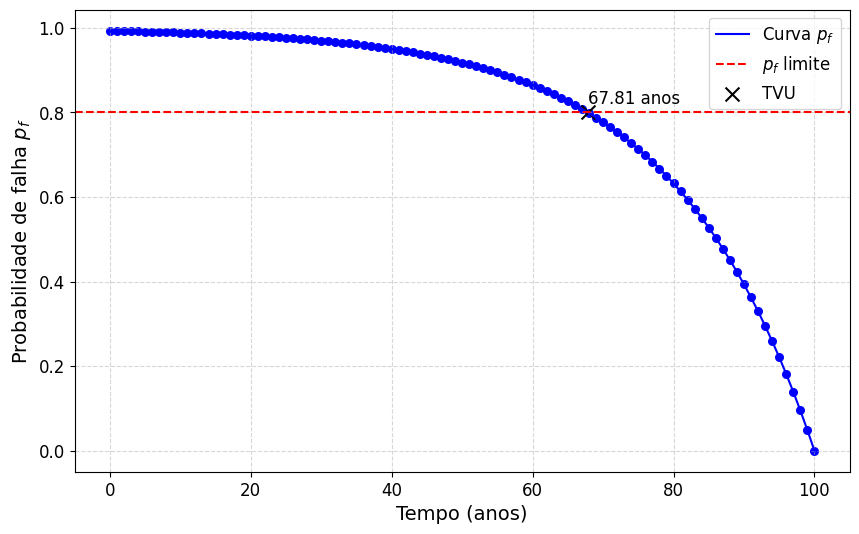
\includegraphics[width=\linewidth]{curva_tvu.png}
    \fonte{Autor (2025).}
\end{figure}

A aplicação de metodologias de predição de vida útil remanescente em estruturas de concreto traz benefícios significativos. Entre eles, destacam-se o planejamento de manutenções baseadas em condição, a redução de custos de intervenção, a gestão proativa de risco e a sustentabilidade, uma vez que se prolonga a vida útil de ativos sem comprometer a segurança estrutural.


\section{Aprendizado de Máquina} \label{AM} 

O aprendizado de máquina (AM) é um ramo da inteligência artificial que se baseia na capacidade de sistemas computacionais aprenderem padrões e relações a partir de dados, sem a necessidade de programação explícita para cada tarefa. Esse processo é matematicamente estruturado por meio do reconhecimento de padrões e da generalização a partir de exemplos, permitindo a modelagem de fenômenos complexos com alta dimensionalidade e incerteza. Dentro da engenharia civil, o uso de AM tem crescido substancialmente, sobretudo para modelar problemas estruturais que envolvem deterioração, confiabilidade e previsão de desempenho ao longo do tempo \cite{flah_machine_2021, zhang_machine_2025}.

Entre as abordagens disponíveis no campo do AM, o aprendizado supervisionado destaca-se como a mais amplamente empregada, especialmente quando há disponibilidade de dados rotulados. Nesse paradigma, um algoritmo é treinado com pares de entrada e saída conhecidos, ou seja, vetores de atributos preditivos (\textit{features}) e seus correspondentes alvos (\textit{labels}), com o objetivo de inferir uma função que relacione as variáveis de entrada ao valor de saída. Essa função aprendida é posteriormente utilizada para realizar previsões com base em novos dados, sendo útil tanto em tarefas de regressão quanto de classificação. Na prática, essa abordagem tem sido aplicada com sucesso na previsão de vida útil de materiais, detecção de danos em estruturas e avaliação da integridade estrutural \cite{flah_machine_2021, zhang_machine_2025}.

A eficácia do aprendizado supervisionado está fortemente ligada à qualidade, representatividade e volume do conjunto de dados utilizados para o treinamento. Além disso, a escolha apropriada do algoritmo de aprendizado, dos hiperparâmetros e das técnicas de regularização são essenciais para evitar fenômenos como \textit{overfitting} e \textit{underfitting}, garantindo assim a generalização adequada do modelo. Métodos como validação cruzada, análise de resíduos e testes de desempenho com dados não vistos são rotineiramente utilizados para validar e calibrar os modelos \cite{flah_machine_2021, taffese_caprm_2015}.

Na engenharia civil, os métodos de aprendizado de máquina supervisionado têm sido amplamente empregados em diferentes contextos de análise e previsão. Modelos como o \textit{Random Forest} (RF), o \textit{Gradient Boosting Machine} (GBM), o \textit{k-Nearest Neighbors} (kNN) e as \textit{Artificial Neural Networks} (ANN) destacam-se pela capacidade de estimar propriedades mecânicas de materiais, prever a durabilidade de estruturas e modelar comportamentos não lineares em sistemas físicos complexos \cite{zhang_machine_2025}. A Figura \ref{fig:modelo_ml} apresenta, de forma esquemática, as principais diferenças conceituais entre esses quatro métodos, evidenciando suas distintas abordagens de aprendizado e generalização.

\begin{figure}[H]
    \centering
    \caption{Representação esquemática das principais técnicas de aprendizado de máquina.}
    \label{fig:modelo_ml}
    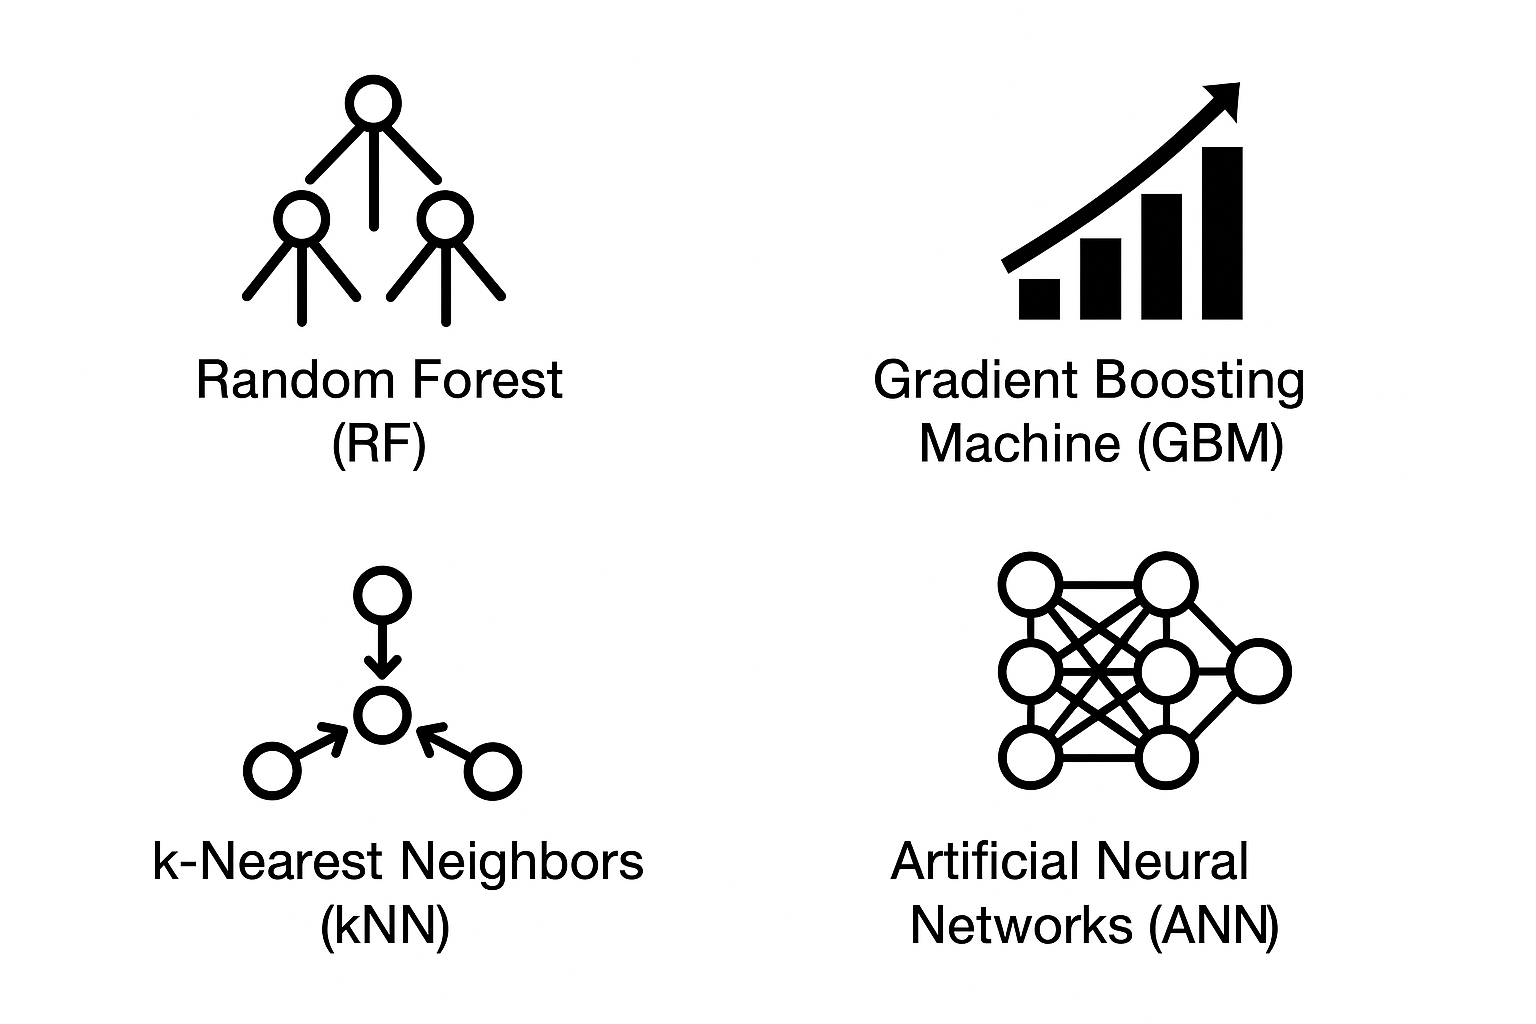
\includegraphics[width=0.7\linewidth]{modelos_ml.png}
    \fonte{Autor (2025).}
\end{figure}

O método \textit{Random Forest (RF)}, conforme descrito por \textcite{shaqadan2016}, configura-se como um modelo de conjunto (\textit{ensemble}) que integra múltiplas árvores de decisão, cada uma construída a partir de subconjuntos aleatórios dos dados. A predição final é obtida mediante a agregação das estimativas individuais das árvores, conferindo ao modelo elevada robustez frente à variabilidade e ao ruído inerentes às variáveis de entrada. Tal característica torna o \textit{RF} particularmente adequado para a análise de durabilidade de estruturas de concreto, nas quais os parâmetros físicos e mecânicos apresentam considerável heterogeneidade. Além disso, o método demanda menor esforço de pré-processamento e mantém desempenho consistente mesmo em bases de dados de grande porte.

O \textit{Gradient Boosting Machine} (GBM) adota uma estratégia sequencial (\textit{boosting}), em que múltiplos modelos simples (fracos) são treinados sucessivamente para corrigir os erros residuais do modelo anterior. Essa estratégia resulta em previsões de alta precisão, ainda que demande ajustes mais criteriosos de hiperparâmetros e maior custo computacional. Variações modernas, como \textit{XGBoost} e \textit{LightGBM}, têm se mostrado eficazes em predição de durabilidade de concreto. Estudos recentes destacam que modelos \textit{ensemble}, incluindo \textit{boosting}, figuram entre os de melhor desempenho nessa área \cite{taffese2025}.

O \textit{k-Nearest Neighbors} (kNN) baseia-se na premissa de que observações próximas no espaço de atributos tendem a apresentar resultados semelhantes. A previsão de uma nova observação é obtida com base nas amostras mais próximas, seja por média ou por voto majoritário. O kNN é simples de implementar e oferece boa interpretabilidade, pois permite identificar diretamente quais amostras contribuíram para uma determinada predição. Contudo, sua performance tende a se deteriorar em bases de dados de alta dimensionalidade ou com ruído significativo, situação comum em registros de durabilidade estrutural \cite{mandal2024}.

Por fim, as \textit{Artificial Neural Networks} (ANN) representam uma classe de modelos inspirados na estrutura de redes neurais biológicas, compostas por camadas de neurônios interconectados que aprendem representações hierárquicas e não lineares dos dados. As ANNs têm-se mostrado extremamente eficazes em problemas de previsão de durabilidade e resistência do concreto, sobretudo em situações com múltiplos atributos correlacionados e relações complexas entre variáveis \cite{taffese2025}. No entanto, exigem maior volume de dados para treinamento e apresentam menor interpretabilidade em comparação com modelos baseados em árvores.

Em síntese, as técnicas de aprendizado de máquina supervisionado, como RF, GBM, kNN e ANN, oferecem um conjunto robusto de ferramentas para a modelagem e previsão da vida útil e confiabilidade de estruturas de concreto armado. Quando integradas a análises probabilísticas e simulações estocásticas, essas metodologias possibilitam uma avaliação mais precisa do desempenho estrutural ao longo do tempo \cite{zhang_machine_2025, shaqadan2016, taffese2025, mandal2024}.

Uma das estratégias mais eficazes para gerar dados de entrada para os modelos de AM em contextos onde dados reais são escassos ou de difícil obtenção é a utilização de simulações de Monte Carlo. Esse método permite representar numericamente a variabilidade estocástica dos parâmetros envolvidos (como resistência do concreto, taxas de carbonatação e perda de seção da armadura) por meio de distribuições de probabilidade, proporcionando uma base rica e confiável para o treinamento de algoritmos supervisionados \cite{pereira_junior_reliability_2023}. A integração dessas simulações com o aprendizado supervisionado resulta em modelos híbridos que aliam precisão estatística com capacidade de predição, superando limitações de modelos puramente determinísticos.

A literatura recente reforça que a aplicação de aprendizado supervisionado em problemas estruturais não apenas complementa os modelos físicos existentes, como também amplia a capacidade analítica frente à complexidade e à incerteza envolvidas. De acordo com \textcite{zhang_machine_2025}, modelos supervisionados aplicados à confiabilidade de estruturas permitem maior precisão na previsão da vida útil e possibilitam simulações sob diferentes cenários, promovendo a tomada de decisões mais seguras e econômicas no gerenciamento de ativos. Isso é particularmente relevante no caso de estruturas expostas a ambientes agressivos, como zonas urbanas e regiões costeiras, onde a corrosão induzida por carbonatação é acelerada.

Por fim, embora o aprendizado supervisionado represente uma ferramenta poderosa para a engenharia civil, sua efetividade está condicionada ao desenvolvimento de pipelines completos de modelagem, que incluam pré-processamento adequado dos dados, tratamento de \textit{outliers}, seleção de atributos e validação estatística robusta. O avanço do campo também caminha para o uso de técnicas como aprendizado por transferência (\textit{transfer learning}) e explicabilidade de modelos (\textit{Explainable AI}), que prometem aumentar ainda mais a aplicabilidade e a confiança na adoção dessas técnicas em projetos reais \cite{flah_machine_2021, zhang_machine_2025}.

Em síntese, o aprendizado supervisionado fornece uma base sólida para o desenvolvimento de metodologias preditivas aplicadas à confiabilidade estrutural. Sua integração com simulações estocásticas, como Monte Carlo, representa uma evolução significativa nos métodos de análise de durabilidade e segurança de estruturas de concreto armado, permitindo o planejamento eficiente de ações de manutenção e reabilitação com base em dados e modelos matemáticos avançados.
\subsection{Redes Neurais Artificiais} \label{RNA}

Entre os modelos de aprendizado supervisionado, as redes neurais artificiais merecem tratamento particular neste trabalho, uma vez que constituem a camada de regressão empregada na formulação do emulador estocástico apresentada na \autoref{EMU}. As redes neurais são aproximadores universais de funções, capazes de representar mapeamentos não lineares arbitrariamente complexos desde que dotadas de capacidade suficiente \cite{goodfellow2016}. Uma rede do tipo perceptron de múltiplas camadas (\textit{Multilayer Perceptron} --- MLP) organiza-se em uma camada de entrada, uma ou mais camadas ocultas e uma camada de saída. Cada neurônio de uma camada $\ell$ computa uma combinação afim das ativações da camada anterior, seguida da aplicação de uma função de ativação não linear $\phi(\cdot)$, conforme a Equação \eqref{eq:mlp_forward}:

\begin{equation}\label{eq:mlp_forward}
\mathbf{a}^{(\ell)} = \phi\!\left(\mathbf{W}^{(\ell)} \mathbf{a}^{(\ell-1)} + \mathbf{b}^{(\ell)}\right), \qquad \mathbf{a}^{(0)} = \mathbf{z},
\end{equation}

em que $\mathbf{W}^{(\ell)}$ e $\mathbf{b}^{(\ell)}$ são, respectivamente, a matriz de pesos e o vetor de vieses da camada $\ell$, agrupados no conjunto de parâmetros $\mathbf{w} = \{\mathbf{W}^{(\ell)}, \mathbf{b}^{(\ell)}\}_\ell$, e $\mathbf{z}$ é o vetor de atributos de entrada. Funções de ativação usuais nas camadas ocultas incluem a unidade linear retificada (ReLU), $\phi(s) = \max(0,s)$, e a tangente hiperbólica, $\phi(s) = \tanh(s)$; a camada de saída, no caso de regressão, emprega tipicamente ativação linear \cite{bishop2006, goodfellow2016}.

O treinamento consiste na minimização de um funcional de perda $\mathcal{L}$ entre as saídas preditas e os valores de referência, tipicamente o erro quadrático médio, conforme a Equação \eqref{eq:ml_treinamento}:

\begin{equation}\label{eq:ml_treinamento}
\mathbf{w}^{*} = \argmin_{\mathbf{w}} \; \frac{1}{K}\sum_{k=1}^{K} \mathcal{L}\!\left(\mathbf{y}^{(k)},\, \mathcal{M}_{ML}(\mathbf{z}^{(k)};\mathbf{w})\right) + \Omega(\mathbf{w}),
\end{equation}

em que $K$ é o número de pares de treinamento $(\mathbf{z}^{(k)}, \mathbf{y}^{(k)})$, $\mathcal{M}_{ML}$ denota o modelo de regressão e $\Omega(\mathbf{w})$ é um termo de regularização que penaliza a complexidade do modelo e mitiga o sobreajuste. A minimização é conduzida por \textit{retropropagação} do gradiente combinada a um otimizador de gradiente estocástico, como o Adam. Para evitar o sobreajuste, empregam-se estratégias de regularização como parada antecipada (\textit{early stopping}), penalização $\ell_2$ dos pesos e, quando pertinente, \textit{dropout}. A partição dos dados em subconjuntos de treinamento, validação e teste, aliada a validação cruzada, sustenta a estimativa honesta do erro de generalização \cite{hastie2009}.

Cabe destacar uma particularidade da aplicação pretendida nesta dissertação: a variável-alvo da regressão não é a resposta física em si, mas os \textit{parâmetros de uma distribuição de probabilidade}. Trata-se, portanto, de um problema de regressão supervisionada de múltiplas saídas, no qual a acurácia da rede traduz-se diretamente na qualidade da distribuição emulada e, por consequência, na estimativa da probabilidade de falha e da vida útil remanescente. Essa formulação é detalhada na \autoref{EMU} e na metodologia.


\section{Emuladores Estocásticos} \label{EMU}

O elevado custo computacional de modelos de alta fidelidade frequentemente inviabiliza simulações diretas de Monte Carlo, sobretudo em análises de confiabilidade dependentes do tempo, nas quais a função de estado limite precisa ser avaliada em muitos instantes ao longo de todo o horizonte de vida útil. Esse é exatamente o caso do problema tratado nesta dissertação: a avaliação anual da margem de segurança de uma viga sujeita à carbonatação, para um número elevado de amostras e ao longo de cem anos, multiplica o número de chamadas ao simulador a ponto de tornar impraticável a varredura de cenários de inspeção e manutenção. A alternativa consagrada consiste no uso de metamodelos, também chamados de emuladores, que substituem o simulador original por uma aproximação de avaliação praticamente instantânea.

Embora os Processos Gaussianos \cite{rasmussen2006} e as Expansões em Caos Polinomial \cite{xiu2002} sejam padrão para simuladores \textit{determinísticos}, nos quais uma única avaliação caracteriza a resposta, esses metamodelos não podem ser aplicados diretamente a \textit{simuladores estocásticos}, nos quais a resposta para um mesmo vetor de entrada é uma variável aleatória cuja distribuição precisa ser caracterizada. Para esse cenário, foram propostos recentemente os emuladores estocásticos, com destaque para os modelos \textit{Generalized Lambda Models} (GLaM), nos quais a distribuição condicional da resposta é aproximada pela Distribuição Lambda Generalizada (GLD) e seus quatro parâmetros são representados por Expansão em Caos Polinomial das variáveis de entrada \cite{ZhuSudret2020, ZhuSudret2021}.

\subsection{Simuladores Estocásticos}

Matematicamente, um simulador estocástico $\mathcal{M}_S$ pode ser visto como um mapeamento que incorpora variáveis determinísticas e aleatoriedade intrínseca. Para um dado vetor de parâmetros de entrada $\mathbf{x}$ no domínio $\mathcal{D}_X$, a resposta não é um valor determinístico único, mas uma variável aleatória $Y_{\mathbf{x}}$. Essa relação é formalmente expressa pela Equação \eqref{eq:simulador_estocastico}:

\begin{equation}\label{eq:simulador_estocastico}
\mathcal{M}_S : \mathcal{D}_X \times \Omega \rightarrow \mathbb{R}, \qquad (\mathbf{x}, \omega) \mapsto \mathcal{M}_S(\mathbf{x}, \omega),
\end{equation}

em que $\mathbf{x}$ representa o conjunto de parâmetros de entrada controlados (por exemplo, geometria e propriedades dos materiais) e $\omega$ denota um evento aleatório do espaço de probabilidade $\Omega$. Essa variável latente $\omega$ introduz a estocasticidade no sistema. Consequentemente, para uma entrada fixa $\mathbf{x}$, o simulador produz uma distribuição de resultados possíveis, e não uma solução única.

No problema em estudo, $\mathcal{M}_S(\mathbf{x}, t; \omega) = g(\mathbf{x}, t; \omega)$ é a função de estado limite definida na Equação \eqref{eq:estado_limite}, e as variáveis latentes correspondem às incertezas de modelo e às flutuações ambientais e de material não explicitamente parametrizadas. Para uma mesma configuração de projeto, portanto, a resposta é uma distribuição de margens de segurança, e não um valor único --- precisamente a estrutura que motiva o uso de um emulador estocástico.

\subsection{Distribuição Lambda Generalizada}

Para capturar comportamentos probabilísticos complexos sem o custo computacional de simulações exaustivas, adota-se a Distribuição Lambda Generalizada (GLD) como núcleo do emulador estocástico. A GLD é uma família de distribuições de quatro parâmetros, altamente flexível, projetada para aproximar uma ampla gama de distribuições paramétricas \cite{KarianDudewicz2000, ZhuSudret2021}.

A GLD é definida por sua \textit{função quantílica} $Q(u)$, que é a inversa da função de distribuição acumulada, isto é, $Q(u) = F^{-1}(u)$. Essa abordagem é particularmente vantajosa para a emulação estocástica, pois facilita a amostragem por transformada inversa. Neste trabalho considera-se a família Freimer--Kollia--Mudholkar--Lin (FKML) \cite{Freimer1988}, definida pela Equação \eqref{eq:GLD_quantile}:

\begin{equation}\label{eq:GLD_quantile}
Q(u) = \lambda_1 + \frac{1}{\lambda_2} \left( \frac{u^{\lambda_3} - 1}{\lambda_3} - \frac{(1 - u)^{\lambda_4} - 1}{\lambda_4} \right)
\end{equation}

em que $u \in [0, 1]$ representa a probabilidade acumulada. A distribuição é governada por quatro parâmetros: $\lambda_1$ é o parâmetro de \textit{locação}, $\lambda_2$ é o parâmetro de \textit{escala} (com a exigência $\lambda_2 > 0$) e $\lambda_3$ e $\lambda_4$ são os parâmetros de \textit{forma}. A flexibilidade dessa parametrização permite representar distribuições simétricas e assimétricas, de caudas leves ou pesadas, o que a torna adequada à representação da margem de segurança em diferentes estágios de degradação.

\subsection{Estimação de Parâmetros pelo Método dos Momentos}

Para calibrar o emulador GLD, os quatro parâmetros $\boldsymbol{\lambda} = \{\lambda_1, \dots, \lambda_4\}$ devem ser estimados a partir de um conjunto de avaliações do modelo \cite{karian2010handbook, corlu2016}. Neste trabalho, emprega-se o \textit{Método dos Momentos} \cite{lakhany2000}, que consiste em igualar os momentos teóricos da GLD aos momentos empíricos calculados do conjunto amostral $\mathcal{Y} = \{y^{(1)}, \dots, y^{(N)}\}$. Os quatro primeiros momentos --- média $\mu$, variância $\sigma^2$, assimetria $\delta$ e curtose $\kappa$ --- relacionam-se analiticamente aos parâmetros $\boldsymbol{\lambda}$ conforme as Equações \eqref{eq:mean} a \eqref{eq:kurt}:

\begin{equation}\label{eq:mean}
\mu = \lambda_1 - \frac{1}{\lambda_2} \left( \frac{1}{\lambda_3 + 1} - \frac{1}{\lambda_4 + 1} \right)
\end{equation}

\begin{equation}\label{eq:var}
\sigma^2 = \frac{v_2 - v_1^2}{\lambda_2^2}
\end{equation}

\begin{equation}\label{eq:skew}
\delta = \frac{v_3 - 3v_1v_2 + 2v_1^3}{(v_2 - v_1^2)^{3/2}}
\end{equation}

\begin{equation}\label{eq:kurt}
\kappa = \frac{v_4 - 4v_1v_3 + 6v_1^2v_2 - 3v_1^4}{(v_2 - v_1^2)^2}
\end{equation}

Nessas expressões, $v_k$ denota uma função não linear que depende apenas de $\lambda_3$ e $\lambda_4$, dada pela Equação \eqref{eq:vk}, em que $B(\cdot, \cdot)$ representa a função Beta:

\begin{equation}\label{eq:vk}
v_k = \sum_{j=0}^{k} \frac{(-1)^j}{\lambda_3^{k-j} \lambda_4^j} \binom{k}{j} B\!\left(\lambda_3(k-j) + 1,\; \lambda_4 j + 1\right)
\end{equation}

A calibração dos parâmetros da GLD é, portanto, formulada como um problema inverso, cujo objetivo é minimizar a discrepância entre os momentos analíticos (Equações \eqref{eq:mean} a \eqref{eq:kurt}) e os momentos empíricos derivados do simulador estocástico. Para resolver esse sistema não linear, emprega-se o algoritmo de otimização Broyden--Fletcher--Goldfarb--Shanno (BFGS) \cite{nocedal2006}, um método quase-Newton adequado a esse tipo de estimação devido ao tratamento eficiente de gradientes e às boas propriedades de convergência em espaços multidimensionais. O procedimento numérico foi implementado no PyGLAM, biblioteca em linguagem Python desenvolvida no âmbito deste trabalho especificamente para a emulação de simuladores estocásticos com Distribuições Lambda Generalizadas \cite{pyglam2025}.

Cabe registrar que o arcabouço GLaM original \cite{ZhuSudret2021} emprega máxima verossimilhança condicional combinada a mínimos quadrados generalizados para a estimação dos parâmetros, dispensando réplicas no plano de experimentos. A opção pelo Método dos Momentos com réplicas adotada nesta dissertação justifica-se por três razões: pela robustez e simplicidade de implementação; pelo baixo custo de cada avaliação dos modelos mecânicos aqui considerados, que torna as réplicas viáveis; e pelo controle direto da qualidade do ajuste local em cada ponto do plano de experimentos, requisito importante para a camada temporal descrita na metodologia.

A Figura \ref{fig:pyglam_fits} apresenta exemplos de ajuste da GLD a distribuições tradicionais --- Normal, Gumbel e Uniforme --- obtidos com o PyGLAM, evidenciando a capacidade da família FKML de reproduzir formas distribucionais bastante distintas com um único conjunto de quatro parâmetros.

\begin{figure}[H]
    \centering
    \caption{Ajuste do emulador GLD a diferentes distribuições-alvo.}
    \label{fig:pyglam_fits}
    \begin{subfigure}[b]{0.32\textwidth}
        \centering
        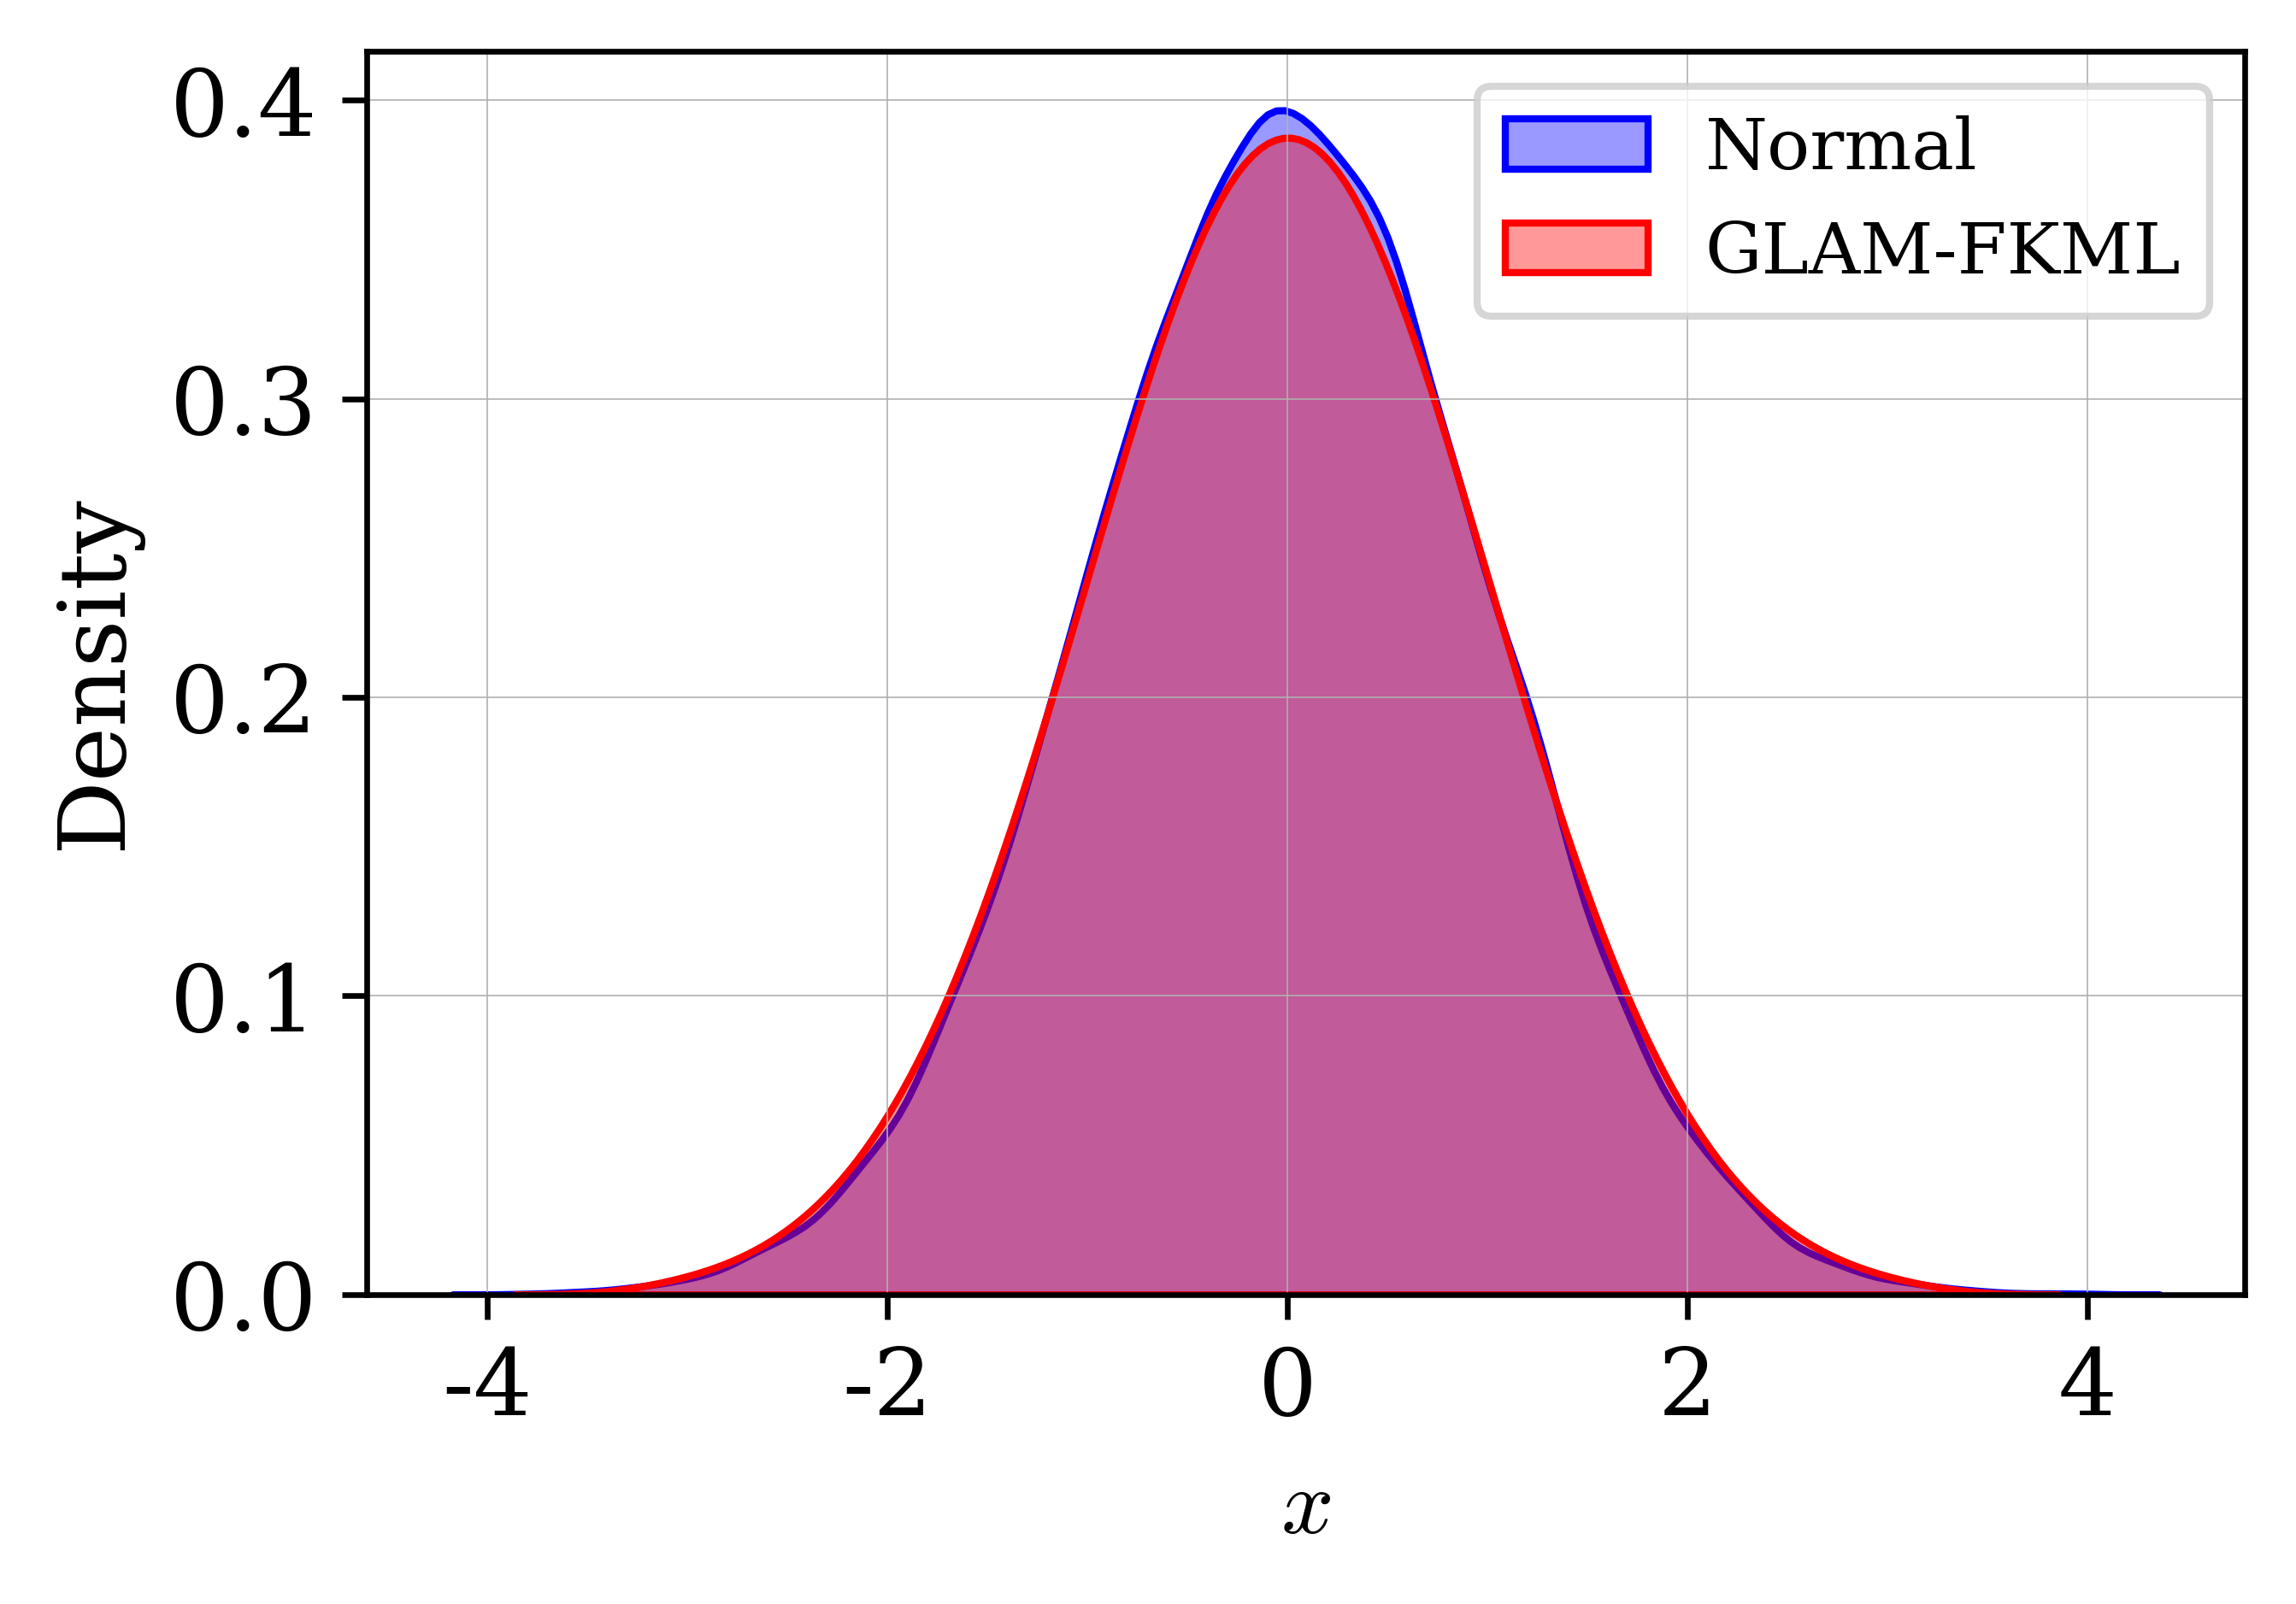
\includegraphics[width=\textwidth]{z_kde_histogram_compare.png}
        \caption{Normal}
        \label{fig:fit_normal}
    \end{subfigure}
    \hfill
    \begin{subfigure}[b]{0.32\textwidth}
        \centering
        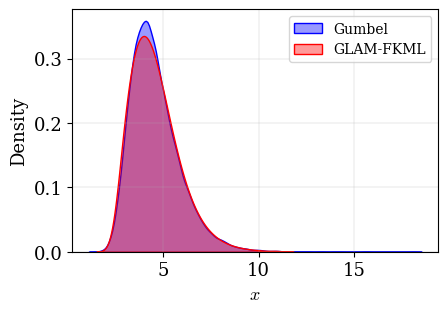
\includegraphics[width=\textwidth]{z_fig_gumbel.png}
        \caption{Gumbel}
        \label{fig:fit_gumbel}
    \end{subfigure}
    \hfill
    \begin{subfigure}[b]{0.32\textwidth}
        \centering
        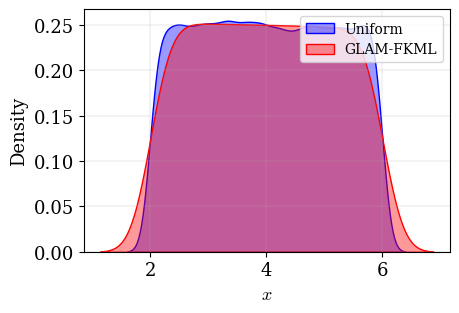
\includegraphics[width=\textwidth]{z_fig_uniform.png}
        \caption{Uniforme}
        \label{fig:fit_uniform}
    \end{subfigure}
    \vspace{0.2cm}
    \fonte{Autor (2025).}
\end{figure}

\subsection{Acoplamento com a Expansão em Caos Polinomial}

Seguindo a metodologia proposta por \textcite{ZhuSudret2021}, a GLD é acoplada à Expansão em Caos Polinomial (PCE) para a construção de um emulador global. Nesse arcabouço, a resposta estocástica do simulador para qualquer entrada $\mathbf{X}$ é modelada por uma GLD cujos parâmetros $\boldsymbol{\lambda}$ são, eles próprios, funções das variáveis de entrada.

Dado um conjunto de parâmetros de entrada $\mathbf{X}$ governado por uma função densidade de probabilidade conjunta $f_{\mathbf{X}}(\mathbf{x})$, cada componente do vetor de parâmetros $\lambda_i$ é aproximada por uma PCE truncada, conforme a Equação \eqref{eq:pce_lambda}:

\begin{equation}\label{eq:pce_lambda}
\lambda_i(\mathbf{X}) \approx \sum_{\boldsymbol{\alpha} \in \mathcal{A}} a_{i, \boldsymbol{\alpha}} \Psi_{\boldsymbol{\alpha}}(\mathbf{X}), \quad i = \{1, 2, 3, 4\}
\end{equation}

em que $\Psi_{\boldsymbol{\alpha}}(\mathbf{X})$ são polinômios ortonormais multivariados específicos das distribuições de entrada \cite{xiu2002}, $a_{i, \boldsymbol{\alpha}}$ são os coeficientes a determinar e $\mathcal{A}$ é o conjunto de multi-índices que define o esquema de truncamento, usualmente uma base de grau total \cite{blatman2011}.

Uma vez estimados os coeficientes, o emulador PCE--GLD fornece instantaneamente a distribuição de probabilidade completa, por meio dos parâmetros $\boldsymbol{\lambda}$, para qualquer nova entrada $\mathbf{X}^*$, sem exigir novas execuções do simulador estocástico original. Uma vantagem adicional do acoplamento com a PCE é que os índices de sensibilidade de Sobol podem ser obtidos analiticamente a partir dos coeficientes da expansão \cite{sudret2008}, permitindo quantificar, sem custo adicional, a contribuição de cada variável de entrada para a variância da resposta.

\subsection{Extensão ao Domínio Temporal}

O arcabouço PCE--GLD descrito nas seções anteriores é formulado para um instante fixo. Como o processo de carbonatação é inerentemente dependente do tempo, a aplicação pretendida nesta dissertação exige que a evolução da distribuição da margem de segurança seja capturada ao longo de toda a vida em serviço da estrutura. Propõe-se, para tanto, a extensão do arcabouço por meio de uma camada de regressão que recebe o tempo como variável de entrada contínua.

Nessa formulação, os parâmetros $\boldsymbol{\lambda}$ da GLD são avaliados em passos de tempo discretos e um modelo de aprendizado de máquina de múltiplas saídas --- a rede neural artificial descrita na \autoref{RNA} --- é subsequentemente treinado para mapear o espaço conjunto de variáveis físicas e tempo nos parâmetros da distribuição, atuando como interpolador contínuo entre os instantes efetivamente simulados. O procedimento concreto de construção desse emulador, incluindo o plano de experimentos, o número de réplicas e as métricas de validação adotadas, é detalhado no capítulo de metodologia.

	
	% 3 - Metodologia
	\chapter{Metodologia} \label{met}

Este capítulo apresenta o procedimento adotado para a obtenção dos resultados da presente dissertação, cujo objetivo consiste em aplicar uma análise do tempo de vida útil remanescente de uma estrutura de concreto armado sujeita à carbonatação. O método proposto foi desenvolvido de forma a integrar modelagem computacional, simulação estocástica e aprendizado de máquina, com o propósito de avaliar o desempenho estrutural de maneira probabilística ao longo do tempo.

A metodologia está organizada em duas frentes complementares. A primeira, já implementada e cujos resultados são apresentados no \autoref{cap:resultados}, compreende a construção do banco de dados sintético por simulação de Monte Carlo com Hipercubo Latino e o treinamento de modelos de regressão supervisionada para a predição direta do tempo de vida útil. A segunda frente, em desenvolvimento, substitui a predição pontual do tempo de vida útil pela emulação da \textit{distribuição condicional completa} da função de estado limite ao longo do tempo, por meio do emulador estocástico PCE--GLD acoplado a uma camada temporal de aprendizado de máquina. Essa segunda frente é o que permite derivar, além do tempo médio de falha, a distribuição probabilística da vida útil remanescente e as métricas de risco associadas.

\section{Desenvolvimento do Banco de Dados}

Por meio de programação em Python, será elaborado um banco de dados abrangente contendo diversos modelos de vigas de concreto armado tradicionalmente empregadas em edificações. A metodologia adota um delineamento fatorial completo para considerar todas as combinações das variáveis de interesse. Os parâmetros utilizados para criação desse banco de dados são: (\textit{i}) largura da seção transversal ($b_w$) entre 14 e 30 cm; (\textit{ii}) altura da seção ($h$) entre 30 e 70 cm; (\textit{iii}) resistência característica do concreto ($f_{ck}$) entre 20 e 50 MPa; e (\textit{iv}) taxa de armadura ($A_s$) entre 0,15\% e 1,50\%, intervalo que permite apenas vigas com armadura simples, ou seja, sem armadura dupla. Esse delineamento fatorial completo resultará em cerca de 3600 vigas de concreto armado.

Para a determinação do momento solicitante, inicialmente será calculado o momento resistente limite, com o objetivo de avaliar a capacidade máxima de resistência das vigas-modelo, conforme apresentado na Equação \eqref{eq:mrd_lim}. Em seguida, o momento total será decomposto em momento permanente ($M_{gk}$) e momento variável ($M_{qk}$), de acordo com os modelos de participação do carregamento descritos nas Equações \eqref{eq:mgk} e \eqref{eq:mqk}. Os fatores parciais de segurança adotados serão $\gamma_g = 1.30$ para as ações permanentes e $\gamma_q = 1.40$ para as ações variáveis. 

\begin{equation}
M_{gk} = \frac{M_{Rd,lim}}{\gamma_g + \gamma_q \cdot \frac{\chi}{(1 - \chi)}}
\label{eq:mgk}
\end{equation}

\vspace{6pt}

\begin{equation}
M_{qk} = \frac{M_{Rd,lim}}{\gamma_g \cdot \frac{(1 - \chi)}{\chi} + \gamma_q}
\label{eq:mqk}
\end{equation}

O cálculo da área de aço ($A_s$) de cada viga será realizado por meio da Equação \eqref{eq:a_s}. Em seguida, será determinada a taxa de armadura ($\rho_s$), conforme a Equação \eqref{eq:rho_s}.

\begin{equation}\label{eq:a_s}
A_s = \frac{M_{Sd}}{z \cdot f_{yd}}
\end{equation}

\begin{equation}
z = d - 0{,}5\,\lambda 
\bigg(
    \frac{d - \sqrt{d^{2} - 2
    \left(
        \dfrac{M_{sd}}{b_w\,\alpha_c\,\dfrac{f_{ck}}{\gamma_c}}
    \right)
    }}{\lambda}
\bigg)
\label{eq:braco_z}
\end{equation}

\begin{equation}\label{eq:rho_s}
\rho_s = \frac{A_s}{A_c} \cdot 100
\end{equation}

% \begin{table}[hptb!]
% \centering
% \caption{Estatísticas descritivas das variáveis do conjunto de dados}
% \label{tab:dados_banco}
% \begin{tabular}{l p{6cm} c c c c}
% \toprule
% \textbf{Variável} & \textbf{Descrição} & \textbf{Média} & \textbf{Desv. Padrão} & \textbf{Mínimo} & \textbf{Máximo} \\ 
% \midrule
% $b_w$ (m)       & Largura útil da seção transversal & 0,2450 & 0,0743 & 0,1400 & 0,3500 \\
% $h$ (m)         & Altura da seção transversal & 0,5000 & 0,1414 & 0,3000 & 0,7000 \\
% $f_{ck}$ (MPa)  & Resistência característica do concreto à compressão & 35\,000 & 10\,608,30 & 20\,000 & 50\,000 \\
% $M_{gk}$ (kN·m) & Momento fletor devido às ações permanentes & 111,38 & 107,03 & 2,81 & 890,01 \\
% $M_{qk}$ (kN·m) & Momento fletor devido às ações variáveis & 59,97 & 66,99 & 0,70 & 593,34 \\
% $A_s$ (m²)      & Área de armadura de tração & 0,0012 & 0,0009 & 0,0001 & 0,0055 \\
% \bottomrule
% \end{tabular}
% \fonte{Autor (2025).}
% \end{table}

% As médias dos parâmetros geométricos $b_w$ (largura da seção) e $h$ (altura da seção) serão, respectivamente, de 0,24 m e 0,50 m. A resistência à compressão do concreto ($f_{ck}$) apresentará média de 35.000 kPa, com valores variando entre 20.000 e 50.000 kPa. As variáveis relacionadas às ações apresentarão maior variabilidade. O momento característico das cargas permanentes ($M_{gk}$) variará entre 2,81 e 890,02 kN·m, com média de 111,38 kN·m e intervalo interquartil (IQR) de 108,90 kN·m. De forma análoga, o momento característico das cargas variáveis ($M_{qk}$) variará entre 0,70 e 593,34 kN·m, apresentando média de 59,97 kN·m e IQR de 61,30 kN·m.

\section{Aplicação de Técnicas de Amostragem }

Após a construção do banco de dados, será realizada uma simulação estocástica da viga, com o objetivo de representar o comportamento temporal da função de estado limite, expressa pela Equação \eqref{eq:estado_limite}. As variáveis aleatórias consideradas, bem como suas respectivas fontes bibliográficas, serão apresentadas na Tabela \ref{tab:estatisticas_vars}. 

\begin{equation}\label{eq:estado_limite}
g = 
\begin{cases}
E_r \cdot M_{rd} - E_s \cdot M_{sd}, & \text{se } y(t) < \text{cobrimento} \\
E_r \cdot M_{rd,cor} - E_s \cdot M_{sd}, & \text{se } y(t) \geq \text{cobrimento}
\end{cases}
\end{equation}

A equação \eqref{eq:estado_limite} define a função de estado limite empregada na verificação da confiabilidade estrutural. Essa função expressa a diferença entre a resistência estrutural disponível e a solicitação atuante, sendo a condição de falha caracterizada quando o valor de $g$ torna-se negativo ($g < 0$). A formulação contempla duas situações distintas: a primeira, correspondente à fase em que o processo de corrosão por carbonatação ainda não atingiu a armadura; e a segunda, referente ao estágio em que a frente de carbonatação alcança o cobrimento e inicia a deterioração da armadura. Dessa forma, o modelo incorpora a influência do tempo e o consequente decréscimo da resistência, representado pela profundidade de carbonatação $y(t)$.

As variáveis que compõem a equação \eqref{eq:estado_limite} são definidas da seguinte forma:
$g$ representa a função de estado limite, cuja condição de falha ocorre quando $g < 0$;
$E_r$ corresponde ao erro de modelo referente à resistência do sistema estrutural;
$E_s$ refere-se ao erro de modelo referente às solicitações aplicadas;
$M_{rd}$ indica o momento resistente da seção transversal não degradada;
$M_{rd,cor}$ representa o momento resistente da seção degradada pela corrosão;
$M_{sd}$ é o momento solicitante de cálculo;
$y(t)$ expressa a profundidade de carbonatação em função do tempo;
e o \textit{cobrimento} corresponde à espessura da camada de concreto que protege a armadura.

\begin{table}[H]
\centering
\footnotesize
\caption{Parâmetros estatísticos das variáveis básicas}
\label{tab:estatisticas_vars}
\begin{tabularx}{\textwidth}{
    p{2.2cm}   % 1ª coluna (Descrição)
    p{1.5cm}     % 2ª coluna (Notação)
    c          % 3ª (Distribuição)
    p{1.5cm}          % 4ª (Média)
    p{2.0cm}     % 5ª (C.O.V.)
    X          % 6ª (Referência, ajusta automaticamente)
}
\toprule
\textbf{Descrição} & \textbf{Notação} & \textbf{Distribuição} & \textbf{Média} & \textbf{C.O.V.} & \textbf{Referência} \\ 
\midrule
Carga permanente & $M_{gk}$ (kN·m) & Normal & $1{,}06 \, M_{gk}$ & 0,12 & \cite{pereira_junior_reliability_2023,costa_probabilistic_2023} \\ 
Carga variável & $M_{qk}$ (kN·m) & Gumbel & $0{,}21 \, M_{qk}$ & 0,76 & \cite{costa_probabilistic_2023} \\ 
Resistência do concreto & $f_{ck}$ (MPa) & Normal & $1{,}22 \, f_c$ & 0,15 & \cite{pereira_junior_reliability_2023,costa_probabilistic_2023} \\ 
Resistência do aço & $f_{yk}$ (MPa) & Normal & $1{,}22 \, f_y$ & 0,04 & \cite{pereira_junior_reliability_2023,costa_probabilistic_2023} \\ 
Humidade & $u_r$ (\%) & Lognormal & 57,25 & 0,26 (a=2,94,b=2,21) & Trabalho presente \\ 
Temperatura & $T$ (°C) & Lognormal & 21,10 & 0,03 & Trabalho presente \\ 
Perda de seção por corrosão & $i_{cor 20}$ ($\mu$A/cm²) & Lognormal & 0,431 & 0,259 & \cite{peng_climate_2016} \\ 
Erro de modelo da resistência & $E_r$ & Lognormal & 1,00 & 0,05 & \cite{santos_reliability_2014} \\ 
Erro de modelo da solicitação & $E_s$ & Lognormal & 1,00 & 0,05 & \cite{santos_reliability_2014} \\ 
\bottomrule
\end{tabularx}
\fonte{Autor (2025).}
\end{table}

A Tabela \ref{tab:estatisticas_vars} apresenta os parâmetros estatísticos adotados para as variáveis básicas utilizadas na análise de confiabilidade. As variáveis consideradas incluem ações permanentes e variáveis, propriedades mecânicas dos materiais (concreto e aço), além de fatores ambientais e de incerteza. As distribuições probabilísticas foram definidas com base em estudos anteriores, e recomendações da literatura indicadas, de modo a representar adequadamente a variabilidade de cada parâmetro. Observa-se que as resistências do concreto e do aço seguem distribuições normais, enquanto as variáveis associadas ao ambiente e aos erros de modelo são descritas por distribuições lognormais. Os coeficientes de variação (C.O.V.) indicam o grau de dispersão de cada variável em relação à sua média, sendo que valores mais elevados, como o da carga variável, refletem maior incerteza.


\section{Determinação da Vida Útil Remanescente Com Aplicação do Aprendizado de Máquina}

Por fim, para a estimativa do tempo de vida útil remanescente, será desenvolvido um modelo de aprendizado de máquina voltado à análise de séries temporais. Serão empregados métodos baseados em regressão, conforme descrito na \autoref{AM}. Na aplicação do modelo temporal à previsão da equação de estado limite, será incorporado o conceito de \textit{lag}, o qual se fundamenta na premissa de que o valor no pseudo-tempo $t$ é influenciado pelos estados anteriores, em especial por $t-1$. Nesta pesquisa, a série temporal será delimitada a um horizonte de 100 anos, representando o ciclo de vida estrutural considerado para as análises.

As métricas de avaliação de desempenho dos modelos de aprendizado de máquina são fundamentais para quantificar a precisão das previsões e a capacidade de generalização do modelo. No presente trabalho, serão utilizadas quatro métricas amplamente reconhecidas na literatura para problemas de regressão: a raiz do erro quadrático médio (RMSE), o coeficiente de determinação ($R^2$), o erro percentual médio absoluto (MAPE) e o índice de acurácia dentro de 10\% (A10). Cada uma dessas métricas permite avaliar o desempenho sob diferentes perspectivas, considerando tanto a dispersão dos erros quanto a capacidade do modelo de reproduzir os valores observados.

A métrica RMSE (\textit{Root Mean Squared Error}) medirá a magnitude média dos erros entre os valores previstos e os observados, penalizando de forma mais intensa os erros de maior amplitude. Sua formulação é dada pela Equação \eqref{eq:rmse}:

\begin{equation}
\mathrm{RMSE} = \sqrt{ \frac{1}{N} \sum_{i=1}^{N} (y_i - \hat y_i)^2 }
\label{eq:rmse}
\end{equation}

em que $N$ representa o número total de observações (adimensional), $y_i$ é o valor observado da variável dependente e $\hat{y}_i$ é o valor previsto pelo modelo, ambos expressos na mesma unidade de medida. O RMSE é expresso nas mesmas unidades da variável predita e reflete a dispersão média dos resíduos em torno da linha de regressão. Valores menores de RMSE indicam melhor desempenho preditivo \cite{montgomery_design_2020, nguyen_prediction_2022}.

O coeficiente de determinação ($R^2$) expressará a proporção da variância total dos dados explicada pelo modelo, sendo uma medida global de ajuste. Sua definição é dada pela Equação \eqref{eq:r2}:

\begin{equation}
R^2 = 1 - \frac{ \sum_{i=1}^{N} (y_i - \hat y_i)^2 }{ \sum_{i=1}^{N} (y_i - \overline{y})^2 }
\label{eq:r2}
\end{equation}

em que $\overline{y}$ representa a média dos valores observados ($\overline{y} = \frac{1}{N}\sum_{i=1}^{N} y_i$). Valores de $R^2$ próximos de 1 indicam elevada capacidade explicativa do modelo, enquanto valores próximos de 0 indicam baixo poder de previsão. Em modelos não lineares ou com ajustes forçados, é possível obter valores negativos de $R^2$ \cite{montgomery_design_2020, nguyen_prediction_2022}.

O erro percentual médio absoluto (MAPE, \textit{Mean Absolute Percentage Error}) medirá o erro médio relativo entre as previsões e os valores reais, sendo amplamente utilizado por permitir comparação entre variáveis de diferentes escalas \cite{nguyen_prediction_2022}. É definido pela Equação \eqref{eq:mape}:

\begin{equation}
\mathrm{MAPE} = \frac{100}{N} \sum_{i=1}^{N} \left| \frac{y_i - \hat{y}_i}{y_i} \right|
\label{eq:mape}
\end{equation}

em que $N$, $y_i$ e $\hat{y}_i$ mantêm as definições anteriores. O resultado é expresso em percentual e valores menores de MAPE indicam maior precisão do modelo. Segundo \textcite{de_myttenaere_mean_2016}, valores de MAPE inferiores a 10\% geralmente indicam excelente desempenho preditivo.

O índice de acurácia de 10\% (A10) quantificará a proporção de previsões cujo erro relativo é inferior a 10\% em relação ao valor real, fornecendo uma interpretação intuitiva da precisão do modelo. A métrica é definida pela Equação \eqref{eq:a10}:

\begin{equation}
\mathrm{A10} = \frac{1}{N} \sum_{i=1}^{N} \mathbb{I}\left( \left| \frac{y_i - \hat{y}_i}{y_i} \right| \le 0{,}10 \right)
\label{eq:a10}
\end{equation}

em que $\mathbb{I}(\cdot)$ é a função indicadora, que assume valor 1 se a condição for verdadeira e 0 caso contrário. O índice A10 varia de 0 a 1, representando, respectivamente, ausência total e acurácia perfeita. Essa métrica tem sido recomendada para a análise de previsões contínuas por permitir interpretação direta da proporção de acertos \cite{nguyen_prediction_2022}.

O modelo de análise que será desenvolvido adota uma base de dados anual, de modo que os valores da função de estado limite serão anualizados para representar adequadamente a evolução do desempenho estrutural ao longo do tempo. Para o conjunto de treinamento do modelo, será utilizada a divisão padrão de 70\% dos dados para treino e 30\% para teste da série temporal, assegurando a validação da capacidade preditiva do algoritmo. 

Ao final, com o modelo de predição devidamente treinado e validado, será possível definir um tempo de inspeção ($t_{insp}$) arbitrário e, a partir dessa informação, estimar a vida útil remanescente da estrutura correspondente à condição de degradação observada.

Como diversas amostras da curva serão realizadas o valor médio será utilizado para previsão com o modelo de IA. A partir desse modelo os tempos de inspeção poderão ser indicados e então o tempo de vida útil remanescente poderá ser estimado.

As principais técnicas de aprendizado de máquina abordadas neste trabalho baseiam-se, direta ou indiretamente, na lógica de árvores de regressão. Dessa forma, apresenta-se a seguir uma breve descrição desse mecanismo. Conforme \textcite{Cruvinel2024ConcreteAI}, uma árvore de decisão para regressão realiza particionamentos sucessivos no conjunto de dados, com o objetivo de reduzir a variabilidade interna de cada região resultante. Em cada nó $m$, seleciona-se o atributo $j$ e o limiar $t_m$ que melhor dividem o conjunto $(x, y)$ em dois subconjuntos distintos:

\[
Q_m^{left}(j,t_m) = \{ (x, y) \mid x_j \le t_m \}
\]

\[
Q_m^{right}(j,t_m) = \{ (x, y) \mid x_j > t_m \}
\]

A função de custo a ser minimizada para a melhor divisão $\theta$ é:

\[
Loss(Q_m, \theta) =
\frac{n_m^{left}}{n_m} H(Q_m^{left}) +
\frac{n_m^{right}}{n_m} H(Q_m^{right})
\]

onde:

\[
H(Q_m) = \frac{1}{n_m} \sum_{y \in Q_m} (y - \bar{y}_m)^2
\]

e a previsão no nó é dada pela média dos valores alvo:

\[
\bar{y}_m = \frac{1}{n_m} \sum_{y \in Q_m} y
\]

Assim, o modelo procura reduzir a variância dentro de cada região a
cada divisão do conjunto de dados. A árvore prossegue particionando os
dados até atingir um critério de parada, como profundidade máxima ou
número mínimo de amostras.














\section{Construção do Emulador Estocástico Dependente do Tempo}
\label{sec:construcao_emulador}

Definidos o simulador estocástico, representado pela função de estado limite da Equação \eqref{eq:estado_limite}, e o núcleo estatístico do emulador, apresentado na \autoref{EMU}, descreve-se nesta seção o procedimento de construção do emulador PCE--GLD e sua extensão ao domínio temporal.

\subsection{Plano de Experimentos e Ajuste Local}

O treinamento do emulador PCE--GLD segue as etapas descritas a seguir:

\begin{alineas}
    \item \textbf{Plano de experimentos:} um conjunto de $M$ pontos amostrais $\{\mathbf{x}^{(1)}, \dots, \mathbf{x}^{(M)}\}$ é gerado por Amostragem por Hipercubo Latino, conforme o procedimento já descrito no \autoref{cap:referencial} \cite{mckay_comparison_1979};
    \item \textbf{Avaliações estocásticas:} para cada ponto $\mathbf{x}^{(j)}$, o simulador estocástico original é executado $N$ vezes, gerando um conjunto amostral local da resposta, $\mathcal{Y}^{(j)}$;
    \item \textbf{Ajuste local da GLD:} o Método dos Momentos, implementado no PyGLAM com o otimizador BFGS, é utilizado para estimar os parâmetros locais ótimos $\hat{\boldsymbol{\lambda}}^{(j)}$ para cada conjunto $\mathcal{Y}^{(j)}$;
    \item \textbf{Estimação dos coeficientes da PCE:} a partir dos pares $\{\mathbf{x}^{(j)}, \hat{\boldsymbol{\lambda}}^{(j)}\}_{j=1}^{M}$, os coeficientes $a_{i, \boldsymbol{\alpha}}$ da Equação \eqref{eq:pce_lambda} são calculados para cada parâmetro $\lambda_i$.
\end{alineas}

\subsection{Emulação Dependente do Tempo}

A base de treinamento do emulador temporal é construída avaliando-se o simulador estocástico em $N_t$ passos de tempo discretos $\{t_1, t_2, \dots, t_{N_t}\}$. Para cada passo $t_m$, um conjunto de $M$ amostras do vetor de entrada $\mathbf{x}^{(j)}$ é avaliado, produzindo os parâmetros locais correspondentes $\hat{\boldsymbol{\lambda}}^{(j, m)}$ via PyGLAM. A base de dados resultante $\mathcal{D}$ é definida pela Equação \eqref{eq:dataset_temporal}:

\begin{equation}\label{eq:dataset_temporal}
\mathcal{D} = \left\{ \left( \mathbf{x}^{(j)}, t_m \right), \hat{\boldsymbol{\lambda}}^{(j, m)} \right\}, \quad j=1,\dots,M \;\text{ e }\; m=1,\dots,N_t
\end{equation}

Para prever os parâmetros da GLD em um instante arbitrário $t^{*}$, emprega-se o modelo de aprendizado de máquina de múltiplas saídas descrito na \autoref{RNA}, que aprende o mapeamento não linear $f: (\mathbf{X}, t) \to \mathbb{R}^4$, conforme a Equação \eqref{eq:ml_temporal}:

\begin{equation}\label{eq:ml_temporal}
\hat{\boldsymbol{\lambda}}(\mathbf{X}, t) \approx \mathcal{M}_{ML}(\mathbf{X}, t; \mathbf{w})
\end{equation}

Ao incluir o passo de tempo como entrada explícita, o emulador interpola os valores de $\{\lambda_1, \dots, \lambda_4\}$ entre os anos simulados, fornecendo uma evolução contínua da distribuição da margem de segurança ao longo de todo o período de análise. Duas salvaguardas são adotadas na implementação. A primeira consiste em impor a restrição de validade $\lambda_2 > 0$ na saída do regressor, o que assegura que toda predição corresponda a uma GLD bem definida; adota-se, para tanto, a predição do logaritmo do parâmetro de escala, com posterior exponenciação. A segunda consiste em permitir que parâmetros que exibam baixa sensibilidade às entradas sejam excluídos do treinamento e representados por seu valor médio, decisão tomada caso a caso a partir de análise exploratória, conforme discutido no \autoref{cap:resultados}.

\subsection{Métricas de Validação do Emulador}
\label{sec:metricas_emulador}

A similaridade estatística entre os dados de referência, obtidos por simulação direta de Monte Carlo, e as amostras geradas pelo emulador é avaliada por um conjunto complementar de métricas, todas aplicadas em pontos e instantes \textit{não utilizados no treinamento}. Cabe observar que essas métricas são de natureza distinta daquelas apresentadas na seção anterior: enquanto RMSE, $R^2$, MAPE e A10 medem a acurácia de uma predição pontual, as métricas descritas a seguir medem a aderência entre \textit{distribuições}.

\subsubsection{Testes de aderência}

O teste de Kolmogorov--Smirnov \cite{massey1951} quantifica a máxima distância entre as funções de distribuição acumuladas empíricas, sendo sensível a discrepâncias globais. O teste de Anderson--Darling \cite{anderson1952, scholz1987}, por sua vez, pondera fortemente as caudas, sendo adequado para detectar desvios nas regiões extremas, justamente as mais relevantes para a análise de confiabilidade.

\subsubsection{Comparação de quantis}

Os erros relativos nos quantis $\{0{,}001;\, 0{,}01;\, 0{,}5;\, 0{,}99;\, 0{,}999\}$ localizam a origem de eventuais discrepâncias e quantificam diretamente a qualidade da aproximação na cauda inferior, região que governa a probabilidade de falha. Trata-se da métrica mais informativa para o presente problema, pois um emulador pode apresentar excelente ajuste global e, ainda assim, falhar precisamente na região que determina $p_f$.

\subsubsection{Divergência de Kullback--Leibler}

Para duas densidades $p(x)$, de referência, e $q(x)$, do emulador, a entropia relativa \cite{kullback1951, cover2006} é definida pela Equação \eqref{eq:kl_continua}:

\begin{equation}\label{eq:kl_continua}
D(p \,\|\, q) = \int p(x)\, \log \frac{p(x)}{q(x)}\, dx
\end{equation}

Essa medida é não negativa e anula-se se, e somente se, $p = q$. Embora não seja simétrica nem satisfaça a desigualdade triangular, é frequentemente útil interpretá-la como uma medida de ``distância'' entre distribuições, fornecendo um escalar global de qualidade do emulador.

\section{Da Distribuição Emulada à Vida Útil Remanescente}
\label{sec:emulador_rul}

Esta seção estabelece a ponte entre a distribuição condicional de $g(\mathbf{X},t)$ fornecida pelo emulador e as grandezas de interesse para a gestão de ativos: a probabilidade de falha dependente do tempo, a distribuição do tempo até a falha, a vida útil remanescente probabilística e suas métricas de risco.

\subsection{Probabilidade de Falha e Função de Confiabilidade}

Dado que o emulador fornece, para qualquer instante $t$, os parâmetros $\hat{\boldsymbol{\lambda}}(\mathbf{X},t)$ da GLD que aproxima a distribuição de $g$, a probabilidade de falha instantânea é obtida diretamente da função quantílica, sem necessidade de amostragem, conforme a Equação \eqref{eq:pf_t}:

\begin{equation}\label{eq:pf_t}
p_f(t) = P\left[\, g(\mathbf{X}, t) \leq 0 \,\right] = F_{g(t)}(0) = Q^{-1}_{t}(0)
\end{equation}

em que $F_{g(t)}$ é a função de distribuição acumulada da margem de segurança no instante $t$ e $Q_t$ a correspondente função quantílica emulada. O índice de confiabilidade generalizado associado é obtido pela Equação \eqref{eq:beta}, já apresentada. A função de confiabilidade da estrutura, entendida como a probabilidade de sobrevivência até $t$, é denotada $R(t)$; para processos de degradação monotônica, como a perda de seção por corrosão, a aproximação $R(t) \approx 1 - p_f(t)$ é adequada, uma vez que trajetórias de $g$ que cruzam o zero não retornam ao domínio seguro. Adota-se, portanto, a hipótese de monotonicidade da degradação, cuja verificação em presença de ações variáveis com flutuação temporal fica registrada como refinamento previsto para a etapa final da pesquisa.

\subsection{Tempo até a Falha e Vida Útil Remanescente}

Para cada realização $\mathbf{x}$ das variáveis de entrada, o tempo até a falha é definido como o primeiro instante em que a margem de segurança se anula, conforme a Equação \eqref{eq:ttf}:

\begin{equation}\label{eq:ttf}
T(\mathbf{x}) = \inf\left\{\, t \geq 0 \,:\, g(\mathbf{x}, t) \leq 0 \,\right\}
\end{equation}

A distribuição de $T$ é obtida de forma eficiente a partir do emulador: amostram-se realizações de $\mathbf{X}$, avalia-se a trajetória contínua $\hat{g}(\mathbf{x}, t)$ por meio da GLD interpolada no tempo e identifica-se a raiz da Equação \eqref{eq:ttf} para cada amostra. Dado um instante de inspeção $t_{insp}$, no qual se constata a sobrevivência da estrutura, a vida útil remanescente é a variável aleatória condicionada definida pela Equação \eqref{eq:rul}:

\begin{equation}\label{eq:rul}
\mathrm{VUR}(t_{insp}) = \left(\, T - t_{insp} \,\middle|\, T > t_{insp} \right)
\end{equation}

cuja distribuição completa --- e não apenas seu valor esperado --- constitui o produto central deste trabalho \cite{si2011}. Dela extraem-se o valor esperado, a mediana e quantis inferiores, estes últimos de particular interesse para decisões conservadoras de manutenção.

\subsection{Métricas de Risco: VaR e CVaR}

Para apoiar a tomada de decisão sob incerteza, métricas de risco baseadas em cauda são derivadas da distribuição de VUR, a saber, o \textit{Value-at-Risk} (VaR) e o \textit{Conditional Value-at-Risk} (CVaR) \cite{rockafellar2000}. Enquanto a caracterização probabilística completa da VUR fornece a visão abrangente do comportamento do sistema, essas métricas escalares oferecem indicadores conservadores focados em cenários adversos, particularmente relevantes para o planejamento de manutenção.

O VaR ao nível de confiança $\alpha$ representa o quantil inferior da distribuição de VUR, conforme a Equação \eqref{eq:var_metrica}:

\begin{equation}\label{eq:var_metrica}
\mathrm{VaR}_\alpha = \inf\left\{\, r \,:\, F_{\mathrm{VUR}}(r) \geq \alpha \,\right\}
\end{equation}

indicando a vida remanescente mínima esperada com confiança $(1-\alpha)$. O CVaR, por sua vez, corresponde ao valor esperado da VUR condicionado aos valores abaixo do limiar do VaR, conforme a Equação \eqref{eq:cvar_metrica}:

\begin{equation}\label{eq:cvar_metrica}
\mathrm{CVaR}_\alpha = E\left[\, \mathrm{VUR} \,\middle|\, \mathrm{VUR} \leq \mathrm{VaR}_\alpha \,\right]
\end{equation}

contabilizando explicitamente o comportamento da cauda e fornecendo uma medida de risco mais conservadora do que o VaR isoladamente.

\subsection{Instante Normativo de Intervenção}

Por fim, o emulador permite determinar de forma praticamente instantânea o \textit{instante normativo de intervenção}, definido como o primeiro tempo em que o índice de confiabilidade atinge um alvo de norma, conforme a Equação \eqref{eq:t_man_otimo}:

\begin{equation}\label{eq:t_man_otimo}
t_{man}^{*} = \inf\left\{\, t \,:\, \beta(t) \leq \beta_{alvo} \,\right\}
\end{equation}

Ressalta-se que este trabalho emprega a política de limiar da Equação \eqref{eq:t_man_otimo} como demonstração da utilidade do emulador para decisões de manutenção. A otimização completa de custo de ciclo de vida, envolvendo custos de inspeção, reparo e falha, constitui extensão natural do método e é apontada como trabalho futuro.

	
	% 4 - Resultados Parciais
	\chapter{Resultados Parciais e Cronograma} \label{cap:resultados}

Este capítulo apresenta os resultados obtidos até o presente estágio da pesquisa, bem como o aprendizado acumulado em relação aos métodos computacionais que compõem esta dissertação. Os resultados estão organizados em três blocos, que refletem a maturidade de cada frente de trabalho.

O primeiro bloco, apresentado na \autoref{sec:res_ml}, corresponde à etapa concluída: a construção do banco de dados sintético por simulação de Monte Carlo e o treinamento comparativo de modelos de regressão supervisionada para a predição do tempo de vida útil, cujos resultados foram submetidos e apresentados em conferência internacional. O segundo bloco, na \autoref{sec:res_vur}, apresenta a extração das estatísticas de vida útil remanescente a partir do modelo probabilístico. O terceiro bloco, na \autoref{sec:res_emulador}, reporta a verificação do emulador estocástico dependente do tempo em um problema de referência com solução exata conhecida --- etapa metodológica já concluída que habilita, mas ainda não esgota, a aplicação do emulador ao problema-alvo da viga sob carbonatação, cujo estado de desenvolvimento é descrito na \autoref{sec:res_emulador_viga}.

\section{Aplicação de um Modelo de Aprendizado de máquina} \label{sec:res_ml}

Os resultados apresentados nesta seção correspondem a uma síntese do estudo submetido à conferência ARTISTE 2025 (\textit{The First International Conference on Artificial Intelligence in Structural Engineering}), realizada em Turim, Itália.

Inicialmente, o banco de dados foi submetido a uma simulação de Monte Carlo, utilizando amostragem por Hipercubo Latino, com o objetivo de gerar amostras representativas dos possíveis estados estruturais das vigas ao longo do tempo. O procedimento considerou um mecanismo de falha de primeira barreira, conforme descrito em \textcite{Rodrigues2025}. Nessa análise, as variáveis aleatórias adotadas são as mesmas apresentadas na Tabela \ref{tab:estatisticas_vars}.

Para cada viga do banco de dados, determinou-se o valor anual do índice de confiabilidade e, em seguida, identificou-se o tempo necessário para que esse índice se tornasse inferior ao valor de referência adotado, igual a 3,80, conforme recomendado por \textcite{JCSS2001}. Esse tempo foi registrado como o tempo até a perda do desempenho aceitável.

Com isso, obteve-se um novo banco de dados contendo as mesmas variáveis independentes consideradas neste trabalho, tendo como variável dependente o tempo de vida útil da estrutura sob o critério de confiabilidade (\textit{time}). A Tabela \ref{tab:desc_stats} apresenta as estatísticas descritivas desse conjunto de dados.

\begin{table}[H]
\centering
\caption{Descrição estatística do \textit{dataset}.}
\label{tab:desc_stats}
\begin{tabular}{l lllll}
\hline
Variável & Média & Desvio & Min & Max & IQR \\
\hline
$b_w$       & 0.2450  & 0.0743      & 0.1400 & 0.350  & 0.1050 \\
$h$       & 0.5000  & 0.1414      & 0.3000 & 0.700  & 0.2000 \\
$f_{ck}$     & 35000   & 10608.30  & 20000  & 50000  & 15000  \\
$M_{gk}$     & 111.38 & 107.03   & 2.8105 & 890.01 & 108.899 \\
$M_{qk}$     & 59.97  & 67.00    & 0.7026 & 593.34 & 61.2998 \\
$A_s$      & 0.0012  & 0.0009      & 0.0001 & 0.0055 & 0.0010 \\
time    & 71.3536  & 10.4634    & 47.2433 & 85.909 & 15.1918 \\
\hline
\end{tabular}
\fonte{Autor (2025).}
\end{table}

Antes da modelagem, o conjunto de dados foi particionado aleatoriamente em subconjuntos de treinamento e teste na proporção de 70/30 e com 10 execuções do processo de treinamento (validação Cruzada). Esse procedimento permite uma estimativa robusta do desempenho de generalização dos modelos. Foram considerados quatro algoritmos básicos de regressão:

\begin{alineas}
\item \textit{Elastic Net} (EN): modelo linear que combina regularizações L1 e L2, adequado para seleção de variáveis e tratamento de multicolinearidade; 

\item \textit{k-Nearest Neighbors} (KNN): método não paramétrico que realiza previsões com base na similaridade local no espaço das variáveis; 

\item \textit{Light Gradient Boosting Machine} (LGBM): algoritmo baseado em árvores com reforço de gradiente, reconhecido pela alta precisão e velocidade em dados tabulares; 

\item \textit{Random Forest} (RF): conjunto de árvores de decisão que reduz a variância por meio de \textit{bootstrap} e média dos resultados. 
\end{alineas}

Cada modelo foi implementado utilizando as bibliotecas \textit{scikit-learn} ou \textit{lightgbm} e também foi construído um modelo verificação de hiperparâmetros para obtenção de um modelo preditivo robusto. A Tabela \ref{tab:modelos_aprendizado} apresenta os limites das variáveis a serem otimizadas.

\begin{table}[H]
\centering
\caption{Hiperparâmetros e intervalos de busca para diferentes modelos.}
\label{tab:modelos_aprendizado}
\begin{tabularx}{\textwidth}{p{6cm} p{4cm} X}
\toprule
\textbf{Modelo} & \textbf{Hiperparâmetro} & \textbf{Intervalo de busca} \\ 
\midrule

\textbf{Elastic Net (EN)} & $\alpha$ & {[}0.0001, 1.0{]} (escala log) \\[2pt]
 & $l1\_ratio$ & {[}0.0, 1.0{]} \\[6pt]

\textbf{k-Nearest Neighbors (KNN)} & $n\_neighbors$ & {[}2, 20{]} \\[2pt]
 & weights & \{"uniform", "distance"\} \\[6pt]

\textbf{LightGBM (LGBM)} & num\_leaves & {[}15, 100{]} \\[2pt]
 & learning\_rate & {[}0.01, 0.3{]} \\[2pt]
 & n\_estimators & {[}50, 300{]} \\[6pt]

\textbf{Random Forest (RF)} & n\_estimators & {[}50, 200{]} \\[2pt]
 & max\_depth & {[}3, 20{]} \\

\bottomrule
\end{tabularx}
\vspace{0.2cm}
\fonte{Autor (2025).}
\end{table}

% As variáveis envolvidas na formulação do modelo foram organizadas em dois grupos principais: as variáveis aleatórias, que expressam as incertezas associadas às propriedades dos materiais e às ações aplicadas, e as variáveis determinísticas, que representam parâmetros geométricos, normativos e de modelagem considerados fixos ao longo da análise. A caracterização de cada conjunto é apresentada nas Tabelas \ref{tab:var_alea} e \ref{tab:var_deter}.

% \vspace{0.5cm}

% % \begin{table}[H]
% % \centering
% % \caption{Variáveis aleatórias consideradas na análise de confiabilidade.}
% % \label{tab:var_alea}
% % \resizebox{0.9\textwidth}{!}{
% % \begin{tabular}{cccc}
% % \hline
% % \textbf{Símbolo} & \textbf{Descrição} & \textbf{Unidade} & \textbf{Tipo de Variável Aleatória} \ \hline
% % $M_{gk}$ & Momento devido às ações permanentes & kN·m & Normal \
% % $M_{qk}$ & Momento devido às ações variáveis & kN·m & Normal \
% % $f_{yk}$ & Resistência característica do aço & MPa & Lognormal \
% % $E_r$ & Fator de incerteza da resistência & -- & Normal \
% % $E_s$ & Fator de incerteza das ações & -- & Normal \ \hline
% % \end{tabular}
% % }
% % \fonte{Autor (2025).}
% % \end{table}

% % \vspace{0.5cm}

% % \begin{table}[H]
% % \centering
% % \caption{Variáveis determinísticas utilizadas no modelo numérico.}
% % \label{tab:var_deter}
% % \resizebox{0.9\textwidth}{!}{
% % \begin{tabular}{cccc}
% % \hline
% % \textbf{Símbolo} & \textbf{Descrição} & \textbf{Unidade} & \textbf{Valor ou Faixa Adotada} \ \hline
% % $b_w$ & Largura da seção transversal & m & 0.14 -- 0.35 \
% % $h$ & Altura total da viga & m & 0.30 -- 0.70 \
% % $f_{ck}$ & Resistência característica do concreto & MPa & 20 -- 50 \
% % $A_s$ & Área de armadura tracionada & m² & conforme dimensionamento \
% % $\gamma_c$ & Coeficiente parcial de segurança do concreto & -- & 1.4 \
% % $\gamma_s$ & Coeficiente parcial de segurança do aço & -- & 1.15 \
% % $\gamma_f$ & Coeficiente parcial de ponderação das ações & -- & 1.4 \
% % $a_d$ & Parâmetro de degradação da resistência & -- & 1.0 \
% % $b_d$ & Parâmetro de degradação da resistência & -- & 0.000055 \
% % $t_i$ & Tempo de exposição & anos & 0 -- 50 \ \hline
% % \end{tabular}
% % }
% % \fonte{Autor (2025).}
% % \end{table}


% \begin{table}[H]
% \centering
% \caption{Variáveis aleatórias consideradas na análise de confiabilidade.}
% \label{tab:var_alea}
% \begin{tabular}{cccc}
% \hline
% \textbf{Símbolo} & \textbf{Descrição} & \textbf{Unidade} & \textbf{Tipo de Variável Aleatória} \\
% \hline
% $M_{gk}$ & Momento devido às ações permanentes & kN·m & Normal \\
% $M_{qk}$ & Momento devido às ações variáveis & kN·m & Normal \\
% $f_{yk}$ & Resistência característica do aço & MPa & Lognormal \\
% $E_r$ & Fator de incerteza da resistência & -- & Normal \\
% $E_s$ & Fator de incerteza das ações & -- & Normal \\
% \hline
% \end{tabular}
% \fonte{Autor (2025).}
% \end{table}

% \vspace{0.5cm}

% \begin{table}[H]
% \centering
% \caption{Variáveis determinísticas utilizadas no modelo numérico.}
% \label{tab:var_deter}
% \begin{tabular}{cccc}
% \hline
% \textbf{Símbolo} & \textbf{Descrição} & \textbf{Unidade} & \textbf{Valor ou Faixa Adotada} \\
% \hline
% $b_w$ & Largura da seção transversal & m & 0.14 -- 0.35 \\
% $h$ & Altura total da viga & m & 0.30 -- 0.70 \\
% $f_{ck}$ & Resistência característica do concreto & MPa & 20 -- 50 \\
% $A_s$ & Área de armadura tracionada & m² & conforme dimensionamento \\
% $\gamma_c$ & Coeficiente parcial de segurança do concreto & -- & 1.4 \\
% $\gamma_s$ & Coeficiente parcial de segurança do aço & -- & 1.15 \\
% $\gamma_f$ & Coeficiente parcial de ponderação das ações & -- & 1.4 \\
% $a_d$ & Parâmetro de degradação da resistência & -- & 1.0 \\
% $b_d$ & Parâmetro de degradação da resistência & -- & 0.000055 \\
% $t_i$ & Tempo de exposição & anos & 0 -- 50 \\
% \hline
% \end{tabular}
% \fonte{Autor (2025).}
% \end{table}

% \vspace{0.5cm}

% Em síntese, a análise realizada permitiu a construção de um banco de dados abrangente e robusto, integrando informações sobre esforços solicitantes, resistência estrutural e degradação progressiva decorrente da corrosão das armaduras. A aplicação conjunta da simulação de Monte Carlo e da avaliação probabilística da função de estado limite possibilitou estimar a probabilidade de falha, o índice de confiabilidade e o tempo de vida útil das vigas de concreto armado.

% Esses resultados constituem uma base sólida para o treinamento de modelos de aprendizado de máquina, permitindo a predição precisa e escalável da vida útil remanescente das estruturas. Dessa forma, o conjunto de dados desenvolvido contribui para o avanço de ferramentas de apoio à decisão em manutenção e gestão estrutural, reforçando o potencial do uso de modelos híbridos entre métodos probabilísticos e inteligência artificial na engenharia estrutural moderna.

% Este estudo propõe uma estrutura de regressão baseada em aprendizado de máquina para prever o tempo computacional requerido em simulações estruturais, a partir de parâmetros geométricos e de carregamento. O conjunto de dados de entrada foi extraído de um arquivo \textit{Excel} estruturado contendo 3.125 amostras. A variável alvo é o tempo, representando o esforço computacional (em segundos). Todas as demais colunas foram utilizadas como variáveis preditoras. 



% \begin{quadro}[H]
% \centering
% \caption{Hiperparâmetros e intervalos de busca para diferentes modelos}
% \label{qua:modelos_aprendizado}
% \begin{tabular}{|l|l|l|}
% \hline
% \textbf{Modelo} & \textbf{Hiperparâmetro} & \textbf{Intervalo de busca} \\ \hline
% Elastic Net (EN) & alpha & {[}0.0001, 1.0{]} (escala log) \\ \hline
%  & l1\_ratio & {[}0.0, 1.0{]} \\ \hline
% k-Nearest Neighbors (KNN) & n\_neighbors & {[}2, 20{]} \\ \hline
%  & weights & \{"uniform", "distance"\} \\ \hline
% LightGBM (LGBM) & num\_leaves & {[}15, 100{]} \\ \hline
%  & learning\_rate & {[}0.01, 0.3{]} \\ \hline
%  & n\_estimators & {[}50, 300{]} \\ \hline
% Random Forest (RF) & n\_estimators & {[}50, 200{]} \\ \hline
%  & max\_depth & {[}3, 20{]} \\ \hline
% \end{tabular}

% \vspace{0.2cm}
% \fonte{Autor (2025).} 
% \end{quadro}

% No modelo \textit{Elastic Net} (EN), o coeficiente de regularização $\alpha$ foi explorado em escala logarítmica, variando de 0,0001 a 1,0, enquanto a razão de mistura \texttt{l1\_ratio} variou de 0,0 (Ridge puro) a 1,0 (Lasso puro). No modelo \textit{k-Nearest Neighbors} (KNN), o número de vizinhos foi ajustado entre 2 e 20, com a estratégia de ponderação selecionada entre \texttt{uniform} e \texttt{distance}. Para o \textit{LightGBM} (LGBM), o número de folhas variou de 15 a 100, a taxa de aprendizado (\textit{learning rate}) de 0,01 a 0,3, e o número de estimadores de 50 a 300. O modelo \textit{Random Forest} (RF) foi configurado com \texttt{n\_estimators} entre 50 e 200 e \texttt{max\_depth} entre 3 e 20. Esses intervalos foram definidos com base em referências da literatura e restrições práticas, com o objetivo de equilibrar a flexibilidade dos modelos e a eficiência computacional.  Essa estrutura modular  permite a realização de experimentos escaláveis e uma comparação justa entre diferentes estratégias de regressão.

O fluxograma de avaliação proposto para o treinamento e a avaliação dos modelos contempla as etapas ilustradas na Figura \ref{fig:estrutura_modular}.

\begin{figure}[htpb!]
    \centering
    \caption{Estrutura modular.}
    \label{fig:estrutura_modular}
    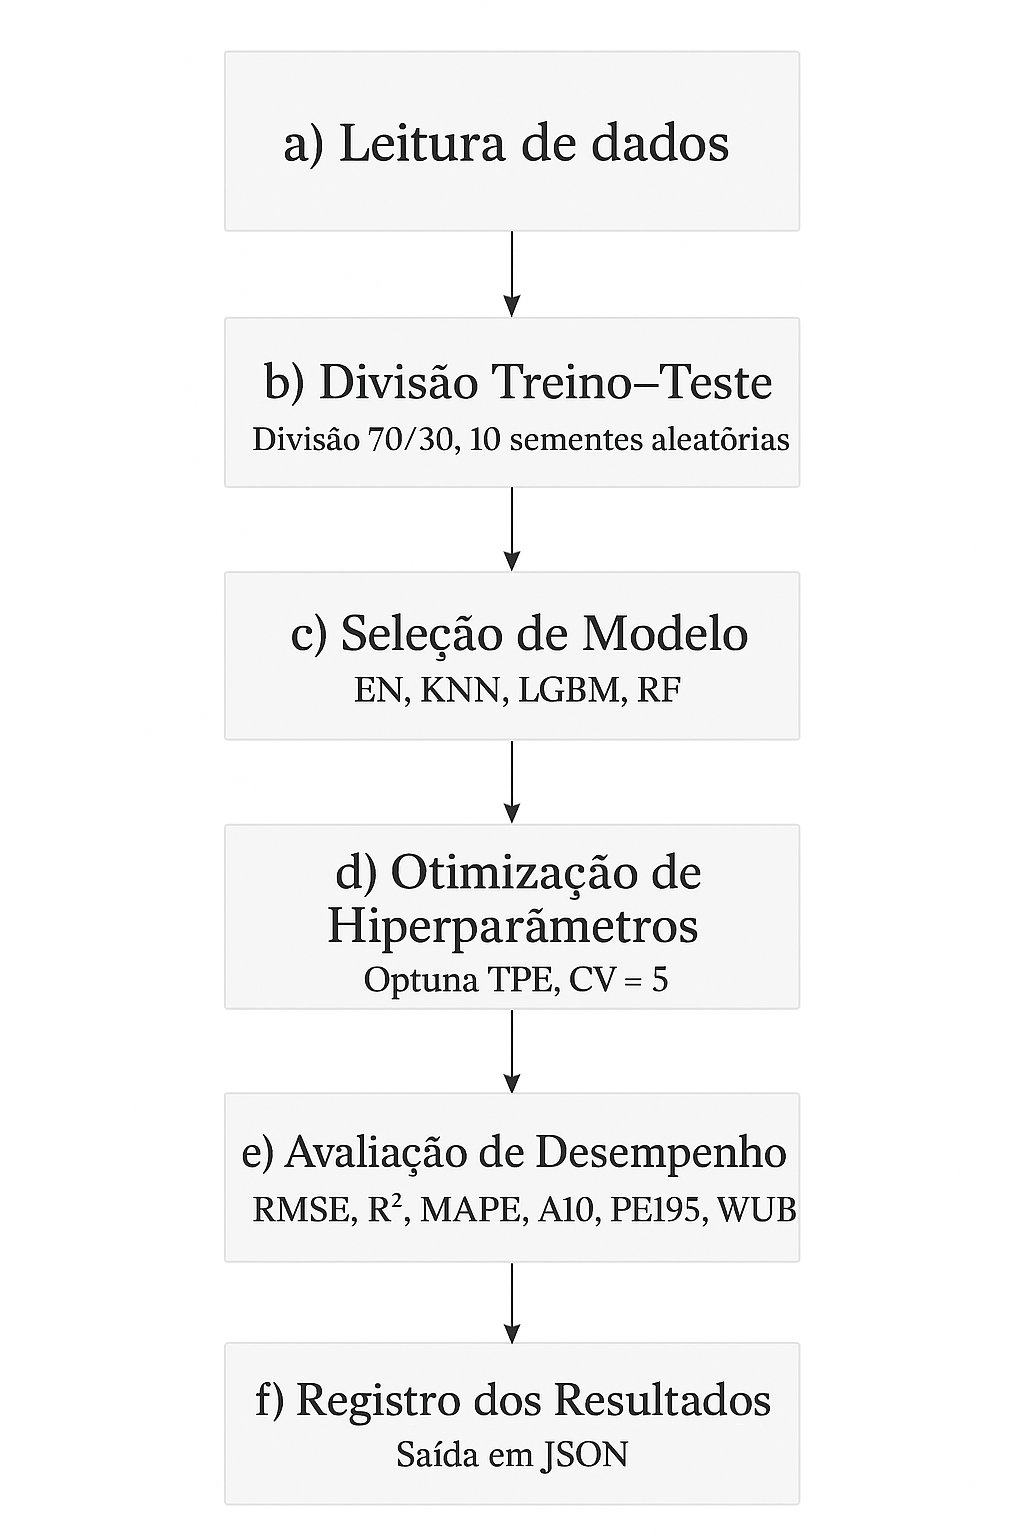
\includegraphics[width=0.5\linewidth]{estrutura_modular.png}
    \fonte{Autor (2025).}
\end{figure}

\begin{alineas}
\item Leitura dos Dados: Os dados estruturados foram importados de um arquivo Excel, considerando o tempo (em segundos) como variável alvo e as demais colunas como preditoras. 
\item Divisão em Conjuntos de Treinamento e Teste: O conjunto de dados foi dividido aleatoriamente em 70\% para treinamento e 30\% para teste, repetindo-se o processo em 10 execuções distintas com sementes aleatórias fixas para garantir robustez nas estimativas. 
\item Seleção dos Modelos: Foram considerados quatro modelos base — \textit{Elastic Net} (EN),\textit{ k-Nearest Neighbors} (KNN), \textit{LightGBM} (LGBM) e \textit{Random Forest} (RF). 
\item Otimização de Hiperparâmetros: O otimizador TPE (\textit{Tree-structured Parzen Estimator}), da biblioteca \textit{Optuna}, foi utilizado para minimizar o erro quadrático médio (MSE) por meio de validação cruzada com cinco subconjuntos (\textit{5-fold cross-validation}), realizando o ajuste tanto dos hiperparâmetros quanto, opcionalmente, das variáveis preditoras. 
\item Avaliação de Desempenho: Os modelos foram avaliados com base nas métricas RMSE, R², MAPE, A10, além de métricas de incerteza como MPE, PEI95 e WUB no conjunto de teste. 
\item Registro dos Resultados: Todas as configurações, previsões e métricas foram armazenadas em formato JSON, garantindo reprodutibilidade e facilitando análises posteriores. 
\end{alineas}

O desempenho dos modelos foi avaliado utilizando cinco métricas padrão no conjunto de teste separado (\textit{hold-out}): erro quadrático médio (RMSE), coeficiente de determinação (R²), coeficiente de correlação de Pearson (R), erro percentual absoluto médio (MAPE) e acurácia dentro de 10\% de desvio (A10).

Com o intuito de garantir a robustez dos resultados, toda a pipeline foi executada em dez rodadas independentes, com diferentes sementes aleatórias. As métricas finais foram reportadas na forma de média ± desvio padrão para cada tipo de modelo avaliado.

As métricas de desempenho agregadas, obtidas a partir de 10 execuções independentes de cada configuração de modelo, utilizando diferentes sementes aleatórias para garantir a robustez, são apresentadas na Tabela \ref{tab:metricas_modelo}. São mostrados a média e o desvio padrão para cinco métricas-chave de avaliação: erro quadrático médio (RMSE), coeficiente de determinação (R²) e acurácia dentro de 10\% de desvio (A10).

% \begin{quadro}[H]
% \centering
% \caption{Métricas do modelo.}
% \label{qua:metricas_modelo}
% \begin{tabular}{|c|c|c|c|c|}
% \hline
% \textbf{Modelo} & \textbf{RMSE} & \textbf{$R^2$} & \textbf{MAPE} & \textbf{A10} \\ \hline
% EN   & 7.365 (0.143) & 0.499 (0.017) & 0.090 (0.002) & 0.729 (0.006) \\ \hline
% KNN  & 2.104 (0.106) & 0.959 (0.004) & 0.024 (0.001) & 0.987 (0.004) \\ \hline
% LGBM & 1.053 (0.091) & 0.990 (0.002) & 0.011 (0.000) & 0.998 (0.002) \\ \hline
% RF   & 1.085 (0.053) & 0.989 (0.001) & 0.012 (0.000) & 0.999 (0.001) \\ \hline
% \end{tabular}
% \fonte{Autor (2025).}
% \end{quadro}

\begin{table}[H]
\centering
\caption{Métricas de desempenho dos modelos de aprendizado.}
\label{tab:metricas_modelo}
\begin{tabularx}{\textwidth}{l *{4}{>{\centering\arraybackslash}X}}
\toprule
\textbf{Modelo} & \textbf{RMSE} & \textbf{$R^2$} & \textbf{MAPE} & \textbf{A10} \\ 
\midrule
Elastic Net (EN) & 7.365 (0.143) & 0.499 (0.017) & 0.090 (0.002) & 0.729 (0.006) \\[3pt]
k-Nearest Neighbors (KNN) & 2.104 (0.106) & 0.959 (0.004) & 0.024 (0.001) & 0.987 (0.004) \\[3pt]
LightGBM (LGBM) & 1.053 (0.091) & 0.990 (0.002) & 0.011 (0.000) & 0.998 (0.002) \\[3pt]
Random Forest (RF) & 1.085 (0.053) & 0.989 (0.001) & 0.012 (0.000) & 0.999 (0.001) \\
\bottomrule
\end{tabularx}
\vspace{0.2cm}
\fonte{Autor (2025).}
\end{table}


Entre os modelos avaliados, o \textit{LightGBM} (LGBM) apresentou, de forma consistente, o melhor desempenho na maioria das métricas, alcançando os menores valores de RMSE e os maiores valores de R². Esse resultado era esperado, dado o potencial do LGBM em capturar padrões complexos e interações não lineares por meio de árvores de decisão com reforço de gradiente. O \textit{Random Forest} (RF) também obteve desempenho satisfatório, com baixa variabilidade entre as execuções, o que evidencia sua estabilidade e robustez frente a ruídos. Em contrapartida, os modelos \textit{Elastic Net} (EN) e \textit{k-Nearest Neighbors} (KNN) apresentaram, em geral, valores mais elevados de RMSE e menores de R². O desempenho inferior do EN pode ser atribuído à sua natureza linear, que limita sua capacidade de modelar relações não lineares presentes nos dados. Já o KNN demonstrou maior variabilidade, possivelmente devido à sua sensibilidade à estrutura local dos dados e à escala das variáveis. A Figura \ref{fig:result_modelos} mostra, graficamente, os resultados obtidos.

\begin{figure}[H]
\centering
\caption{Valores observados versus previstos para cada modelo.}
\label{fig:result_modelos}
\begin{subfigure}[t]{0.45\textwidth}
    \centering
    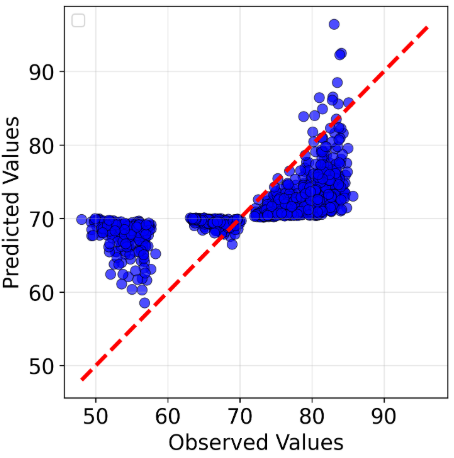
\includegraphics[width=\linewidth]{z_po_en.png}
    \caption{EN}
\end{subfigure}
\hspace{0.2cm}
\begin{subfigure}[t]{0.45\textwidth}
    \centering
    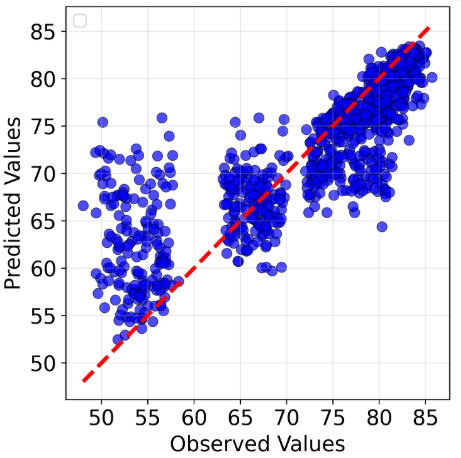
\includegraphics[width=\linewidth]{z_po_knn.png}
    \caption{KNN}
\end{subfigure}

\vspace{0.2cm}

\begin{subfigure}[t]{0.45\textwidth}
    \centering
    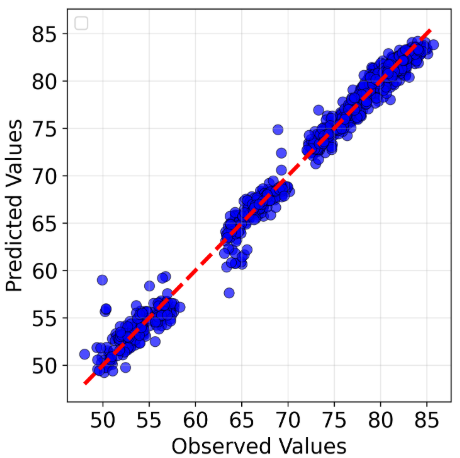
\includegraphics[width=\linewidth]{z_po_lgbm.png}
    \caption{LGBM}
\end{subfigure}
\hspace{0.2cm}
\begin{subfigure}[t]{0.45\textwidth}
    \centering
    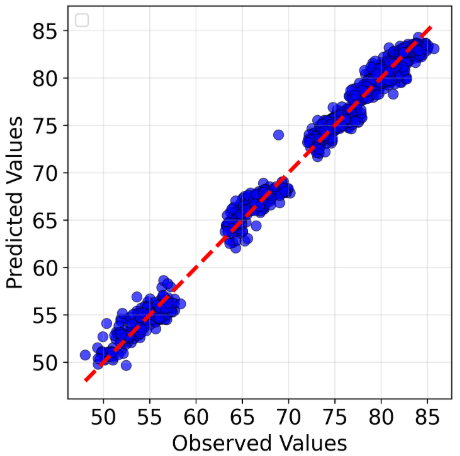
\includegraphics[width=\linewidth]{z_po_rf.png}
    \caption{RF}
\end{subfigure}
\vspace{0.2cm}
\fonte{Autor (2025).}
\end{figure}

% A variação no desempenho entre os modelos e diferentes sementes reforça a importância da seleção adequada do modelo e da calibração dos hiperparâmetros em problemas de engenharia orientados por dados. Esses resultados justificam a adoção da abordagem por comitê (\textit{ensemble}) utilizada neste estudo, que combina as forças de cada modelo individual, ao mesmo tempo em que mitiga suas limitações por meio da agregação ponderada. Cada subgráfico exibe a relação entre os valores previstos pelo modelo e os valores reais obtidos, permitindo avaliar visualmente a precisão de cada método. A linha diagonal indica a condição ideal de predição, na qual os valores estimados coincidem perfeitamente com os observados. Quanto mais próximos os pontos estiverem dessa linha, melhor o desempenho do modelo.

% Observa-se que o modelo Random Forest apresenta maior concentração de pontos próximo da linha de referência quando comparado aos demais algoritmos, indicando melhor capacidade preditiva e menor dispersão dos erros. O LGBM também apresenta boa performance, embora com dispersão ligeiramente superior. Já os modelos Elastic Net e KNN demonstram maior variabilidade nas previsões, sobretudo em regiões mais afastadas da diagonal, revelando limitações no ajuste às características dos dados deste estudo. Assim, com base na análise visual e quantitativa dos resultados, o modelo Random Forest mostrou-se a alternativa mais eficiente para o problema em questão, sendo selecionado como método final para a estimativa da vida útil remanescente das estruturas avaliadas.

% A Figura \ref{fig:media_impor} compara a média da importância das variáveis com base na técnica de \textit{permutation feature importance} para os modelos EN, KNN, LGBM e RF. Em todos os casos, as variáveis de carregamento $m_{gk}$ e $m_{qk}$ demonstraram maior relevância, evidenciando sua influência predominante sobre o tempo de simulação. Os modelos LGBM e RF, por serem baseados em árvores, capturam essas dependências não lineares com maior clareza, enquanto o EN, por sua linearidade, apresenta uma importância mais distribuída, porém menos expressiva. O modelo KNN também destacou variáveis relacionadas a carregamento, reflexo de sua dependência de métricas de distância. Já as variáveis geométricas ($b_w$, $h$) e de material ($f_{ck}$) apresentaram menor relevância, sugerindo que a magnitude das cargas é o principal fator determinante da complexidade computacional das simulações.

% \begin{figure}[H]
%     \centering
%     \caption{Média da importância das variáveis.}
%     \label{fig:media_impor}
%     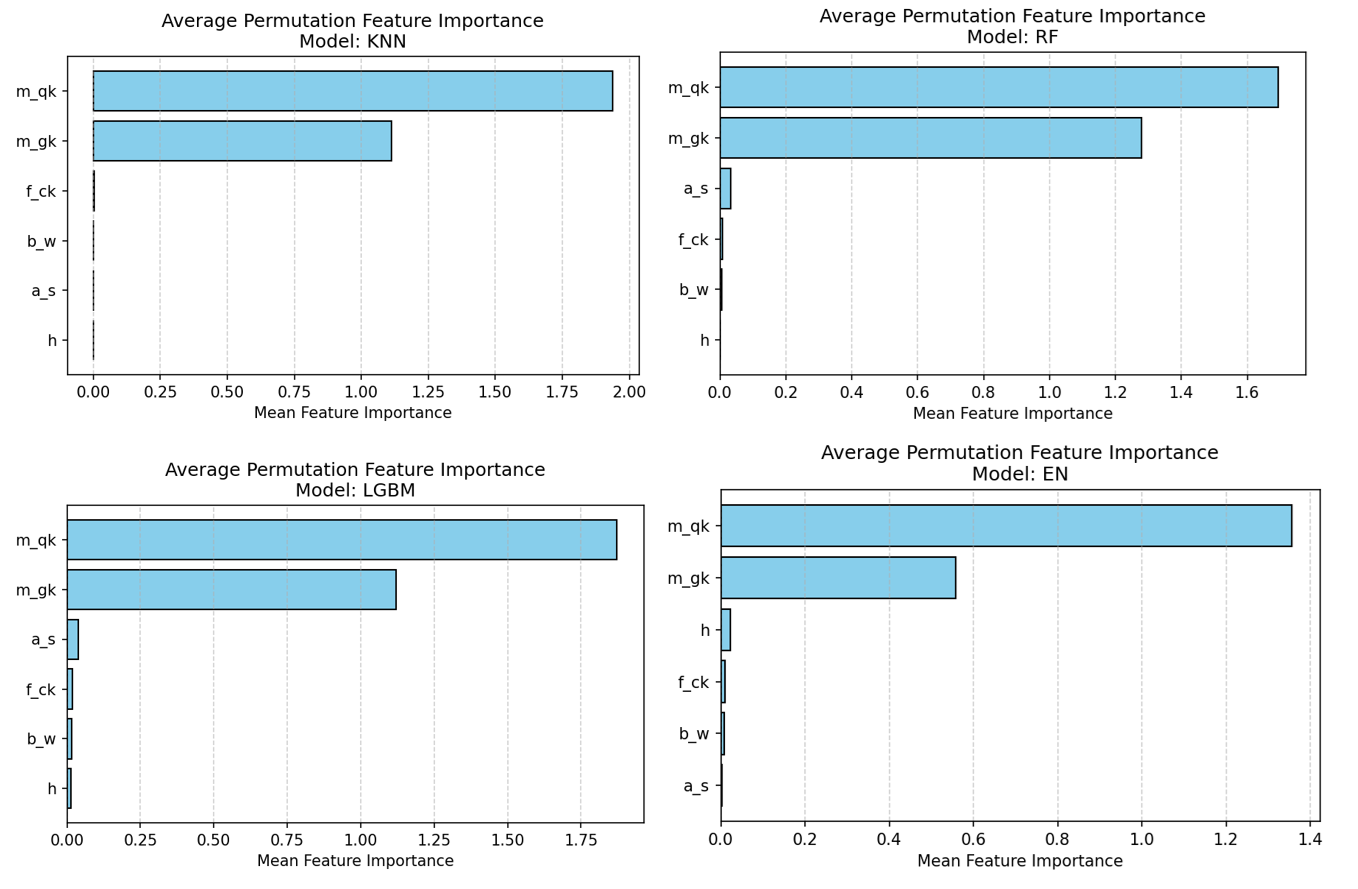
\includegraphics[width=\linewidth]{average permutation feature importance.png}
%     \fonte{Autor (2025).}
% \end{figure}

% A Tabela \ref{tab:metricas} apresenta as métricas de incerteza para cada modelo, medidas por meio da largura das bandas de incerteza (\textit{Width of Uncertainty Bands} – WUB) e do intervalo de predição com 95\% de confiança (\textit{Prediction Error Interval} 95\% – PEI95). Como era esperado, os modelos baseados em comitê, LGBM e RF, apresentaram os menores valores de incerteza, com WUB variando entre 1,05 e 1,08 e PEI95 entre 4,1 e 4,3. Esses resultados refletem a elevada capacidade de generalização e a robustez desses modelos frente a diferentes configurações de dados.

% % \begin{quadro}[H]
% % \centering
% % \caption{Métricas de incerteza (WUB e PEI95) para cada modelo. Os valores entre parênteses correspondem ao desvio padrão.}
% % \label{qua:Qua_5}
% % \begin{tabular}{|c|c|c|}
% % \hline
% % \textbf{Modelo} & \textbf{WUB} & \textbf{PEI95} \\ \hline
% % KNN  & 2.104 (0.101) & 8.249 (0.395) \\ \hline
% % LGBM & 1.053 (0.086) & 4.128 (0.339) \\ \hline
% % RF   & 1.085 (0.050) & 4.254 (0.195) \\ \hline
% % EN   & 7.364 (0.137) & 28.869 (0.537) \\ \hline
% % \end{tabular}
% % \fonte{Autor (2025).}
% % \end{quadro}

% \begin{table}[H]
% \centering
% \caption{Métricas de incerteza (WUB e PEI95) para cada modelo.}
% \label{tab:metricas}
% \begin{tabular}{p{4cm} p{5cm} p{5cm}}
% \toprule
% \textbf{Modelo} & \textbf{WUB} & \textbf{PEI95} \\ 
% \midrule
% KNN  & 2.104 (0.101) & 8.249 (0.395) \\ 
% LGBM & 1.053 (0.086) & 4.128 (0.339) \\ 
% RF   & 1.085 (0.050) & 4.254 (0.195) \\ 
% EN   & 7.364 (0.137) & 28.869 (0.537) \\ 
% \bottomrule
% \end{tabular}
% \fonte{Autor (2025).}
% \end{table}

% Em síntese, os resultados demonstram que os modelos baseados em árvores de decisão, \textit{LightGBM} e \textit{Random Forest}, apresentaram desempenho superior na previsão do tempo de simulação, alcançando menor erro, maior precisão e menor incerteza em comparação aos modelos lineares (\textit{Elastic Net}) e não paramétricos (\textit{KNN}). A análise de importância das variáveis evidenciou que os carregamentos aplicados às vigas são os fatores determinantes para a complexidade computacional, enquanto características geométricas e de material têm menor influência. Esses achados confirmam a relevância de adotar métodos de aprendizado de máquina e técnicas de ensemble para capturar padrões complexos e não lineares, fornecendo uma ferramenta robusta e escalável para avaliação da confiabilidade estrutural de estruturas de concreto armado. Além disso, a quantificação da incerteza por meio de métricas como PEI95 e WUB reforça a capacidade dos modelos de oferecer previsões confiáveis, alinhando-se diretamente aos objetivos do estudo de fornecer suporte à tomada de decisão em manutenção e gestão de estruturas sujeitas à corrosão.

% Dessa forma, foi selecionado o método \textit{Random Forest} para a geração do modelo preditivo. A Figura \ref{fig:random_forest} ilustra o princípio de funcionamento desse algoritmo, que se baseia na construção e combinação de múltiplas árvores de decisão de forma independente.

% \begin{figure}[H]
% \centering
% \caption{Representação do método \textit{Random Forest}.}
% \label{fig:random_forest}
% 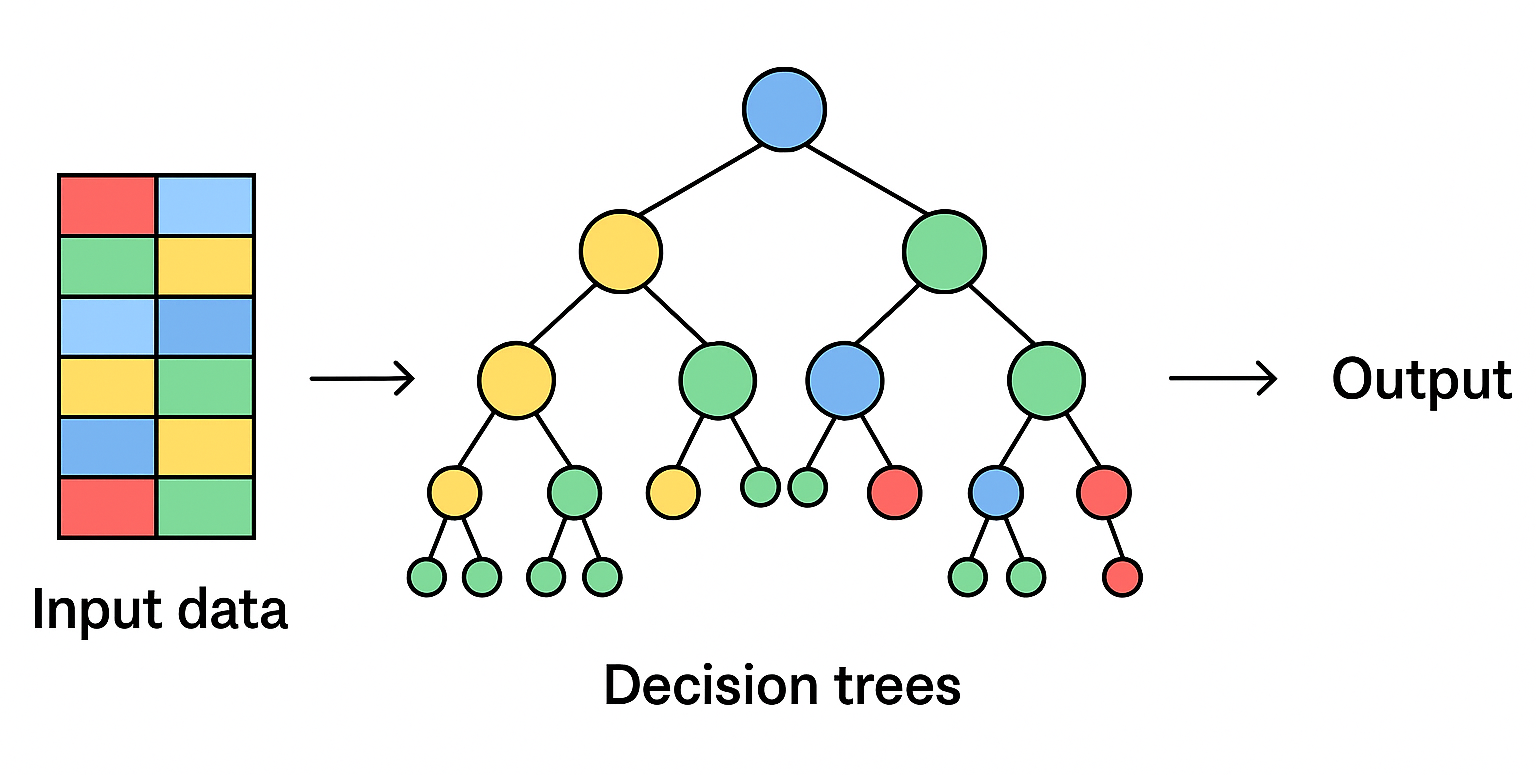
\includegraphics[width=0.7\linewidth]{random_forest.png}
% \fonte{Autor (2025).}
% \end{figure}

% Na Figura \ref{fig:random_forest}, observa-se, à esquerda, o conjunto de dados de entrada, composto por diferentes variáveis utilizadas no treinamento do modelo. Esses dados alimentam várias árvores de decisão independentes, representadas no centro da figura. Cada árvore é construída a partir de subconjuntos aleatórios de amostras e de variáveis, promovendo diversidade e reduzindo a correlação entre os classificadores individuais.

% Por fim, à direita, o resultado final é obtido pela combinação das previsões de todas as árvores, geralmente por votação majoritária, no caso de problemas de classificação, ou pela média das estimativas, no caso de regressão. Essa abordagem permite que o \textit{Random Forest} produza uma previsão mais estável, precisa e menos sensível a ruídos ou a outliers, quando comparado a modelos baseados em uma única árvore de decisão.


\section{Determinação da Vida Útil Remanescente (VUR)} \label{sec:res_vur}

Na avaliação da vida útil remanescente das estruturas, foi desenvolvido um modelo capaz de extrair três estatísticas fundamentais do sistema, conforme descrito a seguir:

\begin{enumerate}[label=(\alph*)]
    \item Tempo de vida útil da estrutura: definido como o instante em que a função de estado limite assume valor inferior a zero, indicando a ocorrência da falha estrutural;
    
    \item Valor da função de estado limite em um tempo genérico $t_i$: para um instante qualquer $t_i$, a função de estado limite $g(\textbf{R}, \textbf{S}, t_i)$ é avaliada, possibilitando o acompanhamento da degradação da capacidade resistente ao longo do tempo;
    
    \item Tempo de vida útil condicional: considerando um instante $t_i$ arbitrário, é determinado o tempo necessário para que uma amostra $k$ atinja o valor de $g = 0$ a partir desse instante. Essa estatística permite estimar a vida útil residual da estrutura, a partir de um estado de deterioração intermediário.
\end{enumerate}

Esse procedimento fornece a base necessária para análises de confiabilidade dependentes do tempo, permitindo identificar o instante de falha estrutural e descrever o comportamento probabilístico da degradação ao longo da vida útil de projeto. A partir dessas estatísticas, busca-se desenvolver um modelo preditivo capaz de estimar, com maior precisão, a vida útil remanescente de vigas de concreto armado com armadura simples, considerando a evolução progressiva dos mecanismos de deterioração.

Como etapa complementar à avaliação da vida útil estrutural, foram elaboradas distribuições empíricas na forma de histogramas, construídos a partir do banco de dados gerado pelo modelo probabilístico. Os histogramas organizam as amostras em intervalos (\textit{bins}), permitindo observar a distribuição de frequência das variáveis de interesse e evidenciar padrões relevantes, tais como dispersão, assimetria e tendência central, contribuindo para uma interpretação mais robusta dos resultados obtidos.

Na Figura \ref{fig:histogramas} apresentam-se três histogramas correspondentes aos resultados do estudo para um tempo de análise $t_i = 35$ anos:

\begin{figure}[H]
    \centering
    \caption{Histogramas.}
    \label{fig:histogramas}
    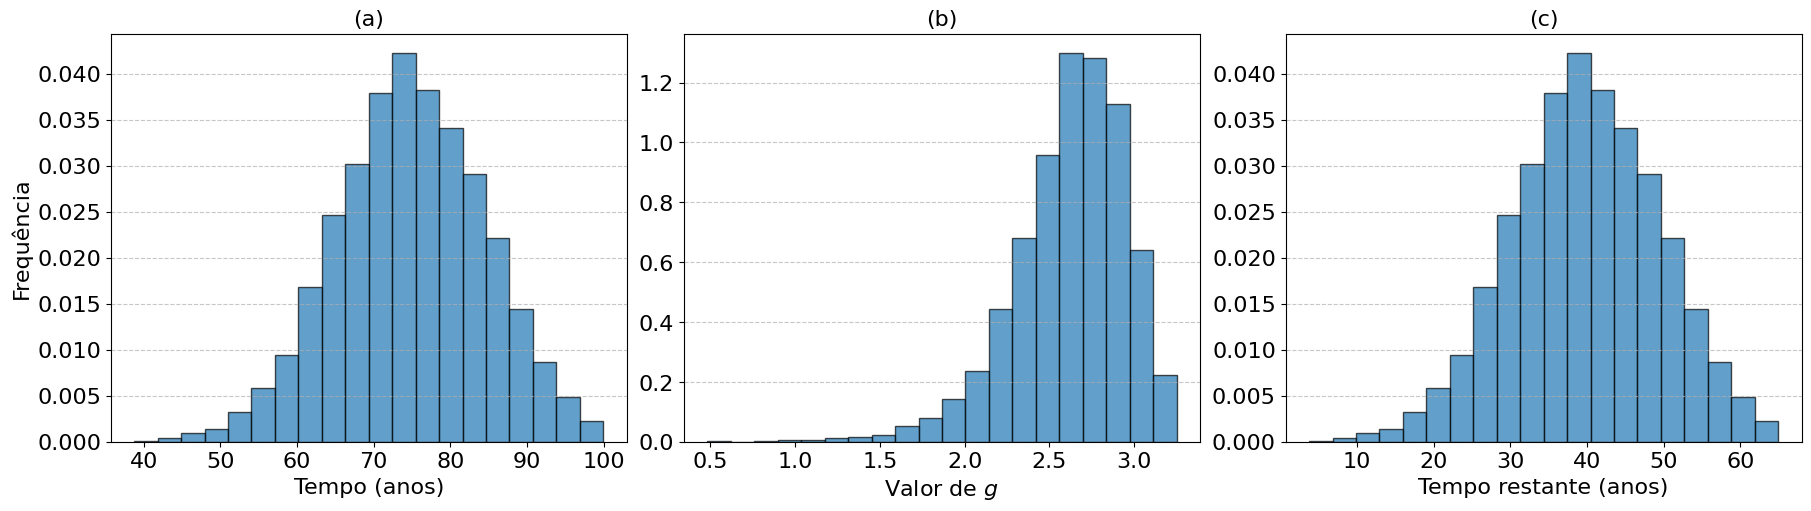
\includegraphics[width=\linewidth]{histogramas.png}
    \fonte{Autor (2025).}
\end{figure}

\begin{itemize}
    \item Histograma (a) – Tempo de vida útil total: mostra a distribuição dos tempos em que a função de estado limite \(g(t)\) cruza o valor zero, indicando a falha estrutural completa das vigas. Este histograma permite observar a variabilidade do tempo de vida útil prevista pelo modelo probabilístico.
    
    \item Histograma (b) – Valor da função de estado limite em $t_i$: apresenta a distribuição dos valores de \(g(t_i)\) no instante escolhido de 35 anos. Este gráfico evidencia o nível de segurança residual da estrutura naquele instante, permitindo avaliar a proximidade da falha.
    
    \item Histograma (c) – Vida útil residual após $t_i$: ilustra a distribuição do tempo restante para que cada amostra alcance \(g = 0\), a partir do instante $t_i = 35$ anos. Este histograma fornece informações sobre a vida útil remanescente das vigas condicionada ao estado atual de deterioração.
\end{itemize}

Em síntese, o modelo desenvolvido viabilizou a extração de estatísticas essenciais para a caracterização da vida útil de vigas de concreto armado, incluindo o tempo total até a falha, a evolução da função de estado limite ao longo do tempo e a vida útil remanescente condicionada a diferentes estados de deterioração. A análise dos histogramas revelou a variabilidade intrínseca ao comportamento estrutural e permitiu identificar tendências e padrões de degradação progressiva.

Os resultados obtidos fornecem uma base consistente para avaliações probabilísticas de confiabilidade estrutural dependente do tempo, possibilitando estimativas fundamentadas da Vida Útil Remanescente (VUR). Além disso, esses achados sustentam o desenvolvimento de modelos preditivos robustos e escaláveis, alinhados ao propósito deste estudo de disponibilizar ferramentas assertivas para o planejamento de manutenção e a gestão do ciclo de vida de estruturas sujeitas à corrosão.

\section{Verificação do Emulador Estocástico em Problema de Referência} \label{sec:res_emulador}

Os resultados apresentados nas seções anteriores demonstram que modelos de regressão supervisionada reproduzem com boa acurácia o tempo de vida útil obtido por simulação de Monte Carlo. Essa abordagem, contudo, fornece uma predição \textit{pontual}: para cada configuração de viga, obtém-se um único valor de tempo de vida útil, e a informação sobre a dispersão em torno dessa estimativa precisa ser recuperada indiretamente, por meio de métricas de incerteza do próprio regressor. A frente de trabalho descrita nesta seção busca superar essa limitação, emulando a \textit{distribuição condicional completa} da função de estado limite ao longo do tempo, conforme a formulação apresentada na \autoref{sec:construcao_emulador}.

Antes de aplicar o emulador ao problema da viga sob carbonatação, cuja resposta não possui solução analítica de referência, verificou-se o arcabouço metodológico em um problema de referência de baixo custo computacional, no qual a solução por simulação direta de Monte Carlo pode ser obtida e utilizada como valor de referência (\textit{ground truth}). Essa estratégia de verificação segue a prática recomendada por \textcite{pires2024}. Cabe registrar que as figuras desta seção foram geradas na etapa de verificação do método e mantêm os rótulos em língua inglesa, que serão traduzidos na versão final do texto.

\subsection{Definição do Problema de Referência}

Adota-se uma versão adaptada de um problema clássico de confiabilidade, definida pela Equação \eqref{eq:toy_problem_equation}. Nessa formulação, $\mathbf{R}$ e $\mathbf{S}$ denotam, respectivamente, a resistência estrutural e a solicitação. A dependência temporal é introduzida por um fator de degradação linear aplicado à resistência, $k_{fator}(t)$, que modela a redução progressiva da capacidade ao longo da vida útil, com $k_{inicial} = 1{,}0$ no instante inicial e $k_{final} = 0{,}3$ ao final do horizonte $T_f = 100$ anos, conforme a Equação \eqref{eq:k_factor_linear}. As incertezas de modelagem são incorporadas pelas variáveis latentes $\mathbf{Z}_1$ e $\mathbf{Z}_2$, que afetam, respectivamente, a resistência e a solicitação --- exatamente o papel desempenhado pelos erros de modelo $E_r$ e $E_s$ na função de estado limite do problema da viga, Equação \eqref{eq:estado_limite}.

\begin{equation}\label{eq:k_factor_linear}
k_{fator}(t) =
\begin{cases}
k_{inicial}, & t \leq 0 \\[5pt]
k_{final}, & t \geq T_f \\[5pt]
k_{inicial} + (k_{final} - k_{inicial}) \cdot \dfrac{t}{T_f}, & 0 < t < T_f
\end{cases}
\end{equation}

\begin{equation}\label{eq:toy_problem_equation}
g(\mathbf{R}, \mathbf{S}, t) = k_{fator}(t) \cdot \frac{\mathbf{R}}{\mathbf{Z}_1} - \mathbf{S} \cdot \mathbf{Z}_2
\end{equation}

Os parâmetros estatísticos das variáveis aleatórias do problema de referência são apresentados na Tabela \ref{tab:random_variables_parameters}.

\begin{table}[H]
\centering
\caption{Parâmetros estatísticos e distribuições das variáveis do problema de referência.}
\label{tab:random_variables_parameters}
\begin{tabular}{l c c c c}
\toprule
\textbf{Variável} & \textbf{Símbolo} & \textbf{Distribuição} & \textbf{Média} & \textbf{Desvio padrão} \\
\midrule
Resistência                       & $R$   & Normal    & 5,00 & 0,80  \\
Solicitação                       & $S$   & Normal    & 2,00 & 0,60  \\
Incerteza de modelo (resistência) & $Z_1$ & Lognormal & 1,00 & 0,028 \\
Incerteza de modelo (solicitação) & $Z_2$ & Lognormal & 1,00 & 0,096 \\
\bottomrule
\end{tabular}
\vspace{0.2cm}
\fonte{Autor (2025).}
\end{table}

\subsection{Comportamento Temporal dos Parâmetros da GLD}

A análise dependente do tempo considerou 10 passos igualmente espaçados em um horizonte de 100 anos. Em cada passo, realizações da função de estado limite foram avaliadas e os quatro parâmetros da GLD, $\lambda_1$ a $\lambda_4$, foram ajustados via PyGLAM. Para fins ilustrativos, adotaram-se as realizações fixas $r = 5{,}09$ e $s = 1{,}80$, com 2.000 amostras das variáveis latentes por passo de tempo. A Figura \ref{fig:g_function_realizations} mostra a evolução temporal da função de estado limite, refletindo claramente a influência do fator de degradação, e a correspondente evolução dos parâmetros da GLD.

\begin{figure}[H]
    \centering
    \caption{Avaliação da função $g$ ao longo do tempo.}
    \label{fig:g_function_realizations}
    \begin{subfigure}{0.9\textwidth}
        \centering
        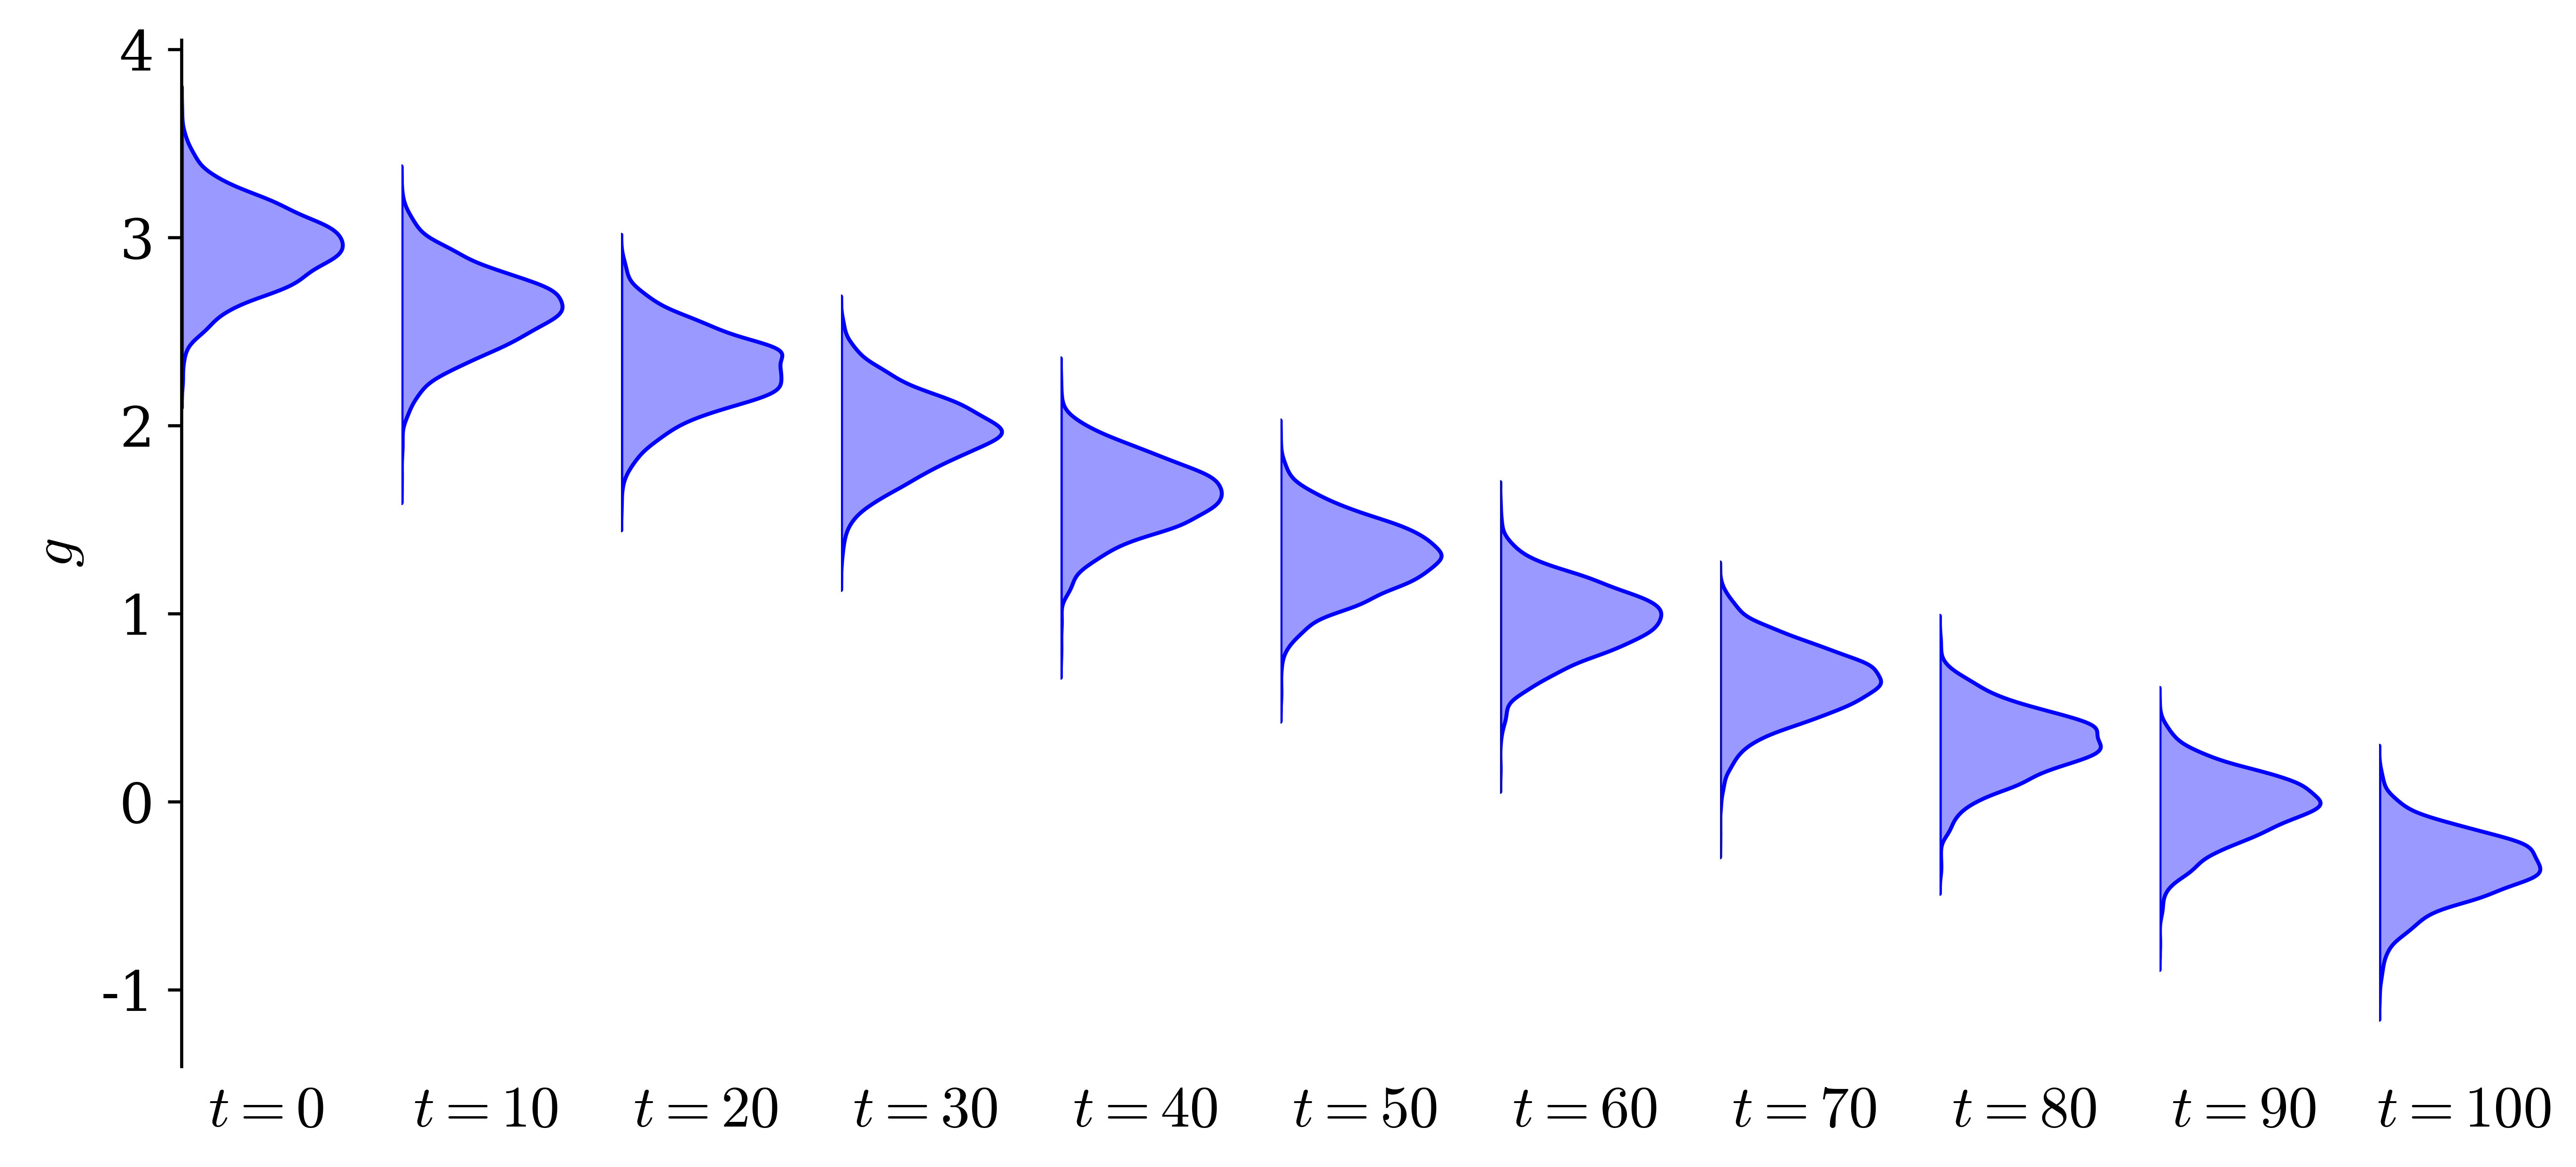
\includegraphics[width=\textwidth]{z_time-lapse_g_analysis_en.png}
        \caption{Realizações com valores fixos $r = 5{,}09$ e $s = 1{,}80$.}
        \label{fig:g_realizacoes}
    \end{subfigure}
    \vspace{0.3cm}
    \begin{subfigure}{0.95\textwidth}
        \centering
        
\includegraphics[width=\textwidth]{z_lambdas_for_r_s_realization_en.png}
        \caption{Evolução de $\lambda_1$ a $\lambda_4$ no tempo.}
        \label{fig:lambdas_tempo}
    \end{subfigure}
    \vspace{0.2cm}
    \fonte{Autor (2025).}
\end{figure}

Previamente ao treinamento do metamodelo, conduziu-se uma avaliação exploratória da sensibilidade dos parâmetros da GLD: 1.000 realizações de $r$ e $s$, combinadas a 2.000 amostras das variáveis latentes, foram analisadas em $t = 0$ e $t = 50$ anos. Os resultados demonstram que $\lambda_1$ e $\lambda_2$ apresentam sensibilidade pronunciada às variações de $\mathbf{R}$ e $\mathbf{S}$, enquanto $\lambda_3$ e $\lambda_4$ exibem baixa dispersão e fraca dependência das entradas. Com base nessa evidência, apenas $\lambda_1$ e $\lambda_2$ foram selecionados como variáveis-alvo do treinamento, sendo $\lambda_3$ e $\lambda_4$ representados por seus valores médios.

A Tabela \ref{tab:validation_results} confirma essa decisão: os altos valores de $R^2$ obtidos para $\lambda_1$ e $\lambda_2$ em todos os passos de tempo indicam excelente acurácia preditiva da PCE, enquanto os valores consistentemente baixos para $\lambda_3$ e $\lambda_4$ corroboram sua exclusão do treinamento. Observa-se, ainda, uma queda progressiva do $R^2$ dos parâmetros de forma com o avanço do tempo, comportamento coerente com a redução da variabilidade relativa desses parâmetros à medida que a degradação se acentua.

\begin{table}[H]
\centering
\caption{Validação estatística do metamodelo PCE em diferentes passos de tempo (valores de $R^2$).}
\label{tab:validation_results}
\begin{tabular}{rrrrr}
\toprule
\textbf{Tempo (anos)} & $\boldsymbol{\lambda_1}$ & $\boldsymbol{\lambda_2}$ & $\boldsymbol{\lambda_3}$ & $\boldsymbol{\lambda_4}$ \\
\midrule
0   & 1,0000 & 0,9839 & 0,3858 & 0,3978 \\
20  & 1,0000 & 0,9894 & 0,3713 & 0,3804 \\
40  & 1,0000 & 0,9792 & 0,4081 & 0,3891 \\
60  & 1,0000 & 0,9926 & 0,3102 & 0,3525 \\
80  & 1,0000 & 0,9918 & 0,2277 & 0,2146 \\
100 & 1,0000 & 0,9865 & 0,0638 & 0,1352 \\
\bottomrule
\end{tabular}
\vspace{0.2cm}
\fonte{Autor (2025).}
\end{table}

\subsection{Qualidade da Distribuição Emulada}

A Figura \ref{fig:kde_comparison} compara, por estimativa de densidade por núcleo (KDE), a distribuição de referência e a aproximação obtida via emulador PCE--GLD para as realizações fixas $r = 5{,}09$ e $s = 1{,}80$, nos instantes $t = 0$ e $t = 50$ anos.

\begin{figure}[H]
    \centering
    \caption{Comparação entre a distribuição de referência e a aproximação do emulador.}
    \label{fig:kde_comparison}
    \begin{subfigure}[b]{0.42\textwidth}
        \centering
        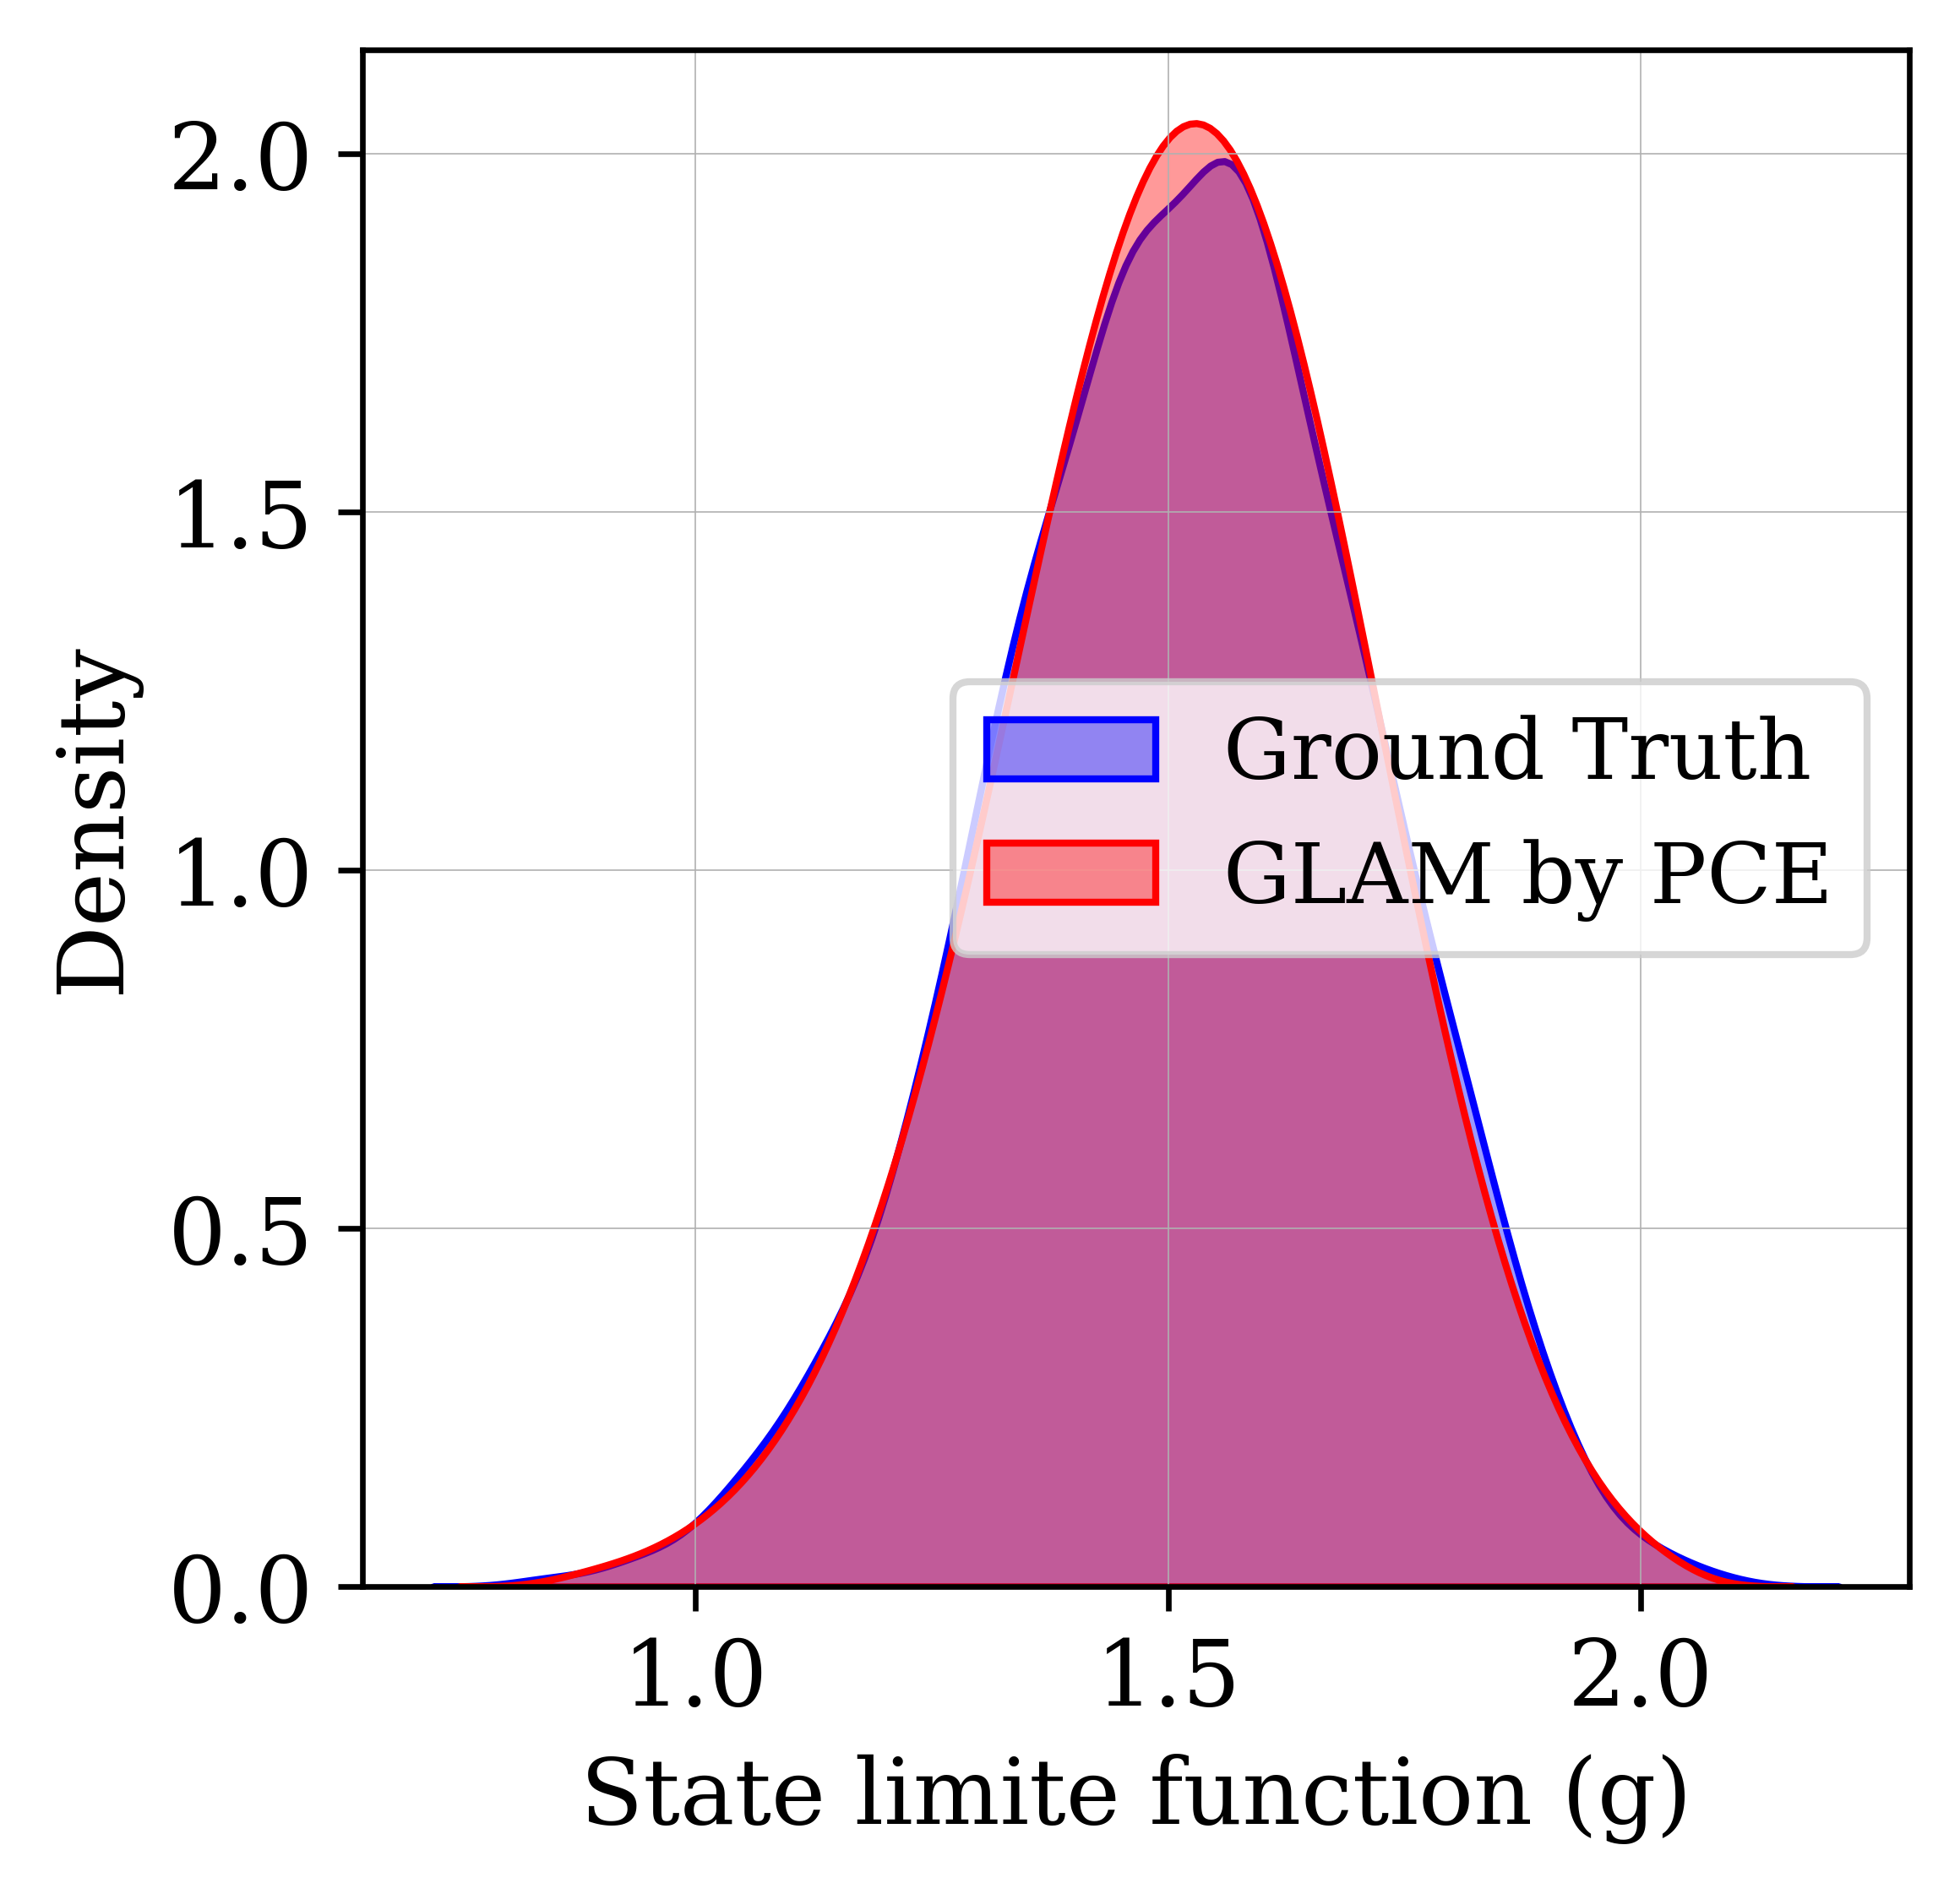
\includegraphics[width=\textwidth]{z_histogram_glam_versus_gt_t0_en.png}
        \caption{$t = 0$}
        \label{fig:kde_t0}
    \end{subfigure}
    \hfill
    \begin{subfigure}[b]{0.42\textwidth}
        \centering
        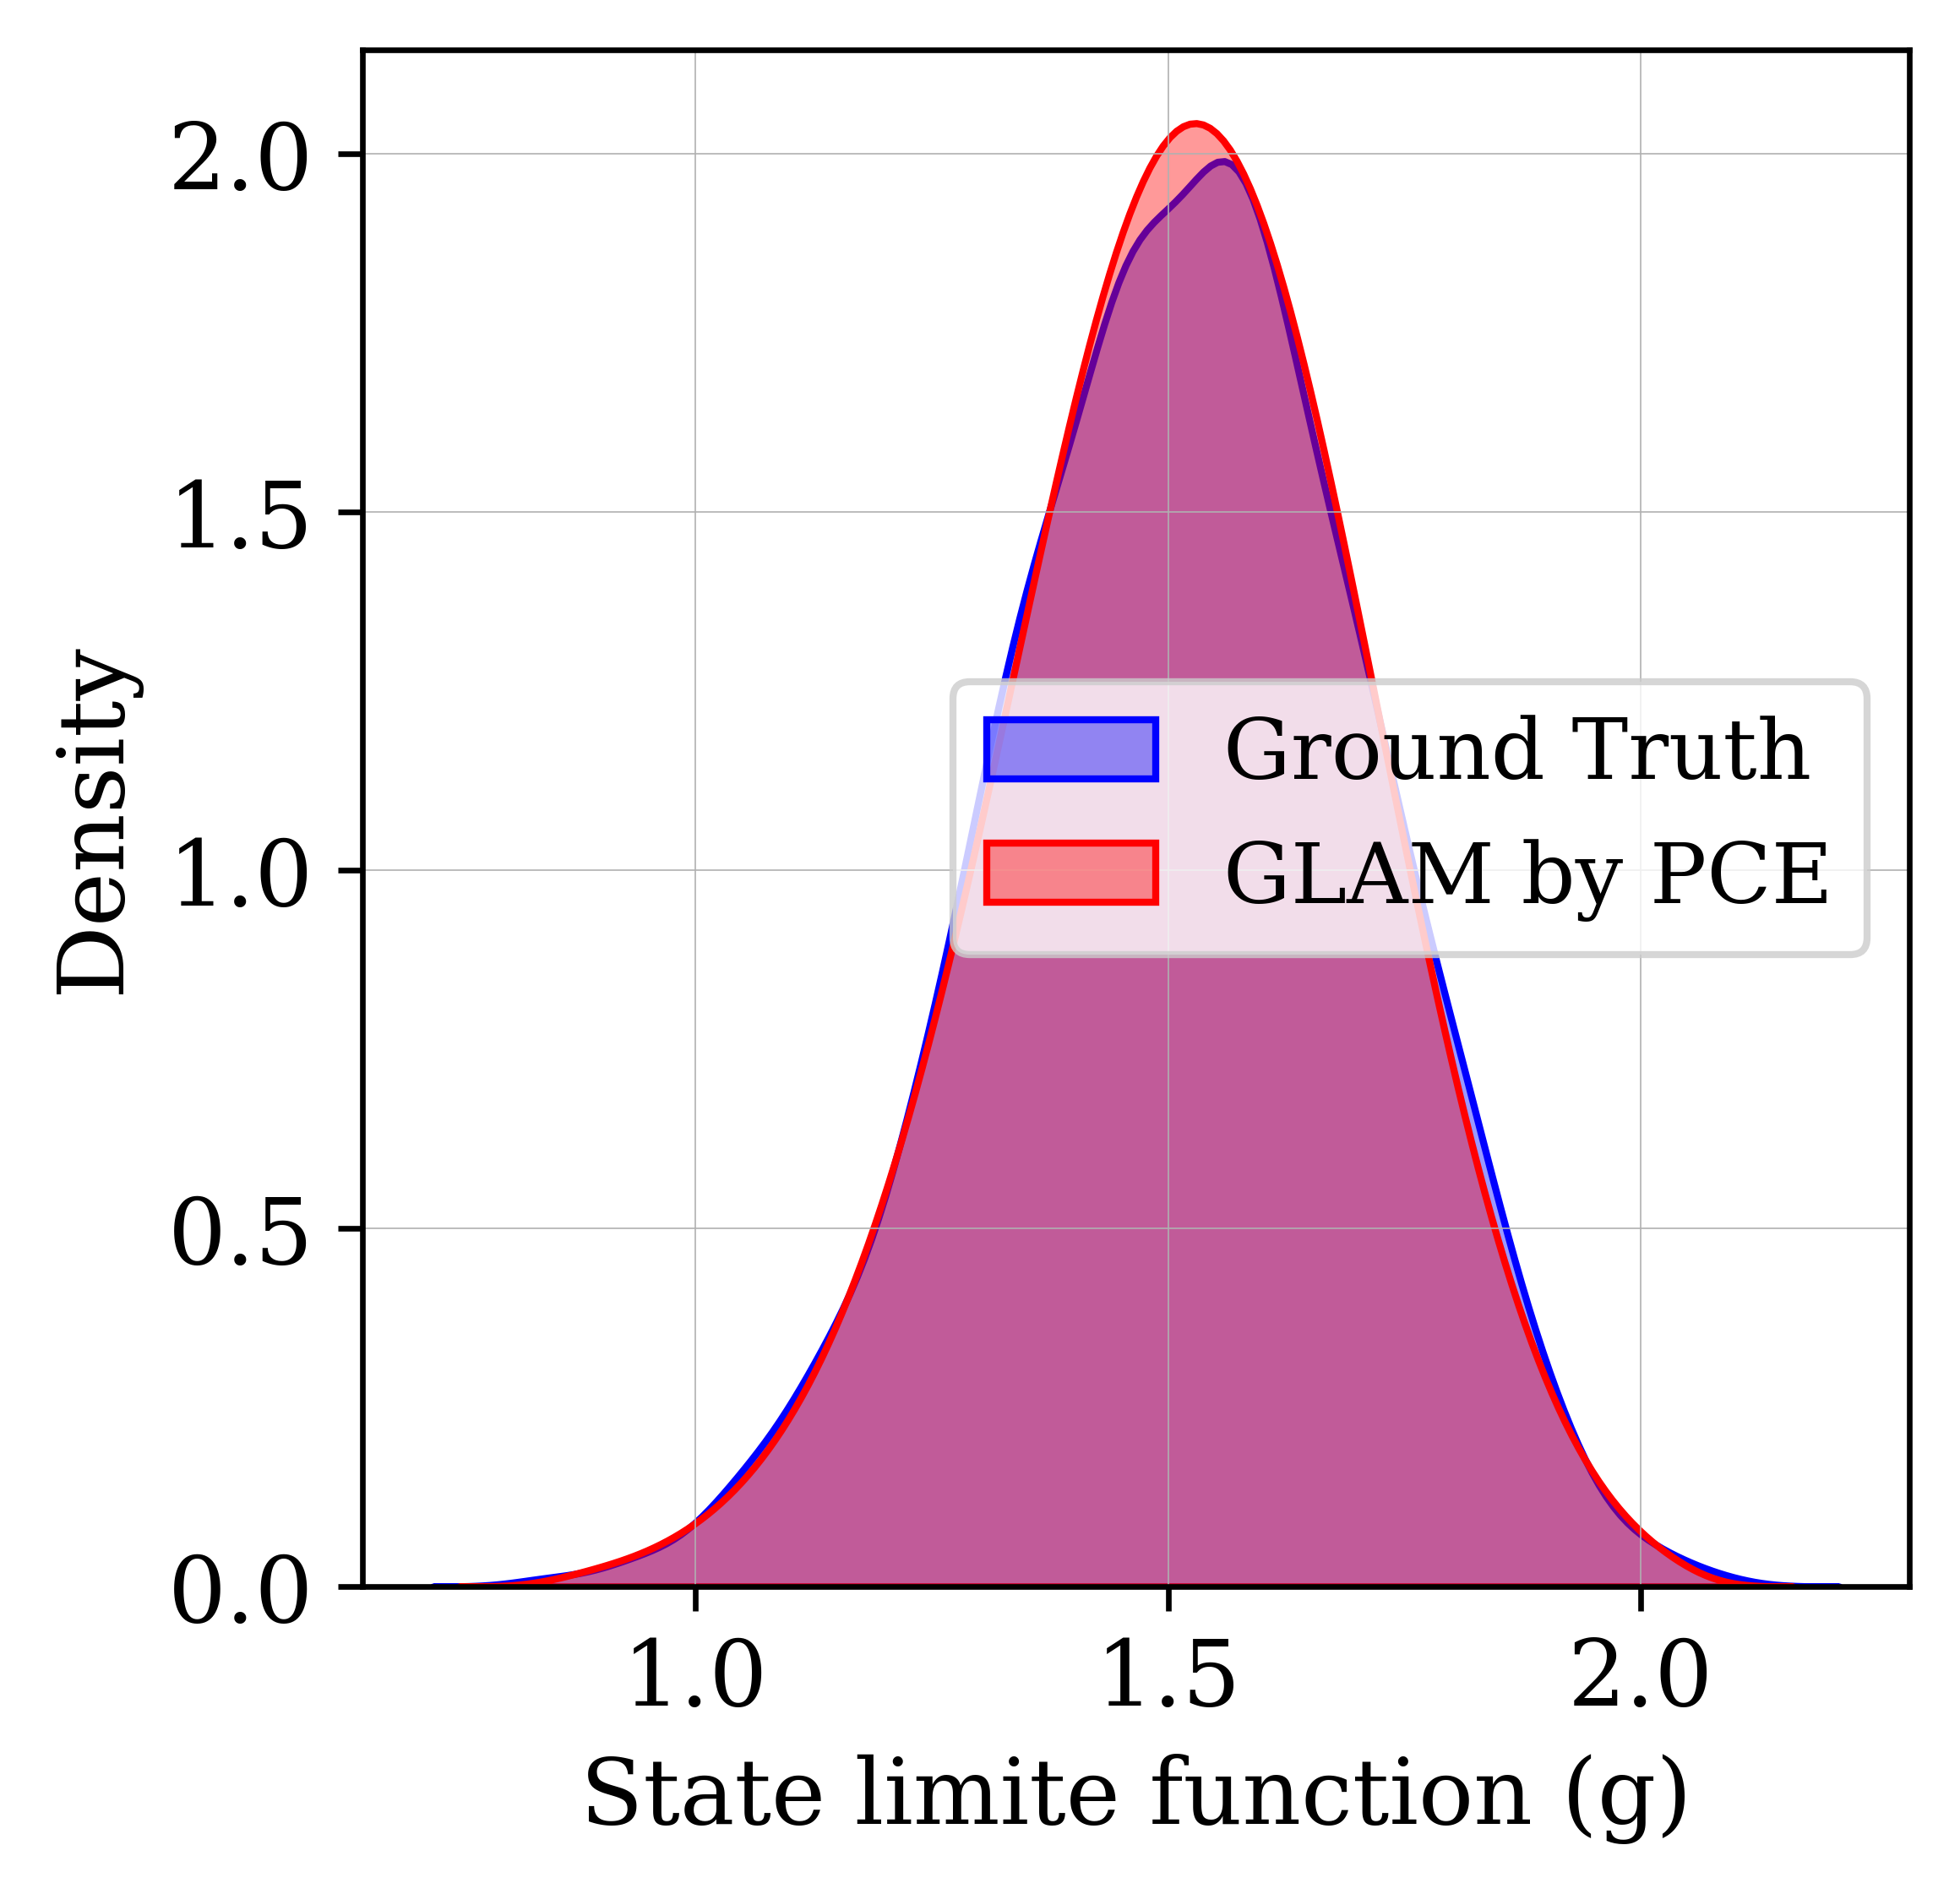
\includegraphics[width=\textwidth]{z_histogram_glam_versus_gt_t50_en.png}
        \caption{$t = 50$ anos}
        \label{fig:kde_t50}
    \end{subfigure}
    \vspace{0.2cm}
    \fonte{Autor (2025).}
\end{figure}

A similaridade estatística foi quantificada pelos testes de aderência e pela comparação de quantis descritos na \autoref{sec:metricas_emulador}, com resultados nas Tabelas \ref{tab:statistical_tests} e \ref{tab:quantile_comparison}. O teste de Kolmogorov--Smirnov não rejeita a hipótese nula ao nível de 5\% ($D = 0{,}0108$; valor-p $= 0{,}9325$), indicando excelente concordância global entre as funções de distribuição empíricas. O teste de Anderson--Darling, em contraste, rejeita a hipótese nula, comportamento atribuído à sua elevada sensibilidade às caudas em amostras grandes \cite{scholz1987}.

\begin{table}[H]
\centering
\caption{Testes de aderência entre a referência e o emulador.}
\label{tab:statistical_tests}
\begin{tabular}{lcccc}
\toprule
\textbf{Teste} & \textbf{Estatística} & \textbf{valor-p} & \textbf{Nível ($\alpha$)} & \textbf{Decisão} \\
\midrule
Kolmogorov--Smirnov & 0,0108      & 0,9325 & 0,05 & Não rejeita $H_0$ \\
Anderson--Darling   & $-0{,}6492$ & 0,0025 & 0,05 & Rejeita $H_0$ \\
\bottomrule
\end{tabular}
\vspace{0.2cm}
\fonte{Autor (2025).}
\end{table}

A análise de quantis localiza a origem dessa discrepância. Conforme a Tabela \ref{tab:quantile_comparison}, os erros relativos permanecem abaixo de 0,5\% até o percentil 99, subindo a cerca de 1,3\% apenas no quantil extremo de 99,9\% --- desvio confinado à cauda e usualmente considerado aceitável em análises de confiabilidade e quantificação de incertezas \cite{sudret2008}. Esse resultado é particularmente relevante para o presente trabalho, pois é justamente a cauda inferior da distribuição de $g$ que governa a probabilidade de falha.

\begin{table}[H]
\centering
\caption{Comparação de quantis entre a referência e o emulador.}
\label{tab:quantile_comparison}
\begin{tabular}{ccccc}
\toprule
\textbf{Quantil} & \textbf{Referência} & \textbf{Emulador} & \textbf{Dif. absoluta} & \textbf{Dif. relativa (\%)} \\
\midrule
0,001 & 0,8995 & 0,9037 & 0,0042 & 0,47 \\
0,010 & 1,0387 & 1,0393 & 0,0006 & 0,06 \\
0,500 & 1,5222 & 1,5198 & 0,0024 & 0,16 \\
0,990 & 1,9374 & 1,9356 & 0,0018 & 0,09 \\
0,999 & 2,0529 & 2,0263 & 0,0266 & 1,30 \\
\bottomrule
\end{tabular}
\vspace{0.2cm}
\fonte{Autor (2025).}
\end{table}

A divergência de Kullback--Leibler entre as distribuições de referência e emulada, prevista na \autoref{sec:metricas_emulador}, será incorporada a esta análise na etapa final da pesquisa, complementando as métricas de aderência já reportadas.

\subsection{Camada Temporal de Aprendizado de Máquina}

Partindo da análise em passos discretos via PCE, uma rede neural artificial foi adotada para viabilizar a predição contínua dos parâmetros $\lambda_1$ e $\lambda_2$ ao longo da vida útil, conforme a formulação da \autoref{RNA}. Para o treinamento, uma base sintética de 11.000 amostras foi gerada com os metamodelos PCE previamente validados, amostrando-se o espaço de entrada segundo as distribuições da Tabela \ref{tab:random_variables_parameters} e valores de tempo uniformemente distribuídos no horizonte de análise. A rede mapeia o vetor de entrada $\mathbf{z} = \{R, S, t\}$ no vetor de saída $\{\lambda_1, \lambda_2\}$, com partição aleatória em subconjuntos de treinamento e teste na mesma proporção de 70/30 adotada na \autoref{sec:res_ml}.

A Figura \ref{fig:ann_temporal} ilustra a evolução temporal de $\lambda_1$ e $\lambda_2$ ao longo dos 100 anos de vida útil, prevista pela rede treinada para o cenário representativo ($r = 5{,}09$, $s = 1{,}80$). A rede atua como interpolador contínuo, reconstruindo suavemente a trajetória de degradação entre os passos discretos originalmente avaliados pela PCE, sem ruído numérico ou descontinuidades. Quantitativamente, o modelo atingiu $R^2 = 0{,}9976$ para $\lambda_1$ e $R^2 = 0{,}9844$ para $\lambda_2$ no conjunto de teste, validando a rede neural como interpolador robusto para a avaliação contínua da confiabilidade em qualquer instante do horizonte.

\begin{figure}[H]
    \centering
    \caption{Evolução temporal dos parâmetros $\lambda_1$ e $\lambda_2$ ao longo da vida útil.}
    \label{fig:ann_temporal}
    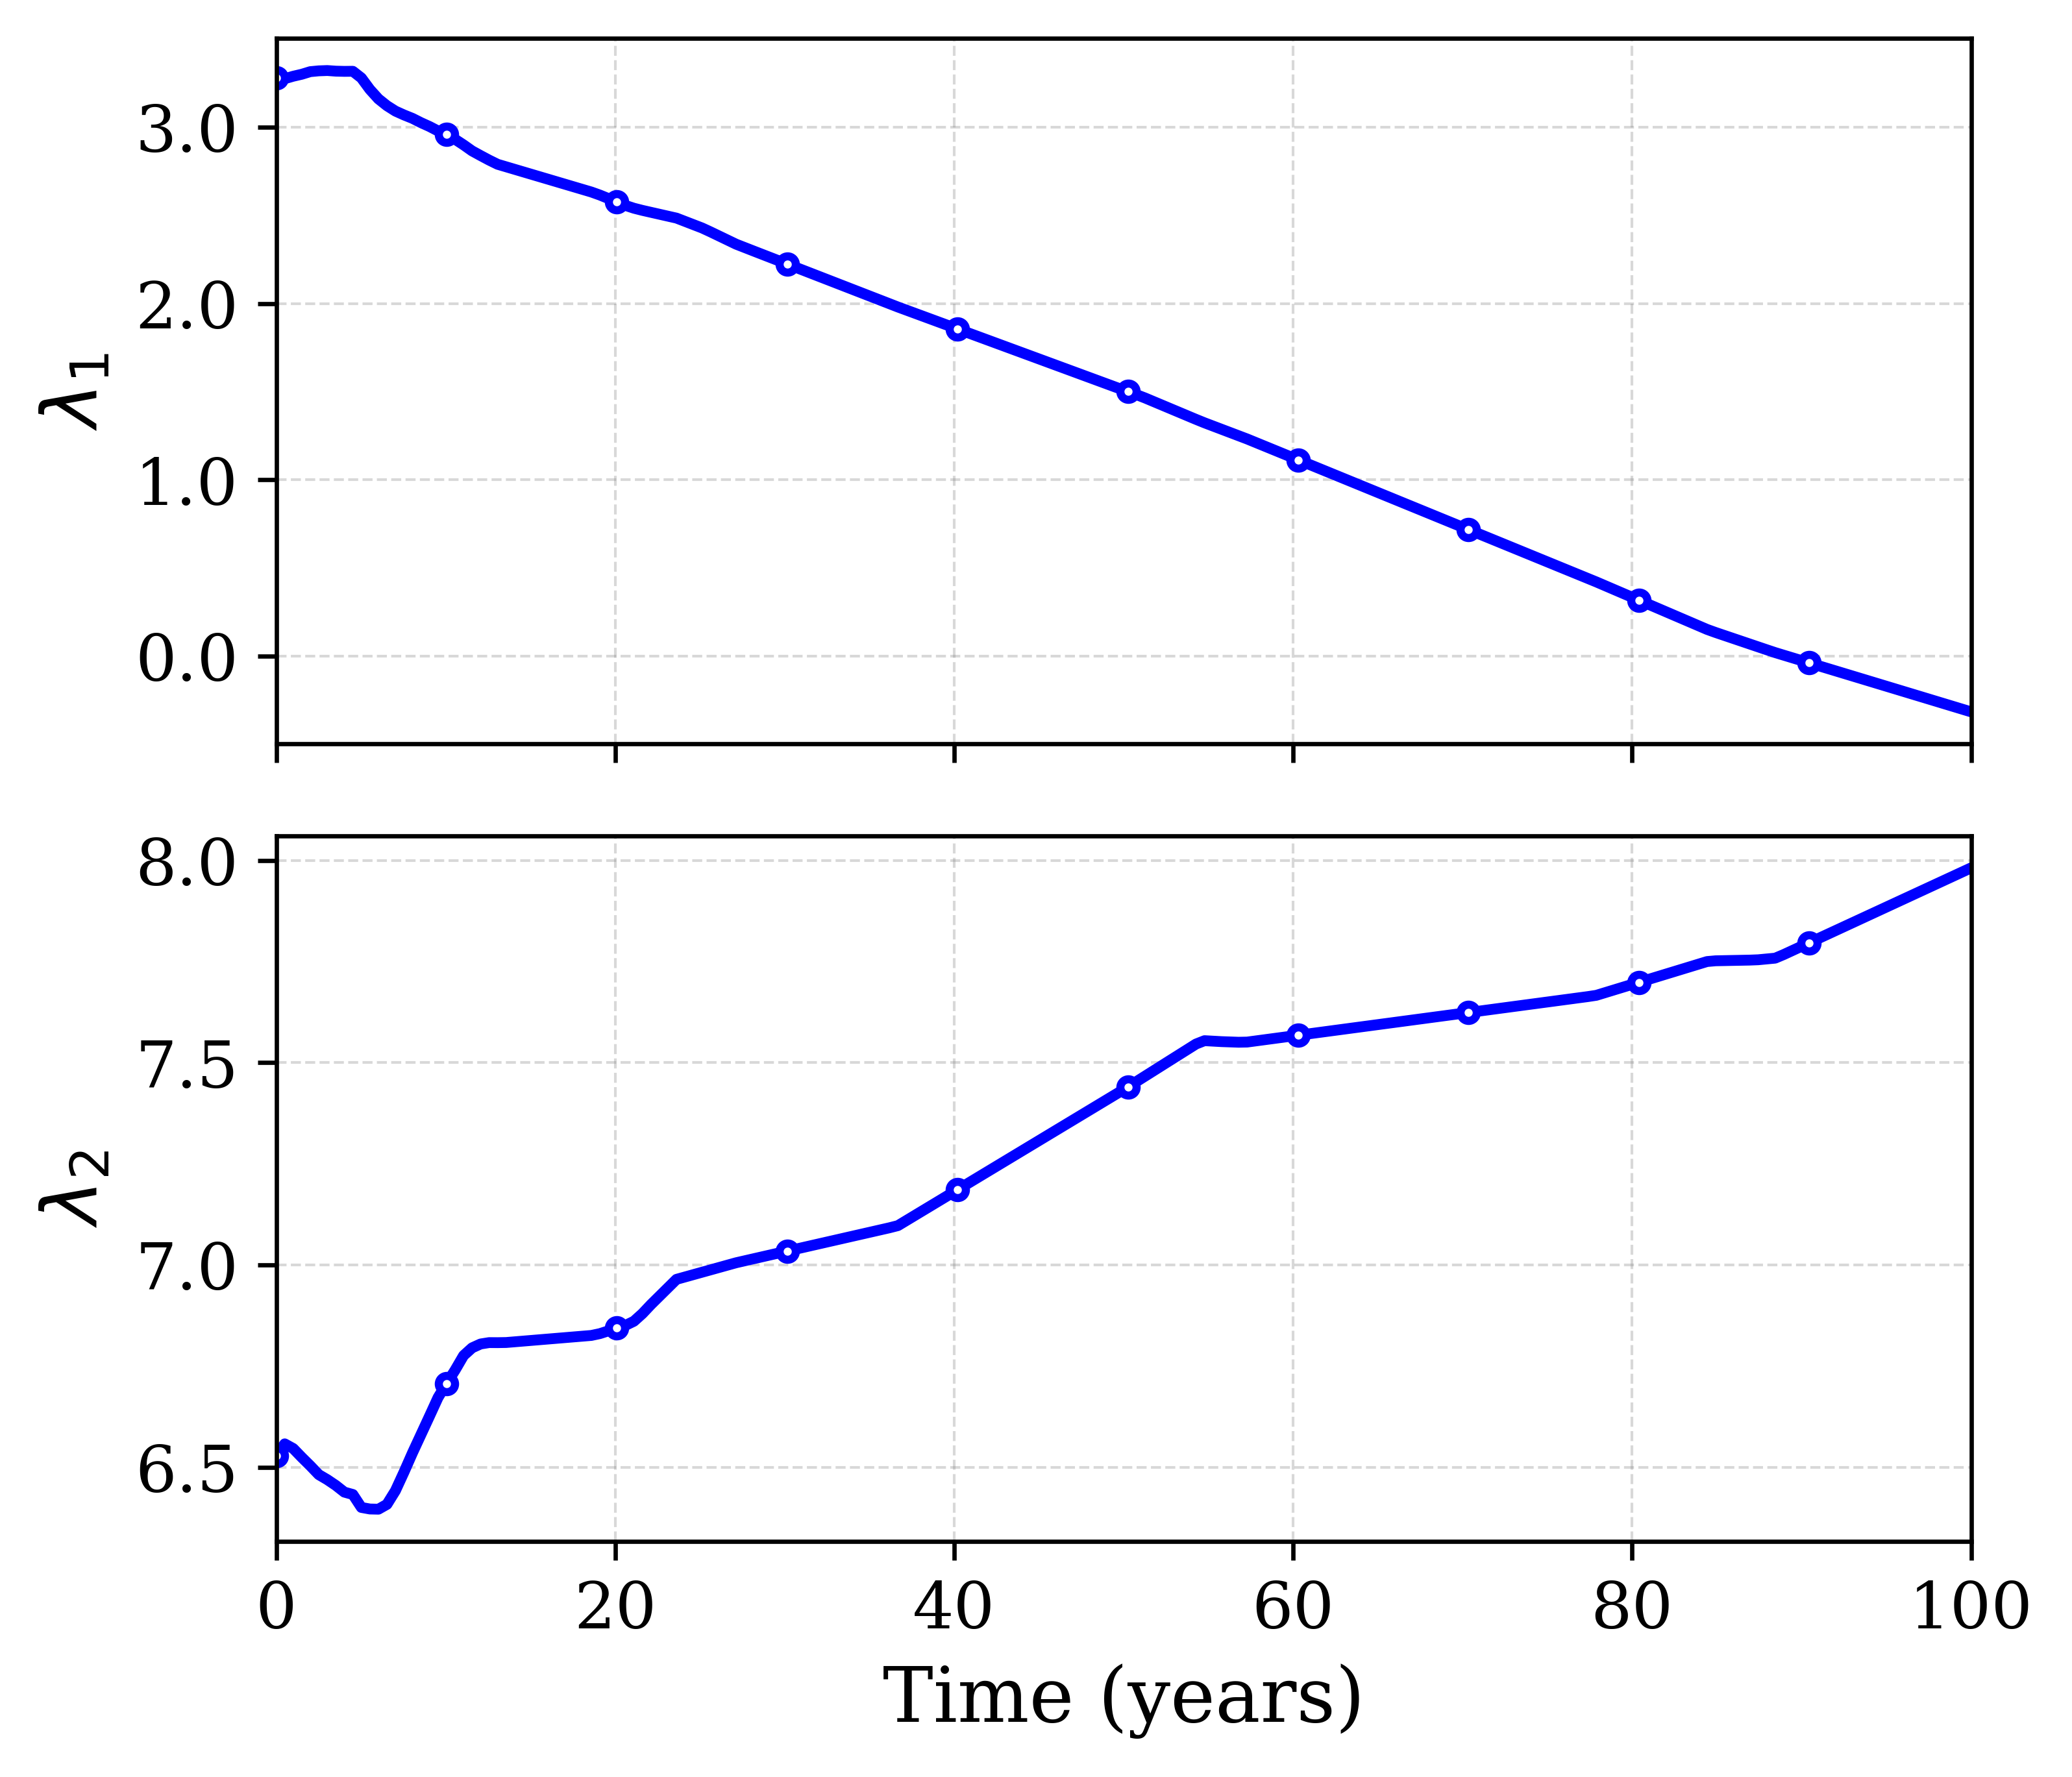
\includegraphics[width=0.75\linewidth]{z_temporal_evolution_ann_with_points_en.png}
    \vspace{0.2cm}
    \fonte{Autor (2025).}
\end{figure}

Cabe registrar que o teste mais exigente da capacidade de emulação temporal --- treinar a rede \textit{omitindo} deliberadamente um ou dois passos de tempo e comparar a densidade prevista nesses anos com a simulação direta de Monte Carlo --- ainda não foi executado. Esse experimento, previsto no cronograma revisado, é o que sustenta de forma conclusiva a alegação de emulação contínua no tempo e será conduzido tanto para o problema de referência quanto para o problema da viga.

\subsection{Vida Útil Remanescente e Custo Computacional}

Aplicando a metodologia da \autoref{sec:emulador_rul}, a Figura \ref{fig:rul_results} apresenta os produtos probabilísticos do arcabouço: a distribuição da função de estado limite no instante de inspeção de 35 anos, adotado como exemplo representativo; a densidade de probabilidade do tempo até a falha, obtida pela identificação do instante em que a trajetória de $g$ se anula, conforme a Equação \eqref{eq:ttf}; e a distribuição resultante da vida útil remanescente, Equação \eqref{eq:rul}, que consolida as incertezas propagadas e constitui o resultado central para a manutenção preditiva.

\begin{figure}[H]
    \centering
    \caption{Resultados probabilísticos do arcabouço baseado em emulador para a estimativa da VUR.}
    \label{fig:rul_results}
    \begin{subfigure}[b]{0.32\textwidth}
        \centering
        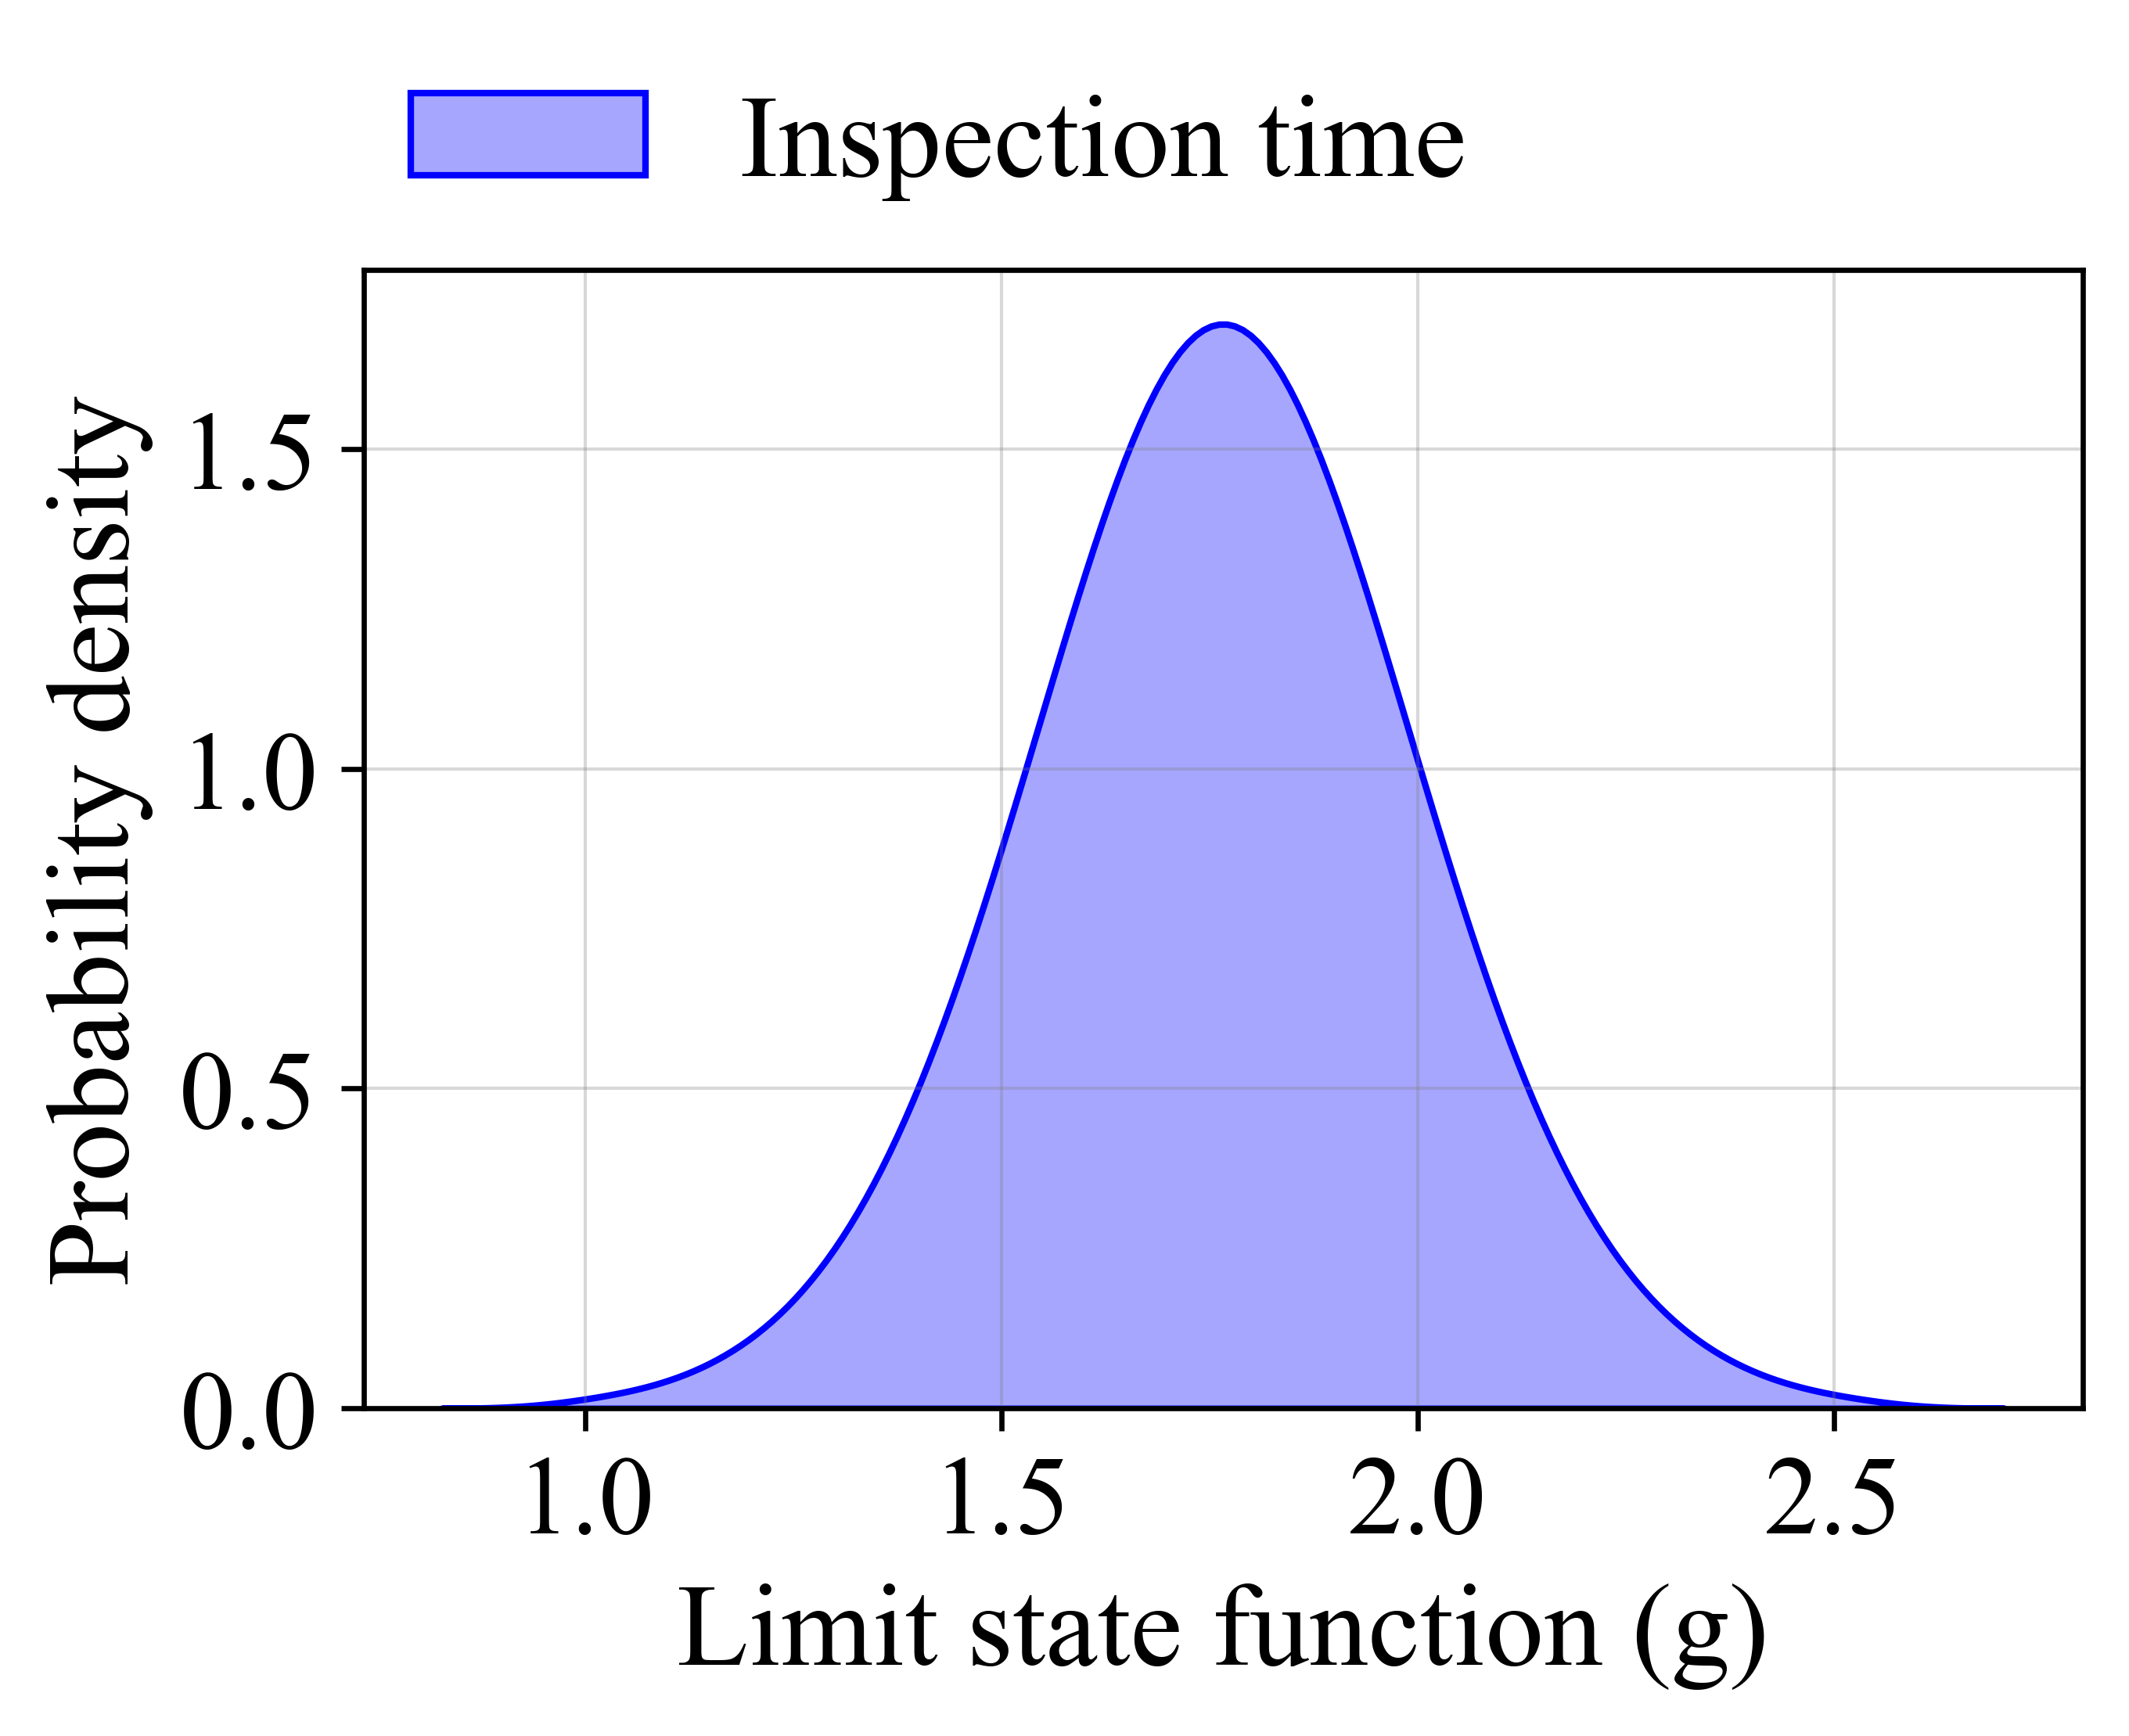
\includegraphics[height=4.0cm,keepaspectratio]{z_kde_inspection_time.png}
        \caption{$g$ no instante de inspeção.}
        \label{fig:kde_inspection_time}
    \end{subfigure}
    \hfill
    \begin{subfigure}[b]{0.32\textwidth}
        \centering
        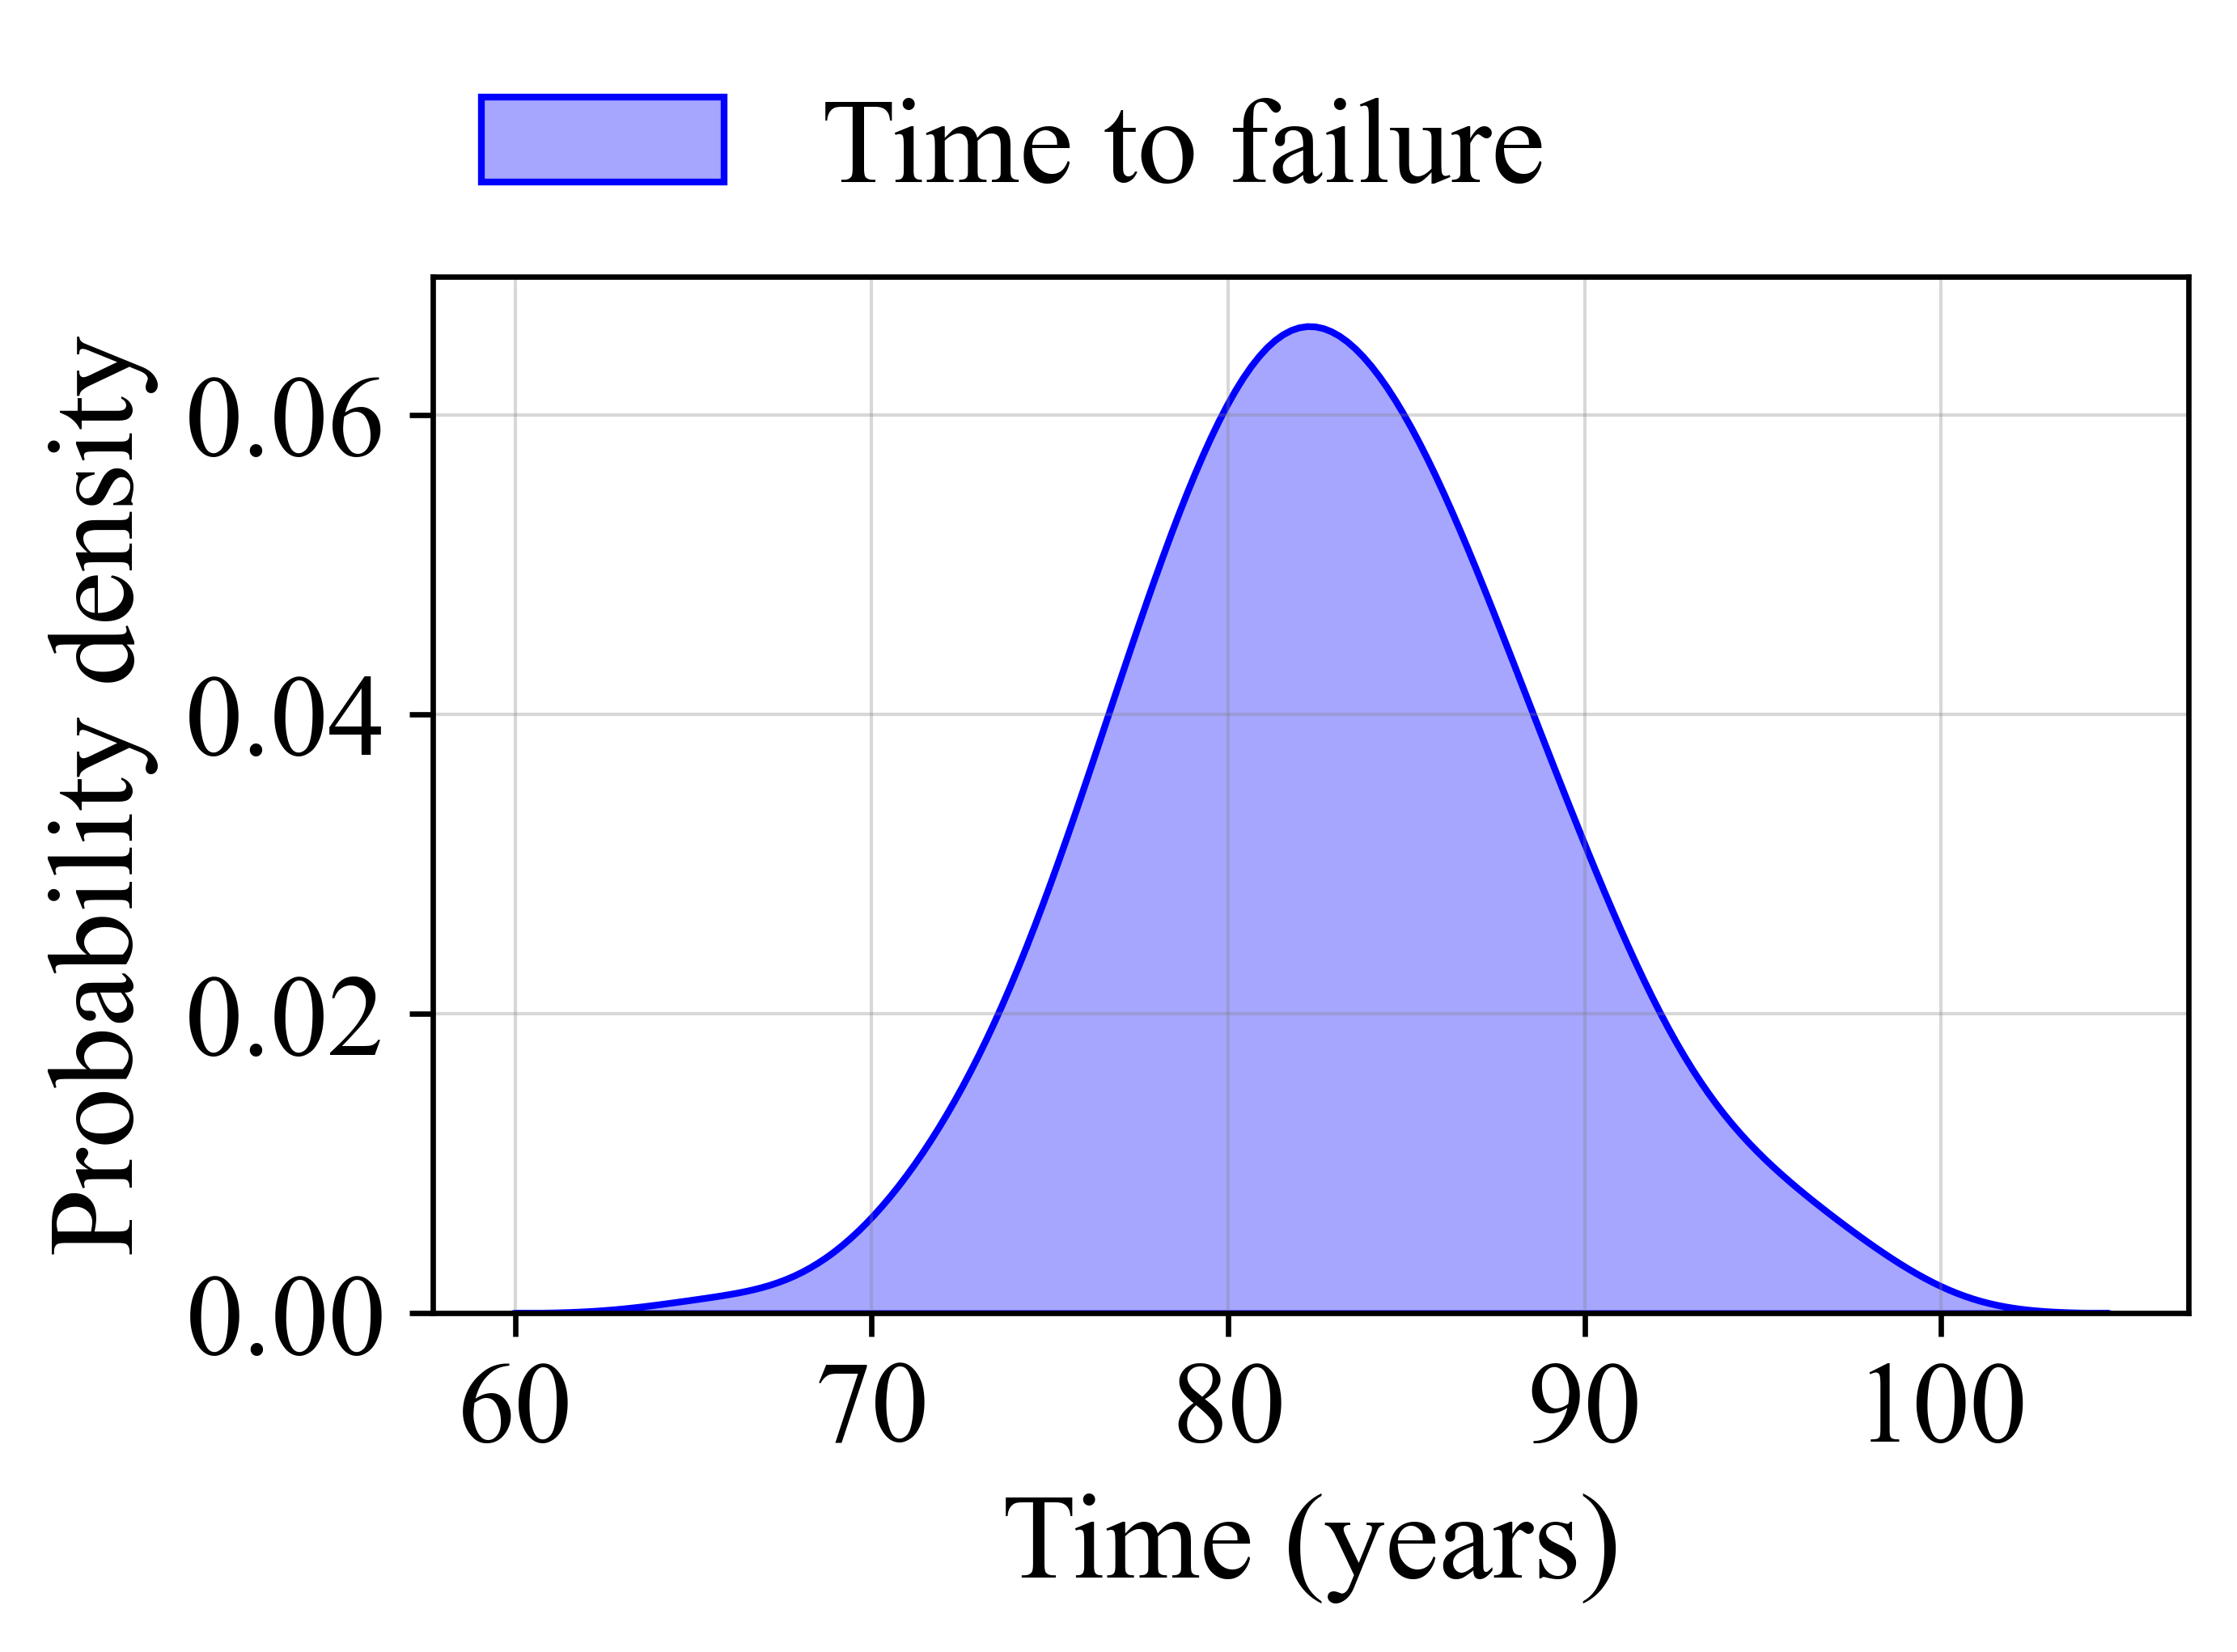
\includegraphics[height=4.0cm,keepaspectratio]{z_kde_time_to_failure.png}
        \caption{Tempo até a falha.}
        \label{fig:kde_time_to_failure}
    \end{subfigure}
    \hfill
    \begin{subfigure}[b]{0.32\textwidth}
        \centering
        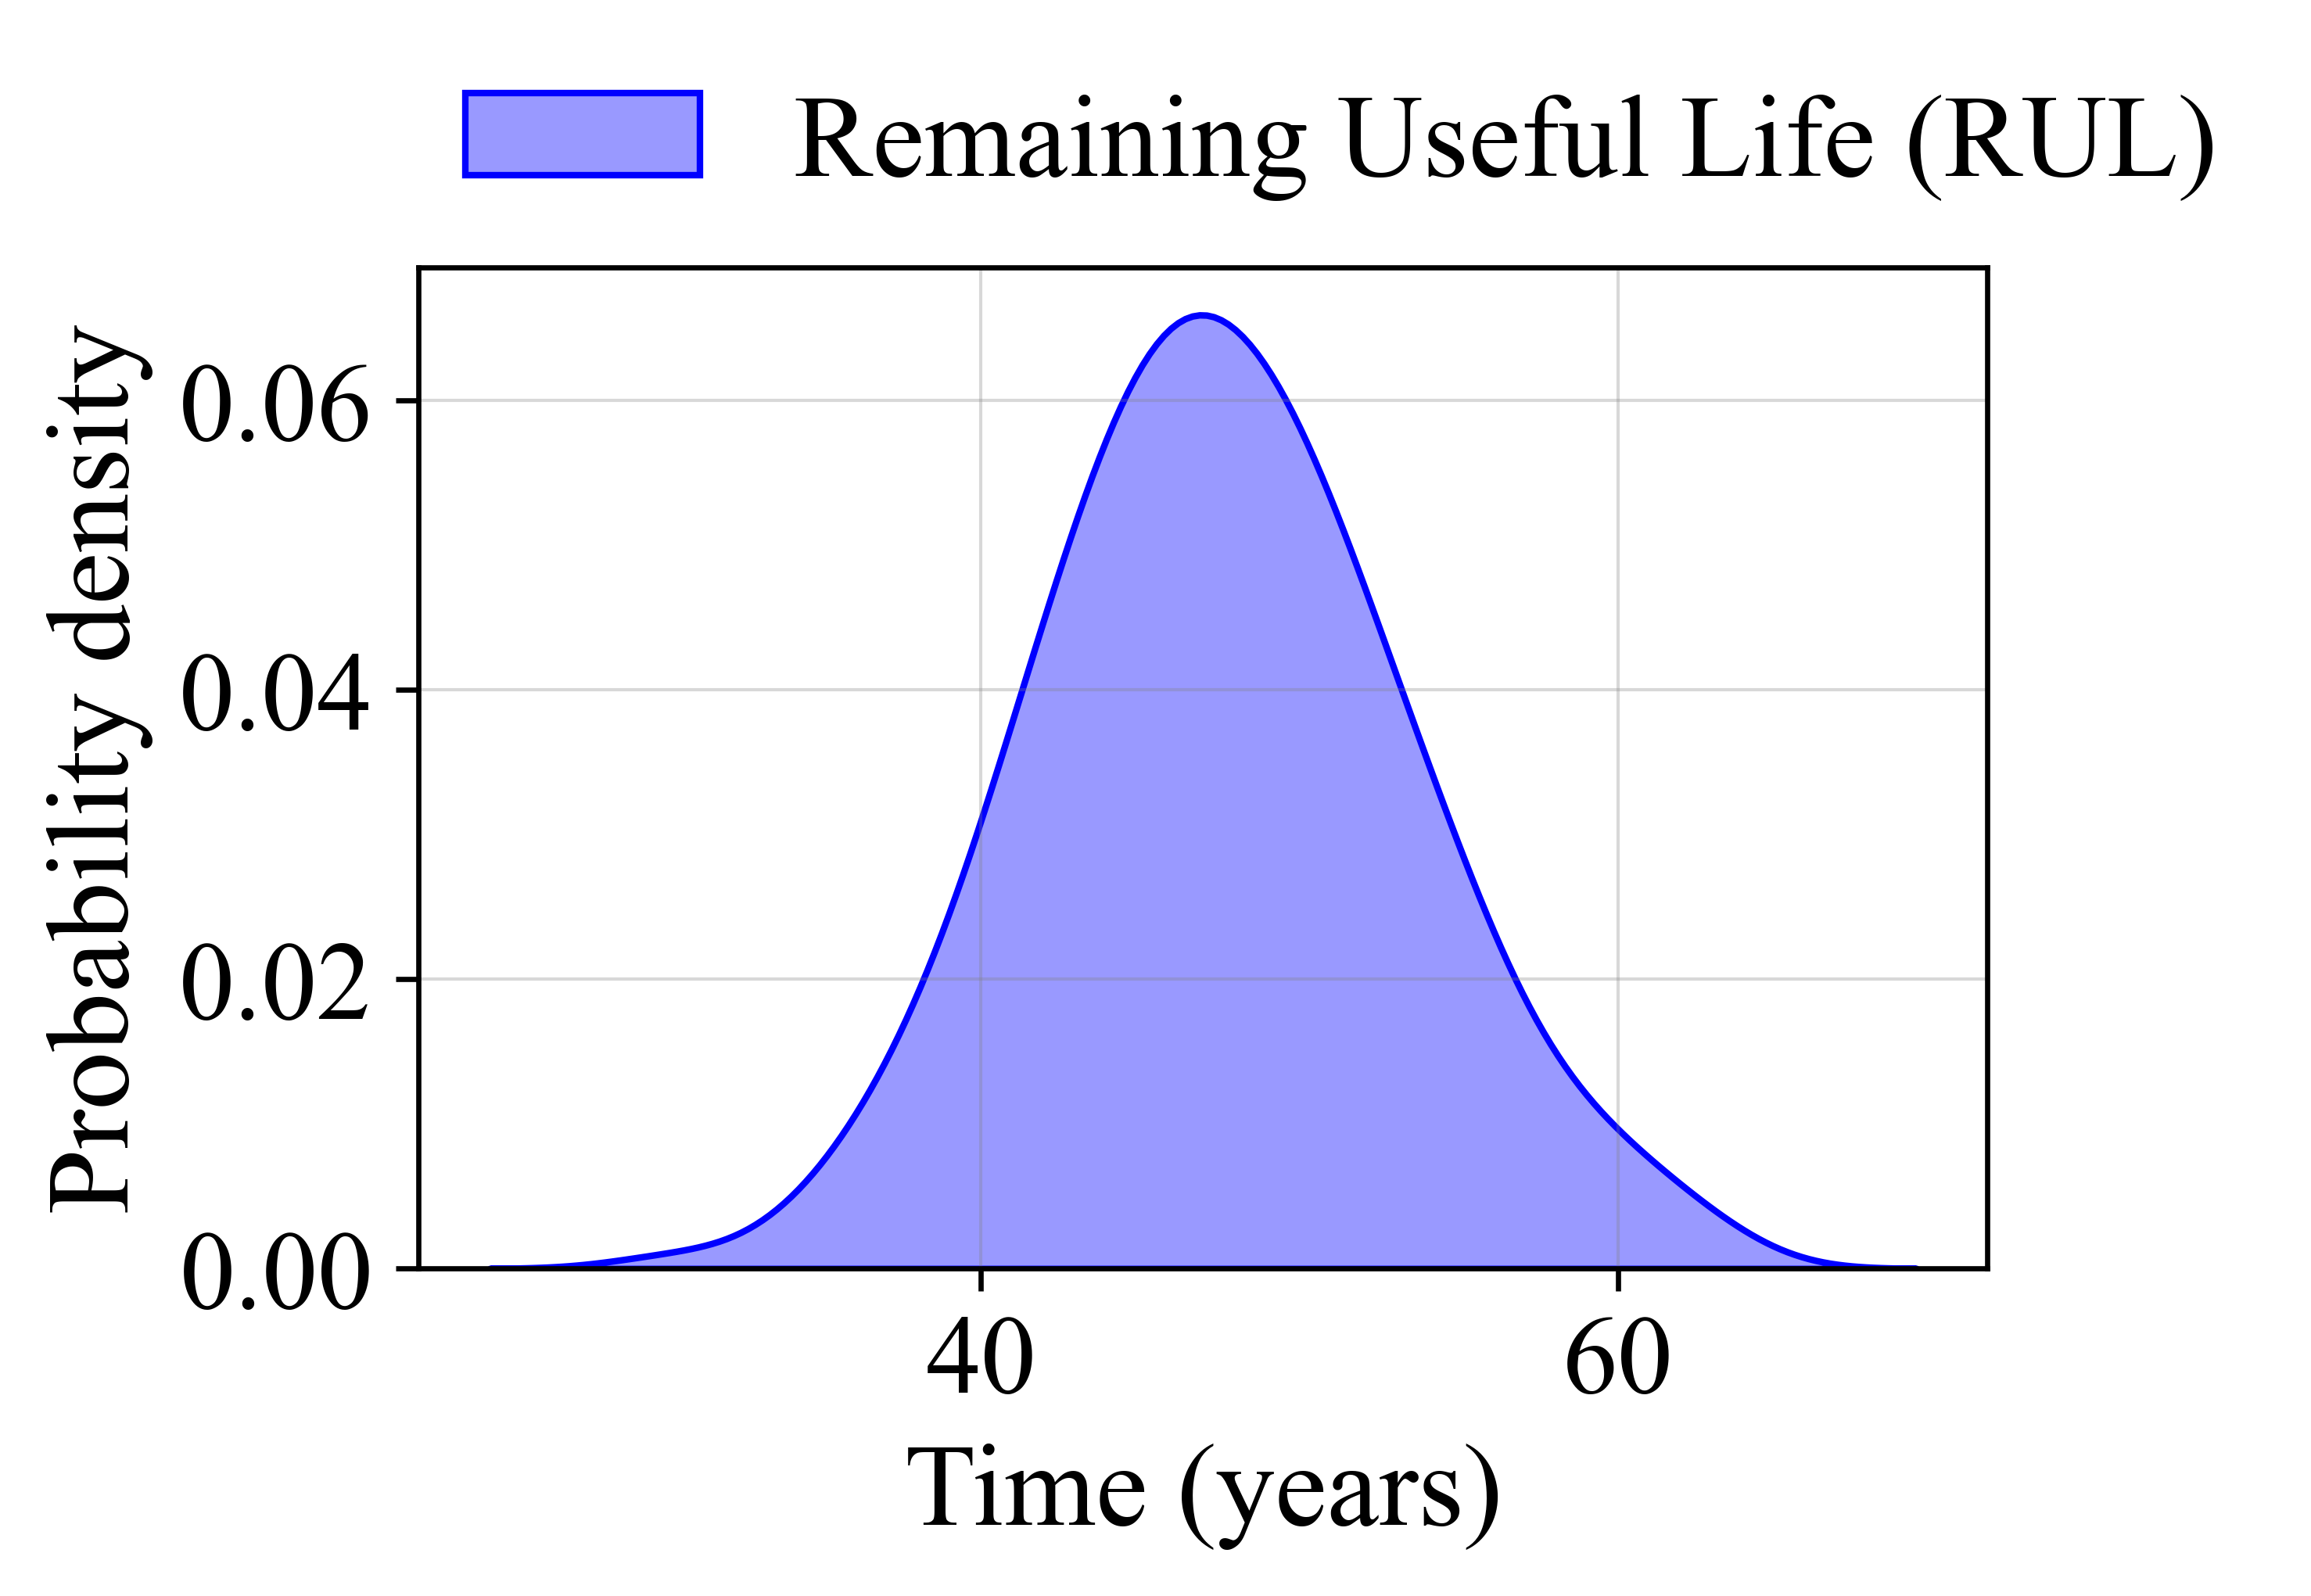
\includegraphics[height=4.0cm,keepaspectratio]{z_kde_rul.png}
        \caption{Vida útil remanescente.}
        \label{fig:kde_rul}
    \end{subfigure}
    \vspace{0.2cm}
    \fonte{Autor (2025).}
\end{figure}

Nota-se a correspondência conceitual direta entre esses três painéis e os histogramas apresentados na \autoref{sec:res_vur}: as mesmas três estatísticas de interesse --- tempo total de vida útil, valor da função de estado limite em um instante genérico e vida útil condicional --- são agora obtidas por avaliação analítica da função quantílica emulada, e não por contagem sobre amostras de Monte Carlo.

As métricas de risco derivadas da distribuição de VUR para $\alpha = 5\%$ são apresentadas na Tabela \ref{tab:var_cvar_rul}. A diferença relativamente pequena entre VaR e CVaR sugere severidade de cauda limitada, indicando que, mesmo em condições desfavoráveis, a vida remanescente prevista não exibe degradação abrupta.

\begin{table}[H]
\centering
\caption{Métricas de risco derivadas da distribuição de VUR para $\alpha = 5\%$.}
\label{tab:var_cvar_rul}
\begin{tabular}{lc}
\toprule
\textbf{Métrica} & \textbf{Valor (anos)} \\
\midrule
VaR$_{5\%}$  & 38,38 \\
CVaR$_{5\%}$ & 36,42 \\
\bottomrule
\end{tabular}
\vspace{0.2cm}
\fonte{Autor (2025).}
\end{table}

Além da acurácia das predições probabilísticas, o arcabouço oferece ganho substancial de eficiência computacional. A Tabela \ref{tab:computational_time} compara o tempo de processamento exigido pela abordagem convencional de simulação direta e pelo emulador: enquanto o procedimento convencional demandou aproximadamente 48,75~s, o emulador reduziu o custo a apenas 0,66~s, correspondendo a uma aceleração de quase duas ordens de grandeza. Esse resultado evidencia a adequação da abordagem a análises de confiabilidade e de vida útil remanescente em tempo quase real ou em larga escala, e é precisamente o que viabiliza a varredura de cenários de inspeção e manutenção pretendida na etapa final da pesquisa.

\begin{table}[H]
\centering
\caption{Comparação do tempo computacional entre a abordagem convencional e a baseada em emulador.}
\label{tab:computational_time}
\begin{tabular}{lc}
\toprule
\textbf{Método} & \textbf{Tempo computacional (s)} \\
\midrule
Abordagem convencional (Monte Carlo direto) & 48,75 \\
Abordagem com emulador                      & 0,66 \\
\bottomrule
\end{tabular}
\vspace{0.2cm}
\fonte{Autor (2025).}
\end{table}

\section{Aplicação do Emulador à Viga sob Carbonatação: Estado de Desenvolvimento} \label{sec:res_emulador_viga}

Verificado o arcabouço metodológico no problema de referência, a etapa seguinte consiste em aplicar o emulador ao problema-alvo desta dissertação: a previsão da vida útil remanescente de uma viga de concreto armado sujeita à corrosão induzida por carbonatação, com a função de estado limite da Equação \eqref{eq:estado_limite} e os modelos físicos apresentados no \autoref{cap:referencial}. Esta seção documenta o estado atual dessa aplicação e o que resta a ser executado.

\subsection{Etapas Concluídas}

Encontram-se concluídas as seguintes etapas, descritas nos capítulos anteriores:

\begin{alineas}
    \item a implementação do simulador estocástico completo, integrando o modelo de avanço da frente de carbonatação, a perda de seção e de aderência das armaduras e a verificação do estado limite último de flexão;
    \item a caracterização probabilística das variáveis básicas do problema, apresentada na Tabela \ref{tab:estatisticas_vars};
    \item a construção do banco de dados sintético por simulação de Monte Carlo com Hipercubo Latino e a extração das estatísticas de vida útil, conforme a \autoref{sec:res_vur};
    \item a implementação e a verificação da biblioteca PyGLAM para o ajuste da GLD pelo Método dos Momentos, incluindo os ensaios de aderência a distribuições-alvo conhecidas apresentados na Figura \ref{fig:pyglam_fits};
    \item a verificação do emulador PCE--GLD com camada temporal em problema de referência, conforme a \autoref{sec:res_emulador}.
\end{alineas}

\subsection{Etapas em Execução}

A transposição do emulador do problema de referência para o problema da viga apresenta duas diferenças relevantes que motivam tratamento cuidadoso. A primeira é a dimensionalidade: enquanto o problema de referência possui duas variáveis de entrada controladas, o problema da viga envolve o conjunto de variáveis geométricas, mecânicas e ambientais da Tabela \ref{tab:estatisticas_vars}, o que amplia o número de coeficientes da PCE e exige plano de experimentos mais extenso. A segunda é a natureza descontínua da função de estado limite adotada, Equação \eqref{eq:estado_limite}, cuja mudança de regime no instante de despassivação introduz um ponto de não suavidade na trajetória temporal de $g$ --- o que demanda verificação específica da capacidade da camada temporal de reproduzir essa transição.

As atividades em execução para superar esses pontos são as seguintes:

\begin{alineas}
    \item definição do plano de experimentos final, com determinação do número $M$ de pontos amostrais, do número $N$ de réplicas por ponto e dos $N_t$ passos de tempo, mediante estudo de convergência;
    \item repetição da análise exploratória de sensibilidade dos parâmetros da GLD, a fim de confirmar ou refutar, no problema da viga, a baixa variabilidade de $\lambda_3$ e $\lambda_4$ observada no problema de referência;
    \item comparação sistemática de regressores para a camada temporal --- rede neural, floresta aleatória e regressão por vetores de suporte --- com otimização de hiperparâmetros pelo mesmo procedimento adotado na \autoref{sec:res_ml};
    \item validação do emulador em instantes deliberadamente excluídos do treinamento, com comparação contra Monte Carlo direto e ênfase na cauda inferior da distribuição, região que governa a probabilidade de falha;
    \item obtenção das curvas de $p_f(t)$ e $\beta(t)$ emuladas, da distribuição do tempo até a falha e da distribuição de VUR para diferentes instantes de inspeção;
    \item análise de sensibilidade global por índices de Sobol, obtidos analiticamente dos coeficientes da PCE \cite{sudret2008}, para quantificar a contribuição de cada variável ao longo das fases de iniciação e de propagação da corrosão;
    \item avaliação de cenários de intervenção de manutenção e determinação do instante normativo de intervenção pela Equação \eqref{eq:t_man_otimo}.
\end{alineas}

A Tabela \ref{tab:estado_desenvolvimento} sintetiza o estágio de cada produto previsto para esta frente da pesquisa.

\begin{table}[H]
\centering
\footnotesize
\caption{Estágio de desenvolvimento dos produtos da frente de emulação estocástica.}
\label{tab:estado_desenvolvimento}
\begin{tabularx}{\textwidth}{X l}
\toprule
\textbf{Produto} & \textbf{Situação} \\
\midrule
Biblioteca PyGLAM (ajuste da GLD pelo Método dos Momentos)      & Concluído \\
Verificação do emulador PCE--GLD em problema de referência       & Concluído \\
Camada temporal por rede neural (problema de referência)          & Concluído \\
Distribuição de VUR e métricas de risco (problema de referência)  & Concluído \\
Teste de generalização em instantes omitidos do treinamento       & Em execução \\
Plano de experimentos do problema da viga                         & Em execução \\
Comparação de regressores para a camada temporal                  & Em execução \\
Curvas de $p_f(t)$ e $\beta(t)$ emuladas para a viga              & Previsto \\
Distribuição de VUR da viga sob carbonatação                      & Previsto \\
Análise de sensibilidade por índices de Sobol                     & Previsto \\
Cenários de intervenção de manutenção                             & Previsto \\
\bottomrule
\end{tabularx}
\vspace{0.2cm}
\fonte{Autor (2025).}
\end{table}

\section{Cronograma}

O cronograma de desenvolvimento apresentado na Tabela \ref{tab:cronograma} descreve as principais etapas previstas para a execução desta dissertação, organizadas em ordem cronológica. Cada etapa contempla um conjunto de atividades específicas, abrangendo desde a definição metodológica e o desenvolvimento dos modelos até a análise dos resultados e a redação final do trabalho. Essa estrutura visa garantir o cumprimento das metas dentro do prazo estabelecido, assegurando uma progressão coerente e integrada entre as fases teóricas, experimentais e redacionais da pesquisa.


\begin{table}[H]
\centering
\footnotesize
\caption{Cronograma de desenvolvimento da dissertação.}
\label{tab:cronograma}
\renewcommand{\arraystretch}{1.3}
\setlength{\extrarowheight}{2pt}
\begin{tabular}{>{\raggedright\arraybackslash}p{2.2cm} >{\raggedright\arraybackslash}p{3.4cm} >{\raggedright\arraybackslash}p{7.2cm} >{\raggedright\arraybackslash}p{1.8cm}}
\toprule
\textbf{Mês / Ano} & \textbf{Etapa} & \textbf{Descrição das Atividades} & \textbf{Situação} \\
\midrule

Ago/2024 – Jun/2025 &
Etapa 1 – Fundamentação e desenvolvimento metodológico &
Definição do tema e dos objetivos; levantamento bibliográfico; revisão das normas e modelos existentes; estudo de confiabilidade estrutural aplicada à corrosão; desenvolvimento dos \textit{scripts} e estruturação do banco de dados por meio de programação; verificação inicial dos parâmetros e variáveis envolvidas; desenvolvimento preliminar do modelo de confiabilidade; estruturação do texto-base da dissertação. &
Concluída \\

Jul – Ago/2025 &
Etapa 2 – Preparação e submissão de artigo a congresso &
Consolidação parcial dos resultados obtidos; elaboração de artigo técnico e submissão à conferência ARTISTE 2025; preparação e realização da apresentação. &
Concluída \\

Set – Out/2025 &
Etapa 3 – Consolidação teórica e preparação para qualificação &
Revisão e ajustes da fundamentação teórica e da metodologia; organização dos capítulos iniciais da dissertação; preparação da apresentação para qualificação. &
Concluída \\

Nov/2025 &
Etapa 4 – Qualificação &
Defesa de qualificação perante a banca; registro das observações e recomendações; planejamento dos ajustes necessários. &
Concluída \\

Dez/2025 – Mar/2026 &
Etapa 5 – Análise dos dados e formulação da função de estado limite &
Finalização do banco de dados completo; formulação e verificação da função de estado limite ($g$); checagem de consistência dos dados; execução das simulações estocásticas e tratamento estatístico dos resultados. &
Concluída \\

Abr – Ago/2026 &
Etapa 6 – Incorporação da emulação estocástica &
Estudo do arcabouço de emuladores estocásticos; implementação da biblioteca PyGLAM para ajuste da Distribuição Lambda Generalizada; acoplamento com a Expansão em Caos Polinomial; desenvolvimento da camada temporal por rede neural; verificação completa do método em problema de referência. &
Concluída \\

Set – Out/2026 &
Etapa 7 – Aplicação do emulador ao problema da viga &
Definição do plano de experimentos final; análise de sensibilidade dos parâmetros da GLD; comparação de regressores para a camada temporal; validação do emulador em instantes omitidos do treinamento. &
Em execução \\

Nov – Dez/2026 &
Etapa 8 – Confiabilidade dependente do tempo e VUR &
Obtenção das curvas de $p_f(t)$ e $\beta(t)$ emuladas; distribuição do tempo até a falha e da vida útil remanescente; métricas de risco (VaR e CVaR); análise de sensibilidade por índices de Sobol. &
Prevista \\

Jan/2027 &
Etapa 9 – Cenários de manutenção e análise crítica &
Avaliação de cenários de intervenção; determinação do instante normativo de intervenção; comparação entre a abordagem por regressão direta e a por emulação estocástica; discussão crítica dos resultados. &
Prevista \\

Fev – Mar/2027 &
Etapa 10 – Redação final e defesa &
Redação das conclusões; finalização do texto da dissertação; elaboração e submissão do artigo científico completo; defesa final. &
Prevista \\

\bottomrule
\end{tabular}
\vspace{0.2cm}
\fonte{Autor (2025).}
\end{table}

Cabe justificar a reorganização do cronograma em relação à versão apresentada na qualificação. O planejamento original previa a conclusão da pesquisa em março de 2026, contemplando a predição do tempo de vida útil por regressão supervisionada sobre o banco de dados sintético --- objetivo integralmente atingido e reportado na \autoref{sec:res_ml}. Ao longo do desenvolvimento, entretanto, evidenciou-se uma limitação conceitual dessa abordagem: a predição pontual do tempo de vida útil não fornece a distribuição de probabilidade da vida útil remanescente, que é justamente a informação necessária para a tomada de decisão de manutenção sob incerteza, conforme discutido na \autoref{TVU}.

A superação dessa limitação exigiu a incorporação do arcabouço de emuladores estocásticos, apresentado na \autoref{EMU}, cujo estudo, implementação e verificação constituíram a Etapa 6 --- não prevista no planejamento original. Essa etapa envolveu o desenvolvimento de uma biblioteca própria para o ajuste da Distribuição Lambda Generalizada e a formulação de uma extensão temporal do arcabouço PCE--GLD, que não dispõe de implementação disponível na literatura. Trata-se, portanto, de um acréscimo substantivo ao escopo, já materializado nos resultados de verificação da \autoref{sec:res_emulador}, e que fundamenta a solicitação de prorrogação do prazo para a conclusão das Etapas 7 a 10.







	% 5 - Considerações Parciais
	% ----------------------------------------------------------
\chapter{Considerações Parciais} \label{cap:consideracoes}
% ----------------------------------------------------------

Este capítulo consolida as considerações que podem ser extraídas do estágio atual da pesquisa e delimita o que permanece em aberto para a etapa final.

\section{Sobre a Abordagem por Regressão Supervisionada}

A primeira frente do trabalho apresentou uma abordagem baseada em simulação probabilística e aprendizado de máquina para a predição da vida útil de seções de vigas de concreto armado submetidas à corrosão induzida por carbonatação, utilizando um conjunto de dados sintético gerado por meio de simulações de Monte Carlo. A análise considerou variáveis geométricas, propriedades dos materiais e cargas aplicadas como aleatórias, permitindo a avaliação do desempenho estrutural ao longo do tempo por meio do índice de confiabilidade ($\beta$).

A modelagem da vida útil com base em $\beta$ mostrou-se eficaz na representação da avaliação da vida útil para uma função de estado limite baseada em flexão pura. Além disso, a incorporação de métricas de incerteza, como o intervalo de predição de 95\% (PEI95) e a largura da faixa de incerteza (WUB), reforçou a robustez dos modelos, permitindo interpretações confiáveis mesmo em cenários com alta variabilidade nas variáveis de entrada.

Diferentes algoritmos de regressão --- \textit{Elastic Net}, \textit{k-Nearest Neighbors} (KNN), \textit{Light Gradient Boosting Machine} (LGBM) e \textit{Random Forest} (RF) --- foram avaliados por meio do ajuste de hiperparâmetros. Após análise comparativa, os métodos baseados em árvores destacaram-se como os mais adequados para a tarefa, alcançando o melhor desempenho nas métricas RMSE, $R^2$, MAPE e A10, além de demonstrarem estabilidade e alta capacidade preditiva em múltiplas execuções independentes.

\section{Sobre a Abordagem por Emulação Estocástica}

A análise crítica dos resultados da primeira frente evidenciou, contudo, uma limitação conceitual relevante: o regressor supervisionado prediz um \textit{valor} de tempo de vida útil, e não a \textit{distribuição} desse tempo. As métricas de incerteza do regressor descrevem o erro de predição do próprio modelo, e não a variabilidade intrínseca do fenômeno de degradação --- grandezas de natureza distinta que não devem ser confundidas na tomada de decisão de manutenção.

A incorporação do arcabouço de emuladores estocásticos responde diretamente a essa limitação. Os resultados de verificação obtidos até o momento sustentam três considerações parciais:

\begin{alineas}
    \item \textbf{Acurácia da emulação distribucional.} No problema de referência, o emulador reproduziu a distribuição da margem de segurança com erro relativo inferior a 0,5\% até o percentil 99, com discrepâncias confinadas à cauda extrema (cerca de 1,3\% no quantil 99,9\%), conforme atestado pelo teste de Kolmogorov--Smirnov e pela comparação de quantis;
    \item \textbf{Generalização temporal.} A camada de aprendizado de máquina sobre os parâmetros da Distribuição Lambda Generalizada atuou como interpolador contínuo da distribuição entre os instantes simulados, com $R^2$ superior a 0,98 para os parâmetros sensíveis, sustentando a viabilidade da emulação dependente do tempo;
    \item \textbf{Eficiência computacional.} O emulador reduziu o custo da análise em quase duas ordens de grandeza no problema de referência (48,75~s contra 0,66~s), viabilizando a varredura de cenários de inspeção e manutenção em tempo quase real.
\end{alineas}

\section{Limitações Reconhecidas e Etapas Seguintes}

Entre as limitações já identificadas, destacam-se: a hipótese de unimodalidade da resposta, inerente à Distribuição Lambda Generalizada; a validade da interpolação temporal restrita ao horizonte de treinamento, sem garantia de extrapolação; a adoção de um único mecanismo de degradação, sem interação com cloretos ou fadiga; e a hipótese de monotonicidade da degradação assumida na relação entre a probabilidade de falha instantânea e a função de confiabilidade.

O teste conclusivo da emulação temporal --- a predição da distribuição em instantes deliberadamente omitidos do treinamento --- e a aplicação integral do arcabouço ao problema da viga sob carbonatação constituem as etapas centrais da fase final da pesquisa, conforme detalhado na \autoref{sec:res_emulador_viga} e no cronograma revisado.

Em síntese, a integração de modelos de confiabilidade, simulação estocástica e algoritmos de aprendizado de máquina mostrou-se uma ferramenta promissora para o planejamento de inspeções, manutenção preventiva e reabilitação de estruturas expostas a ambientes agressivos. A metodologia proposta reduz tempo e custo em análises complexas, contribuindo para práticas de projeto mais seguras e duráveis frente à deterioração acelerada da infraestrutura. Estudos futuros podem expandir essa abordagem incorporando outros mecanismos de degradação, como a penetração de cloretos, a atualização bayesiana do emulador com dados de inspeção em serviço e a incorporação de variabilidade espacial por campos aleatórios.

	
	% Elementos pós-textuais
	\postextual
		
	% Referências bibliográficas
	\begingroup
	    \printbibliography[title=REFERÊNCIAS]
	\endgroup
	
	
	
	% %Reconfiguração do título para apêndices e anexos
	%  \renewcommand{\ABNTEXchapterupperifneeded}[1]{#1} 
	% \makeatletter
	% \settocpreprocessor{chapter}{%
 %      \let\tempf@rtoc\f@rtoc%
 %      \def\f@rtoc{%
 %      \texorpdfstring{{\tempf@rtoc}}{\tempf@rtoc}}%
 %      }
 %    \makeatother
	
	
	% % Apêndices
 %    \begin{apendicesenv}
 %    	%\partapendices* 
 %    	\input{pos_textual/apendice_a}
 %    \end{apendicesenv}

 %    % Anexos
 %    \begin{anexosenv}
 %    	%\partanexos*
 %    	\input{pos_textual/anexo_a}
 %    \end{anexosenv}

\end{document}